%% Nemanja Milosevicr
%% phd text

%% feel free to reuse parts (or all) of the formating
%% in other words the Latex code can be used as Public Domain

%% The text itself is released under a CC-BY-SA 4.0 licence

%% Most of the code presented can be found under a GPL licence

\documentclass[b5paper]{book}

%custom packages
\usepackage[T1]{fontenc}
\usepackage[utf8]{inputenc}
\usepackage[english]{babel}

%tikz
\usepackage{pgfplots}
\pgfplotsset{width=10cm,compat=1.9}


% ovo je iz nnw template:
\RequirePackage{siunitx}
\newcommand{\doi}[1]{doi:~\href{http://dx.doi.org/#1}{\nolinkurl{#1}}}

\usepackage[autostyle=true]{csquotes}

% needs this declaration for ayodeji
\DeclareUnicodeCharacter{1ECD}{\d o}

%change the default font
\usepackage{lmodern}
\usepackage{nimbusmono}
\renewcommand{\familydefault}{\sfdefault}

\usepackage{ccicons}

\usepackage{ctable}
\usepackage{wrapfig}

\newcommand{\autor}{Nemanja Milošević}
\newcommand{\autorkratko}{N.-Milošević}
\newcommand{\naslov}{Negative Deep Learning}
\newcommand{\naslovsr}{Negativno duboko učenje}

\usepackage[style=ieee]{biblatex}

\AtEveryCite{%
  \let\parentext=\parentexttrack%
  \let\bibopenparen=\bibopenbracket%
  \let\bibcloseparen=\bibclosebracket}

\addbibresource{references.bib}

% use parens for cite

\let\oldcite\cite
\let\cite\parencite


% pdf export settings
\usepackage[%
%colorlinks,
bookmarksopen,bookmarksnumbered,citecolor=red,
%urlcolor=red,
pdffitwindow=false,unicode=true,%
pdftitle={\naslov},%
pdfauthor={\autor}%
]{hyperref}

\usepackage{graphicx}
\usepackage{fancyhdr}

\fancypagestyle{plain}{%
\fancyhead{} % get rid of headers on plain pages
\fancyfoot{}
\renewcommand{\headrulewidth}{0pt} % no lines
\renewcommand{\footrulewidth}{0pt} % 
}

% empty pages, really empty
\makeatletter
\def\cleardoublepage{\clearpage\if@twoside \ifodd\c@page\else
\hbox{}
%\vspace*{\fill}
%\begin{center}
%This page intentionally contains only this sentence.
%\end{center}
%\vspace{\fill}
\thispagestyle{empty}
\newpage
\if@twocolumn\hbox{}\newpage\fi\fi\fi}
\makeatother

% put figures in the figures folder
\graphicspath{{./figures/}}

\usepackage[figure,table,page]{totalcount}

\newcounter{citenum}
\AtEveryBibitem{\stepcounter{citenum}}

\usepackage{amsthm}
\usepackage{amsmath}
\usepackage{latexsym}

\usepackage{listings}

% if we want to make an index at the end we need this
% this document didn't have an index in the end
%\usepackage{makeidx}

%\makeindex

\lstset{
        basicstyle=\small\ttfamily,
        showstringspaces=false,
        breaklines=true
}

\lstloadlanguages{Python}

\lstnewenvironment{codeblock}
{\lstset{basicstyle=\footnotesize\ttfamily,
        columns=fixed}}
{}

%options to the lst can be given through this
\lstnewenvironment{codeblock1}[1]
{\lstset{basicstyle=\footnotesize\ttfamily,#1,
        columns=fixed}}
{}

\lstnewenvironment{codeblockw}
{\lstset{basicstyle=\footnotesize\ttfamily,
    language=wsl,
        columns=fixed}}
{}
\lstnewenvironment{codeblocka}
{\lstset{basicstyle=\footnotesize\ttfamily,
    language=[x86masm]Assembler,
        columns=fixed}}
{}
\lstdefinestyle{asmblock}{
  language=[x86masm]Assembler,
  basicstyle=\footnotesize\ttfamily
}
\lstdefinestyle{codeblock}{
        basicstyle=\footnotesize\ttfamily,
        columns=fixed,
        language=wsl
}

\lstdefinestyle{codeblockb}{
        basicstyle=\normalsize\ttfamily,
        columns=fixed,
        language=wsl
}


%% `skica' is Serbian for `sketch', these blocks were used in the development
%% of the document for various reminders

% skica can take a normal paragraph and present it more or less as such
\newcommand{\skica}[1]{
    \noindent \framebox{\parbox[c]{0.9\textwidth}{  {\small** {#1}  }}
    \newline }
}

% skicas is a small sketch, intended mostly for inline use
\newcommand{\skicas}[1]{
    \framebox{* \small \textit{#1} *}
}

% b is for bold sketches, things that are high priority
\newcommand{\skicab}[1]{
  \noindent \framebox{\parbox[c]{0.9\textwidth}{ {\small***
        \textbf{#1} }} \newline } }

% special words inline such as class and method names
%\newcommand{\kod}[1]{{\small\texttt{#1}}}
\newcommand{\kod}[1]{\lstinline[]`#1`}
\newcommand{\code}[1]{\lstinline[]`#1`}
\newcommand{\codea}[1]{\lstinline[style=asmblock]`#1`}
\newcommand{\codew}[1]{\lstinline[style=codeblock]`#1`}

%% these commands were used to get a clean version of the text
%% without the sketches

%\renewcommand{\skica}[1]{}
%\renewcommand{\skicas}[1]{}


% experimental, for one line of par being split over a page
\widowpenalty=10000
\clubpenalty=10000

% ----------------===========--------------------------------------
%                 start paper


\author{\autor}
\title{\naslov}
\date{Novi Sad, 2021}
\begin{document}
\frontmatter

\newcommand{\makemytitle}{
  \begin{center}

	
\includegraphics[width=1.8cm]{pmf-logo}\hspace{\stretch{1}}
	\parbox[b]{45ex}{\centering
          University of Novi Sad\\
Faculty of Sciences\\
Department of Mathematics and Informatics\\ }\hspace{\stretch{1}}
	
\includegraphics[width=1.8cm]{uns-logo}

	\vspace{15ex}

	\parbox[b]{\textwidth}{{\Large {\bf \hspace{0.5cm}Nemanja Milošević}}}
	\vspace{4ex}

	{\huge
            \setlength{\baselineskip}{1.5\baselineskip}\textbf{\naslov}\par}

	\vspace{4ex}
	-- Doctoral dissertation  --

        \vspace{5ex}

	{\huge
            \setlength{\baselineskip}{1.5\baselineskip}\textbf{\naslovsr}\par}

	\vspace{4ex}
	-- Doktorska disertacija  --

	\vfill

	Novi Sad, 2021
	\end{center}
	\thispagestyle{empty}
	\newpage
}

\makemytitle

~

\vfill

\thispagestyle{empty}
\noindent CC BY-SA \ccbysa\\
\textcopyright \ 2021 Nemanja Milošević\\
This work is licensed under a
Creative Commons Attribution Share Alike 4.0 International Licence
\url{https://creativecommons.org/licenses/by-sa/4.0/}

\chapter{Preface}

Artificial Intelligence is one the fastest growing fields in Computer Science. Recent developments in hardware and software mean that now, more than ever, AI can be used in a large number of fields and problems. Even though the fields such as Machine Learning and Deep Learning are already at a stage where they can be, and are used every day, there is still a long way before we can use AI which performs similarly to humans with confidence. 

AI is now present in our day-to-day life. Even devices we wear, such as mobile phones, or smart wear, are now capable of recognizing patterns in our behaviour and reacting to a degree we allow them. A smart watch knows what type of exercise we are performing just as our mobile phones know whose picture we are taking. 

In an AI-driven world, we want algorithms and models which we can rely on. In critical systems specifically, but also in every day life. The problem is that many of the high performing models, especially deep neural networks, are difficult to understand and interpret. We have to develop methods and ways to validate models behaviour, especially in difficult situations. A self-driving car must know how to react if its cameras views are obscured by snow or ice. That is why, now and in the future a great deal of attention must be given to improve robustness and interpretability of these models we intend to rely on. New models, architectures and specificities must be discovered and applied to the problems we are having. In this thesis we describe several such models, a variety of negative deep learning models, which are more robust and perform better in difficult scenarios, when compared to existing approaches. We show empirical results which prove that negative deep learning models when trained properly can bring robustness and performance in agent environments, partial input classification, occlusions, adversarial attacks and other challenging tasks.

This PhD thesis is split into five main parts.

In Part 1 we provide a short introduction and overview of the field, introducing some aspects we will need later to define our negative deep learning models.

In Part 2 we discuss about possible implementations of negative learning models and provide some examples and where they can be applied.

In Part 3 we introduce the first negative learning model which can classify instances based on their missing features. We provide detailed explanation on how the model was implemented and tested. We also present all the different experiments that were performed, their results and the discussion of the outcomes.

In Part 4 we discuss an interesting characteristic of the previous model we discovered and how it led us to develop the Synergy model -- another negative deep learning model. We validate our assumptions again with various experiments and results.

In Part 5 we discuss what we call "true" negative deep learning models, models which only learn from negative data. We discuss existing approaches and showcase one of our own: a negative Siamese Triplet Loss neural network. Finally, we discuss how negative deep learning can be used in agent environments and provide one example environment where the agent's behaviour can be controlled only with negative rewards (punishments).

\section*{Acknowledgements}

Firstly, I thank my mentor, Dr.~Miloš Racković for the time we spent working on this thesis, the initial idea of negative learning and the time spent working on the papers which contributed to this thesis, over the years. Among other things, he taught me how to express myself in a clear, concise way, which greatly contributed to my academic and teaching activities. I thank him for many long discussions and e-mail threads we shared whenever I did not know how to proceed in my research. I would also like to thank the members of the committee, Dr.~Jelena Slivka, Dr.~Miloš Radovanović, Dr.~Srđan Škrbić and Dr.~Vladimir Lončar, for their time spent on reading and commenting this thesis.

I thank the Faculty of Sciences, University of Novi Sad for some of
the facilities that were used during the development of this thesis, especially for the hardware (axiom cluster) that was needed for all the experiments performed during production of this PhD thesis.

A special thanks goes to professors Dr.~Dušan Jakovetić and Dr.~Srđan Škrbić for our successful cooperation on many international projects related to Machine Learning and Artificial Intelligence which pushed me forwards in my knowledge and capabilities.

The largest thanks goes to my family and friends for their continuous support during my career. 

I thank my father Branislav for transferring his love for programming to me, my mother Jasmina for teaching me to value important things in life and never give up no matter what, my other mother Tamara for keeping our family together and my brother Aljoša and sisters Tamara and Teodora for the endless time we spent playing video games together.

I thank my friends Dragana, Doni, Milan and Tanja for constantly asking me "how is the thesis going and when will you finish" and for all the PhD and research related memes they have sent me over the years. 

Finally I thank my world Nataša Sukur for everything she has done for me, pushing me to move forwards in the hardest of times. Without her I would not be who I am and without her support this thesis would never exist.

\chapter{Rezime}

U današnje vreme upotreba dubokog učenja radi prepoznavanja određenih paterna u podacima postala je nezamenljiv alat u mnogim sistemima. U kritičnim sistemima pogotovo, duboke neuronske mreže se često koriste čak i u scenarijima koji direktno utiču na naše živote. Upravo to je razlog što se u poslednje vreme u istraživanju sve više stavlja akcenat na duboko razumevanje ovih modela i na modele koji su dokazano pouzdani, robusni i sigurni za upotrebu.

U ovoj doktorskoj disertaciji istražujemo negativne modele dubokog mašinskog učenja kao novi pristup razvoju modela sa visokim performansama i još važnije sa povećanom robustnošću i pouzdanošću u poređenju sa modelima današnjice. Takođe se bavimo nadogradnjama postojećih modela sa našim negativnim pristupom i pokazujemo kako se postojeći modeli mogu unaprediti bez velikih promena u arhitekturi.

Kod modela za klasifikaciju slika (danas najrasprostranjenija primena dubokih konvolutivnih neuronskih mreža) pokazaćemo kako se ovi modeli mogu nadograditi i izmeniti kako bi u obzir uzimali i negativne osobine -- one osobine koje znamo da postoje a nisu trenutno prisutne u ulaznim podacima.

Za sve modele predstavljene u ovoj disertaciji biće prikazana duboka analiza procesa kao što su negacije osobina, negativne aktivacione funkcije, zamrzavanje slojeva neuronskih mreža, transfer znanja iz jedne mreže u drugu, fine-tuning pristup treniranju, inverzije konvolutivnih filtera i drugo.

Dodatno znanje, u obliku negativnog znanja, može biti veoma bitan faktor u učenju i kreaciji modela koji imaju povećanu preciznost, pouzdanost i robustnost, pogotovo u teškim situacijama. Definišemo teške situacije kao one situacije u kojima je model suočen sa podacima koji su izmenjeni ili teži za razumevanje na neki način, bilo na prirodan način ili veštački način. Na primer, modeli predstavljeni u ovom radu su testirani u slučajevima parcijalnih ulaza i okluzija gde su delovi ulaznih podataka odstranjeni ili zaklonjeni na neki način. Negativni modeli u ovakvim situacijama imaju znatno više performanse u poređenju sa običnim, tradicionalnim modelima iste arhitekture. Za veštački generisane situacije, govorićemo o adversarijalnim mrežama, podacima i napadima i kakve su performanse naših negativnih modela kada se suoče sa takvim podacima. Testirani su black-box i white-box adversarijalni napadi i odabrani su oni napadi koji danas predstavljaju najnaprednije moguće metode za namerna kvarenja modela dubokog učenja.

U ovoj disertaciji takođe uvodimo pojam mreže sinergije, koja predstavlja spoj normalne i negativne mreže i kao takva se može koristiti i primeniti na bilo koji postojeći model. U sinergiji deo mreže ili cela mreža se dodaje na postojeći model u kombinaciji sa određenim modifikacijama kako bi se uključilo negativno duboko učenje. Pokazaćemo da ovakvi modeli imaju još više performanse u poređenju sa negativnim modelima i eksperimentisaćemo sa raznim načinima spajanja mreža. Model sinergije će biti testiran na CIFAR10 skupu podataka dok su negativni modeli razvijani i testirani na MNIST i EMNIST skupovima podataka.

Na kraju, govorićemo o modelima koji koriste "pravo" negativno učenje, a to su oni modeli koji koriste samo negativno znanje za učenje. Biće dat prikaz postojećih sličnih modela kao što su Negative Sampling modeli, Noisy Label Classification modeli i modeli koji koriste Noise Contrastive Estimation. Naš fokus je na dva modela za koje ćemo predložiti i implementirati nadogradnje a to su: negativna Deep Q-Learning agentska neuronska mreža i negativna sijamska Triplet Loss mreža. Oba ova modela mogu biti korišćena uz pomoć samo negativnih podataka, u nekim slučajevima za potpuno treniranje a u nekim slučajevima kao vid regularizacije.

\chapter{Abstract}

In recent times the use of Deep Learning as a tool for pattern recognition and more has become essential for many tasks. In critical systems specifically these models are often used in human life affecting environments and that is the reason for new and recent research regarding these models and and their robustness and reliability. 

In this thesis we explore negative deep learning as a new approach to developing models which have higher performance and more importantly increased robustness compared to normal models used today. Moreover we show how many existing models can be upgraded to employ some kind of negative deep learning without large architectural changes.

We will discuss how image classification neural networks (most popular use case of the convolutional neural network family) can be modified to take into consideration missing (negative) features from input samples when making their decisions. 

We provide deep explanation of the feature negating process, experimenting with different activation functions, neural network layer freezing, Transfer Learning and Fine Tuning approaches, convolutional kernel inversions and more.

We show that by employing this additional knowledge we create models with increased robustness, especially in difficult scenarios. We define difficult scenarios as those which are naturally or artificially difficult for modern neural networks. For example, we benchmark our models in the cases of partial input examples and occlusion against normal models of same architecture to show our modifications bring performance and robustness is this type of classification tasks. For artificial scenarios, we show that our models are less susceptible to adversarial attacks, both white-box and black-box. We test with state-of-the-art adversarial algorithms and see various level of improvements for different attacks and datasets (MNIST, EMNIST variants).

In this thesis we also introduce the notion of a Synergy model, a model which is a pure upgrade of any neural network model where additional model, or part of it, is appended with the negativity embedded into the underlying signal processing. We show that the Synergy models can generally outperform our negative models without any performance penalty when comparing to normal models. We also experiment with different state-of-the-art Ensemble network joining methods and show how they differ in implementation effort and performance. The synergy models is tested against more complex CIFAR10 dataset and its adversarial modifications, both human and artificial.

Lastly we mention true negative deep learning models, which are those which use only negative knowledge for learning. An overview of existing models is provided including Negative Sampling, Noisy Label Classification and Noise Contrastive Estimation. We focus on two models for which we provide upgrades and implementations: a negative Deep Q-Learning agent in a Deep Reinforcement Learning Task and a negative-only Siamese Triplet Loss network. Both these models, we show, can be used in a negative-only scenarios, some for regularization purposes, some for complete training.

\tableofcontents

\mainmatter

\part{Introduction}
\chapter{Artificial Intelligence: A brief overview}

In the first part of this dissertation a short history of the field is presented with focus on some models and approaches used later to define and describe negative deep learning models. 

Artificial intelligence is a universal field. Whether it is writing poetry, playing chess, proving theorems, self-driving cars or any other intellectual task, throughout history scientists have tried different artificial intelligence (AI) methods to bring the machines closer to us humans. Even though we think AI is the "new and hot" field in Computer Science, modern AI roots can be traced all the way to World War II. The name was coined after (in 1956) but the science was there long before that. From Alan Turing to Yann LeCun and others, generations have been working hard to bring the dream closer to reality -- a dream where machines can think, and reason. From the iconic Turing test to the deep neural networks, we have come long way but we still have loads to discover.

\section{History of Artificial Intelligence}

Many have tried to precisely define what AI means. Today, we know that a single, all encompassing definition is very difficult to formulate. AI is concerned with reasoning, behaviour, thought process, rational thinking and other well-defined terms. Therefore we define AI as a sum of everything that makes machines perform closely to human level. In other words machines need to learn to do the "right thing", given the knowledge we possess.

In the early days of AI, researchers sought ways to solve difficult problems for humans. These problems proved to be easy for machines to comprehend through a series of formal, mathematical rules. The real challenge today is solving the tasks that easy for humans but hard to describe formally -- problems that feel automatic, intuitive like recognizing spoken words or faces in images. \cite{goodfellow2016deep}

To try and provide the scientific world with an operational definition of intelligence, Alan Turing (1950) devised the famous Turing Test. A machine (in other words software) passes the test if a human asking series of questions cannon tell whether the responses are coming from a person or a computer. To develop software able to do this is not an easy task. The system would have to have many capabilities including: natural language processing (so it can communicate), knowledge representation (so it can store what it knows), automated reasoning (to draw conclusions from the knowledge) and machine learning (to adapt to new environments and detect and understand patterns in knowledge). In addition to these capabilities if we were not to avoid human-machine physical contact, the machine would also have to be able to see (computer vision) and interact with the real physical world (robotics). The six capabilities remain relevant today, 70 years after the Turing Test was formulated.

Today, researchers are not pursuing the solution to the Turing Test actively as before. The reason in in believing that it is more important to study the underlying principles of intelligence, than to duplicate it. 

With that in mind, comes the state-of-art-approach as of today -- Deep Learning.

Our "seat of consciousness", the brain, is the main object of study in neuroscience. Even though even today, the exact way in which the brain functions remains one of the great (if not the greatest) mysteries of science, the simple fact that it does enables the drive of researchers to push further and further in the quest of fully understanding the how and the why. In the 18th century, humanity was certain that the brain is the center of reason in humans, and in the 19th century we were made aware the brain contains many neurological cells called neurons. (Golgi, Broca) In the early 20th century, Nicolas Rashevsky was the first to apply mathematical models in studying the nervous system. 

Neurons or nerve cells are built from two major parts: cell body (soma) which contains a cell nucleus and a number of fibers called dendrites on of which is longer than the others (axon). Axon length is particularly interesting, some can be up to a meter long. A typical biological neuron makes connections with 10 to 100000 other neurons at junctions which are called synapses. Signals are propagated though neurons by the means of a complicated electrochemical reaction. The signals are used to control brain activity but can also enable long-term changes in connections between neurons. We believe that these mechanisms enable our brains to learn. It is amazing to think that a structure of simple cells can lead to thoughts or that in other words: brains cause minds (John Searle, 1992). \cite{searle1992rediscovery}

\section{Reappearance of Neural Networks with modern hardware development}

With modern GPU (graphical processor unit) development, especially the developments related to the NVIDIA CUDA framework, deep neural network models were suddenly possible and obtainable.

The human brain consists of around 100000000000 neurons (\(10^{11} \)). A modern computer can have even more transistors, thus we are approaching singularity -- a point in time where computers reach superhuman levels of performance. The raw comparison is not especially informative (or right) since that even if one made a computer with unlimited resources and capabilities, we still would not know how to achieve brain's level of intelligence.

In the mid 1980s at least four different research groups revisited backpropagation learning algorithm developed 20 years earlier by Bryson and Ho. \cite{lecun1988theoretical} The so called connectionist model was seen by some as a direct competitor to previously developed symbolic models and also to the logicist approach. The current view is that all these approaches are complementary, not excluding.

\section{Modern Machine Learning}

As algorithms developed and we learned more and more about intelligence, one thing was very clear: AI systems must have the ability to acquire their own knowledge. This is done by extracting knowledge (patterns) from raw data. The performance of the system still relies heavily on the operator in crucial way and that is the was the data is represented. This is why almost all algorithms require specific data presented in a specific way in order to be useful. Each piece (called feature) of information can be very important. Machine learning algorithm outcome is influenced by the feature values, in other words the algorithm learns to correlate these feature values and the outcome values.

In many tasks it is very difficult to define data structures in a way that it is easy to extract meaningful feature values. This is why researchers rely on fields like representation learning where the algorithm is forced to not only provide some reasoning or outcome of the feature value inputs but also a different, more efficient representation of the input features. These representations can be very complex and difficult to interpret and that is why today we rely on stacking many simplified versions of them. If we were to draw the structure of these algorithms we would need a lot of space, because we can make them very deep. So deep in fact that they are called: Deep Learning algorithms.

\section{Deep Learning and its common uses}

Deep Learning uses stacked feature representations to define complex relationships between input patterns and output data. With Deep Learning, we can build complex concepts out of simpler concepts, and that is a very powerful paradigm. 

The simplest example of this concept is a multilayer perceptron (MLP). \cite{russell2002artificial} This structure is a simple mathematical function mapping a set of input values to a set of output values. However, the beauty of it is in that the complex function (MLP) is built from other simpler functions of which they are many. Every calculation of formulas applied to any data point inside a MLP can be thought as a new representation of the input data. MLP's and other similar models are often called Universal Function Approximators. 

The main idea of Deep Learning (DL) \cite{lecun2015deep} and its stacked representations of the input data provides one perspective in which we judge different DL algorithms. Another perspective comes also from depth but in slightly altered way. By using many layered representations of data we allow the machine to process data in a series of steps which is very important for some tasks and makes the algorithms learn better as they focus on smaller steps at a time. The deeper the network, the larger is the number of steps taken towards the solution. Sequential reasoning is powerful because later decisions can refer back to previous decisions. 

Deep Learning has found its way into many different fields. It can be used for classification, regression, clustering and many other tasks. For classification, neural networks can be used for image classification \cite{krizhevsky2012imagenet}, text classification \cite{joulin2016bag}, audio recognition \cite{lee2009unsupervised}, graph classification \cite{zhou2018graph} and many other tasks. In regression tasks, neural networks can be used for time series analysis \cite{fawaz2019deep}, recurrent networks are used for text modelling \cite{zhang2018deep} and in the field of Reinforcement Learning they can be used for training problem solving agents \cite{mnih2013playing}. Even for clustering tasks in unsupervised learning where neural networks traditionally were not used, we see specific architectures (e.g. Variational Auto Encoders \cite{goodfellow2016deep}) performing really well, often beating traditional machine learning algorithms.

\section{Deep Neural Networks}

We already described partly how Deep Neural Networks function in the previous section. In this section we can explain with more detail and understanding by providing a simple example.

In Figure \ref{fig:dnn_classify} we can see a simplified diagram of how a deep neural network can classify images. Other machine learning algorithms, which do not used stacked data representations often struggle with image related tasks. This is because the raw sensory input (pixel data) is not a very good representation of knowledge found in images, even though it is a good representation from a computer science standpoint. If we were to write a single function mapping pixel data to an output class representing object identity, it would be extremely complicated. Deep Learning can solve this task with ease by breaking the complexity of the mapping functions into a series of nested simpler representations, or layers. By creating a series of layers which are able to extract increasingly abstract features from an image, we create an algorithms which is able to process and distinguish between different classes of objects and successfully classify them. The input layer is sometimes also called the visible layer as it is the last data representation visible (and understandable) to us humans. Following it, there is a series of hidden layers, called hidden because their values are not given in the input data but rather calculated from the input data. In a way, they represent hidden knowledge inside the input data. The model must learn to determine which concepts from these hidden layers are useful for explaining the relationships between input and output data. In our example, and visible in the figure, every layer can detect increasingly abstract and complex structures in input data (image). The first layer given pixels detects edges, by for example comparing brightness in neighboring pixels. The second layer, given edges can detect corners and contours. The third layer given contours, and corners can detect whole sub-objects in the image by finding specific groups of given inputs (contours, edges etc.). Finally, the last layer which receives inputs of sub-objects present in an image can be used to recognize the object in a given input image.

\begin{figure}
    \centering
    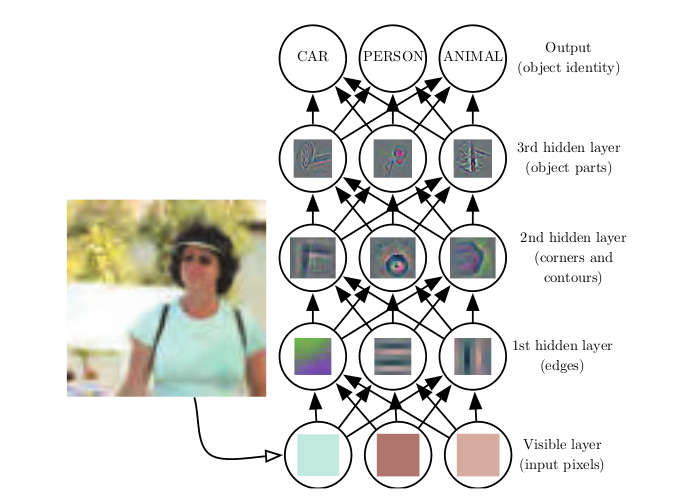
\includegraphics[scale=0.5]{figures/image-classification.png}
    \caption{Image Classification Deep Neural Network. Original source: \cite{goodfellow2016deep}}
    \label{fig:dnn_classify}
\end{figure}

\section{Convolutional Neural Networks}

Convolutional Neural Networks (CNN's, sometimes called Convnets), introduced by LeCun around 1995 \cite{lecun1995convolutional} are a specific and modern neural network architecture. This architecture specializes in working with data which has spatial or grid-like relationships. Some examples include images (e.g. two dimensional grids for grayscale image data), time-series data (which can be seen as a one dimensional grid), or other sequence data. Convolutional neural network have found their way into many successful implementations and are as of today one of the most common (and modern) type of deep neural networks. The name convolutional neural network comes from the mathematical operation of convolution, and it implies that a neural network uses this operation for some operations (feature extraction). To define formally: "Convolutional networks are simply neural networks that use convolution in place of general matrix multiplication in at least one of their layers." \cite{goodfellow2016deep} Besides convolutions, some other operations are usually required for a successful CNN implementation, like for example pooling, which will be explained later. Convolutional neural networks take inspiration from the animal world. Specifically, some animals have developed parts visual cortexes where information is processed in way that the surrounding information is also taken into consideration. In the case of image processing, for example, this simply means that we no longer look at the image pixel-by-pixel but rather we look at groups of neighbouring pixels. This is a powerful concept in learning and generalization in modern neural networks.

\subsection{Convolutional Kernels}

Convolutional Neural Networks can have many convolutional kernels or convolutional filters. These kernels are used for calculating the convolutions and in them the weights (knowledge) is stored similar to the weights on the synapses of fully-connected neural networks. Here, we explain briefly what are convolutional filters, what is the operation of convolution and what is the motivation behind using convolutions in neural networks.

In the most general mathematical terms, convolution is an operation on two functions of a real-valued argument. In deep learning the term convolution is used when we want to specify that we are using a convolutional operation to process the input data or some hidden layer data. The correct terminology for two parameters to the convolutional operation are: the input and the kernel (or filter). The output of the operation is often called a feature map (map which shows where are some features detected). The data processed in the case of CNN is always a multi-dimensional array (tensor of usually three dimensions: width, height and depth -- for a color image input depth is the color channels) which is used as an input parameter to a convolutional operation and another tensor called kernel. 

The easiest way to explain the convolutional operation in CNN's is by a simple example. In image processing operation of convolution means that a smaller sized image (kernel) is slid over the larger input image. The operation computed during the sliding is a simple element-wise multiplication. If a feature image matches a part of the input image the output of the operation will be a non-zero number in the resulting image (feature map). It is important to say that we do not define convolutional filters, they are learned through back-propagation like other learnable parameters in neural networks. One example of convolutional processing can be seen in Figure \ref{fig:conv}.

\begin{figure}
    \centering
    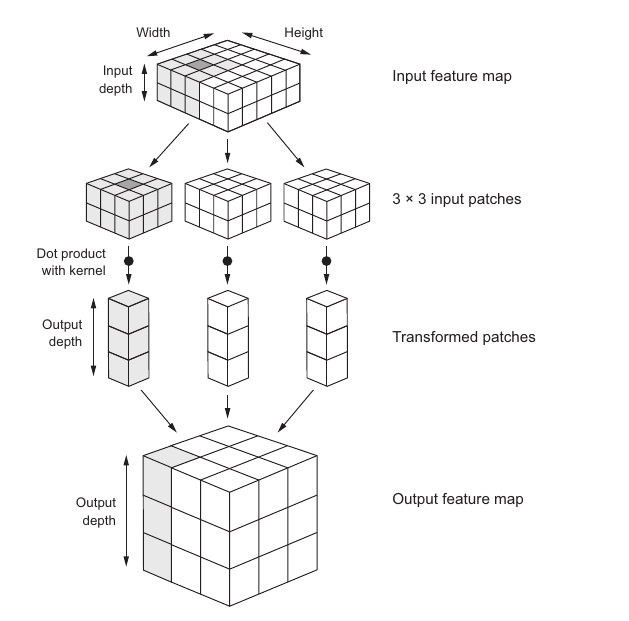
\includegraphics[scale=0.5]{figures/conv-chollet.png}
    \caption{Example of a convolutional operation on input data. Taken from \cite{chollet2018deep}.}
    \label{fig:conv}
\end{figure}

The main difference between a densely connected layer and a sparsely connected convolutional layer is that the dense layer learns global patterns in input data (e.g. pixel data in an image) and the convolutional layer learns local patterns (e.g. patterns found in images -- edges, shapes etc.).

This approach gives CNN's two interesting properties: patterns they detect are translation invariant (it does not matter where they are in the input data) and they can learn spatial hierarchies of patterns (first conv. layers learns local patterns, the next one learns larger patterns etc. like we described in the previous section).

Convolutional layers in neural networks have two key parameters: size of patches extracted from the input (usually squares of small dimension: e.g. 3x3 or 5x5) and the depth of the output feature map (defined by the number of convolutional kernels). Other than these parameters, we can also define padding (adding data around the input data for compatibility reasons) and stride. Stride defines how a convolutional filter is moved through the input data -- how large is the movement step. 

Another important parameter is downsampling or pooling. We use pooling (usually max-pooling) to reduce the size of the output convolutional feature map. These feature maps are propagated through many convolutional layers and it can be computationally expensive to process them in full. That is why we opt for the down sizing them by using the max pooling operation which only keeps maximum values from parts of the feature map output. Another benefit of this operation is better generalization -- e.g. to classify an object it is not important where it is in the image, but whether it is present anywhere on the image.

Convolutional Neural Networks can be and are used for many other image-related and other tasks. Apart from the textbook example of image classification they can be used for image segmentation \cite{yang2017suggestive}, object detection \cite{redmon2016you}, object detection in videos \cite{ciaparrone2020deep}, video classification \cite{karpathy2014large}, image superresolution \cite{dong2015image}, sentence classification \cite{joulin2016bag} and many other tasks.

\subsection{ImageNet}

ImageNet Large Scale Visual Recognition Challenge (ILSVRC) \cite{deng2009imagenet} is a widely known competition in object detection. A dataset of billions of images and 1000 classes is provided and different research teams compete every year to improve upon state-of-the-art results. ImageNet challenge became widely known around 2012 when Krizhevski et al. \cite{krizhevsky2012imagenet} demonstrated that CNN's can be used successfully for this use case. The initial CNN model they demonstrated may be simple in today's terms, but it brought down the state-of-the-art error rate of 26.1 percent to a new record of 15.3 percent -- a huge leap forwards. Since then ImageNet challenge is dominated by neural network models, and today's state-of-the-art models have top-5 errors rate as down as 3.6 percent.

Another important consequence of the ImageNet challenge and the reason we mention it here is that it introduced researchers to parameter sharing and transfer learning. For the model to be validated it had to be shared, meaning that it's parameters were publicly available. Most importantly, convolutional kernels were shared and they could be freely used for other tasks. It is quite common today to use pre-trained (meaning frozen, constant) convolutional layers in an image-related neural network. As the ImageNet models are trained from all publicly available images on the Internet, the convolutional layers are incredibly valuable as they contain almost every imaginable image feature there is. In one of our negative models, transfer learning is used as an important step in the training process. 

\section{Recurrent Neural Networks}

Recurrent neural networks (RNNs) introduced by Rumelhart et al. in the 1980s are a type of neural network used for processing sequential data. \cite{chollet2018deep} As convolutional networks are specialized for processing of grid-like inputs, such as images, a recurrent neural network model is specialized for processing sequences of values. As Convolutional Neural Networks can readily work with large images by looking only at their parts, RNNs can usually work with long (or infinite) sequences. Where feed-forward fully connected networks would fail with large sequences limited by their architecture, these specialized models are made to look at parts of sequences in order making them fully scalable. Also, like some CNNs can process images of variable size, RNNs can be made so they can process sequences of variable length.

Jumping from classic fully connected networks to recurrent models requires a special paradigm: parameter sharing across different parts of the model. Parameter sharing makes it possible to apply the neural network model to examples of variable form (different length) and generalize across them. If we are to have separate parameters for each value in time, we could not generalize to sequence lengths not seen during training. Sharing is important also to remove positional correlations in the data. Sentences "I lived in Coimbra in 2020." and "In 2020, I lived in Coimbra" have the same meaning, even though through the eyes of an algorithm they are completely different. Similarly how CNN models are invariant to feature positions in images, we want our sequence models to be invariant to term positions in them. Some 1-D CNN models can be used for sequence models but in comparison to RNNs they are shallow -- they can only look at neighbouring parts of the sequence, without memory.

In practice recurrent neural networks are implemented so they accept in addition to the input a hidden state input which is usually the output of the last time step.

Recurrent networks can be split into many different categories, to name a few common ones:

\begin{enumerate}
    \item Recurrent neural networks producing output at every time step, and have recurrent connections between hidden units
    \item Recurrent neural networks producing output at every time step, and have recurrent connections only from output of a step to the input to the next step (like in the example above)
    \item Recurrent neural networks with recurrent connections between hidden units that accept the entire sequence and then produce a single output value
 
\end{enumerate}

\subsection{Modern RNNs, memory and attentive models}

In this section we will discuss some of most important sequence models.

One important RNN model to mention is the Sequence-To-Sequence model (seq2seq \cite{sutskever2014sequence}). This model uses an encoder-decoder architecture to map one sequence to another. The sequences do not have to have same length. This model is used very successfully for Neural Translation Tasks.

One issue that recurrent neural networks have due to the vanishing gradient phenomena \cite{hochreiter1998vanishing} it is very difficult for them to take into consideration states from many time steps before. Two successful approaches to this problems are the gated recurrent unit (GRU) \cite{chung2014empirical} model and the long short-term memory (LSTM) \cite{hochreiter1997long} model. Both of these architectures use gates or self-loops to produce paths where gradients can flow for a long period of time. LSTM model especially has found great success in tasks like unconstrained handwriting recognition, speech recognition, handwriting generation, machine translation, image captioning and parsing. \cite{goodfellow2016deep}

Neural networks are very good at learning implicit connection in the data, but they lack in the simple task of memorizing of facts. This is due to SGD (stochastic gradient descent) requirement of many presentation of some input before it can be stored in a way in the network parameters. Even stored, the input will not be kept with high precision. Human beings are known to memorize facts though a "working memory" system (\cite{graves2014neural}). The need for a model that can process information as a sequence of steps (recurrent models) was clear and in \cite{weston2014memory} Weston et. al. introduced memory networks that include a set of memory cells. Memory networks, at first, required supervised signal to know how to use their memory cells, but in \cite{graves2014neural} Graves et. al. introduced Neural Turing machines \cite{graves2014neural} which were able to learn whether to write or read data from memory cells without supervision. This allowed self-contained end-to-end memory training with the use of content-based soft attention mechanism. This attention mechanism has become standard way of introducing memory to recurrent neural network models.

\section{Generative Models}

Even though artificial intelligence and specifically machine learning is mostly used on existing data to find hidden patterns and meaning, it was always known that with some modification, machine learning algorithms can be used to produce new, unseen data. Deep neural networks have been used for many generative tasks such as text generation, image style transfer, image generation etc. \cite{chollet2018deep}

Our languages and artworks all have hidden statistical structures. Learning these structures is what deep-learning algorithms excel at. These models can learn the statistical latent space of images, music, and stories so they can sample this space and create new works with many of the existing characteristics found in training data.

For text generation, recurrent neural networks which are used for sequence modeling as we already mentioned, can be used not only to predict or classify text but rather to write it. Working with generative RNNs can be generalized to any sequence data, not just text. LSTM networks have been used with great success to generate music, for example (e.g. Magenta \cite{roberts2018magenta}). The process of generating new sequence data is quite straightforward. First, we train a RNN model which is used to predict next items in a sequence e.g. next letter in a sentence. Then, with the model trained we give it some initial starting text (often called conditioning data) and ask it to generate the next value. Then we add that value to the starting text, and repeat the process many times. The loop allows us to create sequences of unlimited length. In sentence modeling, RNN models learn from human written sentences and are able to produce very coherent and meaningful sentences. It is very important to mention sampling strategy. It is not a good idea to use greedy sampling as in normal RNN prediction models. Greedy sampling is a sampling strategy where in every time step the best result is taken. If we were to use such strategy with generative models, we would get repetitive and meaningless sequences. If we introduce stochasticity or randomness to the process, we usually get much better results.

Another area where generative models excel is image processing. DeepDream \cite{mordvintsev2015inceptionism} is an artistic image-modification experiment developed at Google. It quickly became an Internet sensation because it generated some very weird-looking images given an image output. The weirdness came from various artifacts taken from convolutional layers of a CNN trained on the ImageNet dataset. It used reverse convolutions, and gradient ascent on the input image in order to maximize the activation of a specific filter (or many filters, entire layers even) in upper layers of the CNN.

\begin{figure}
    \centering
    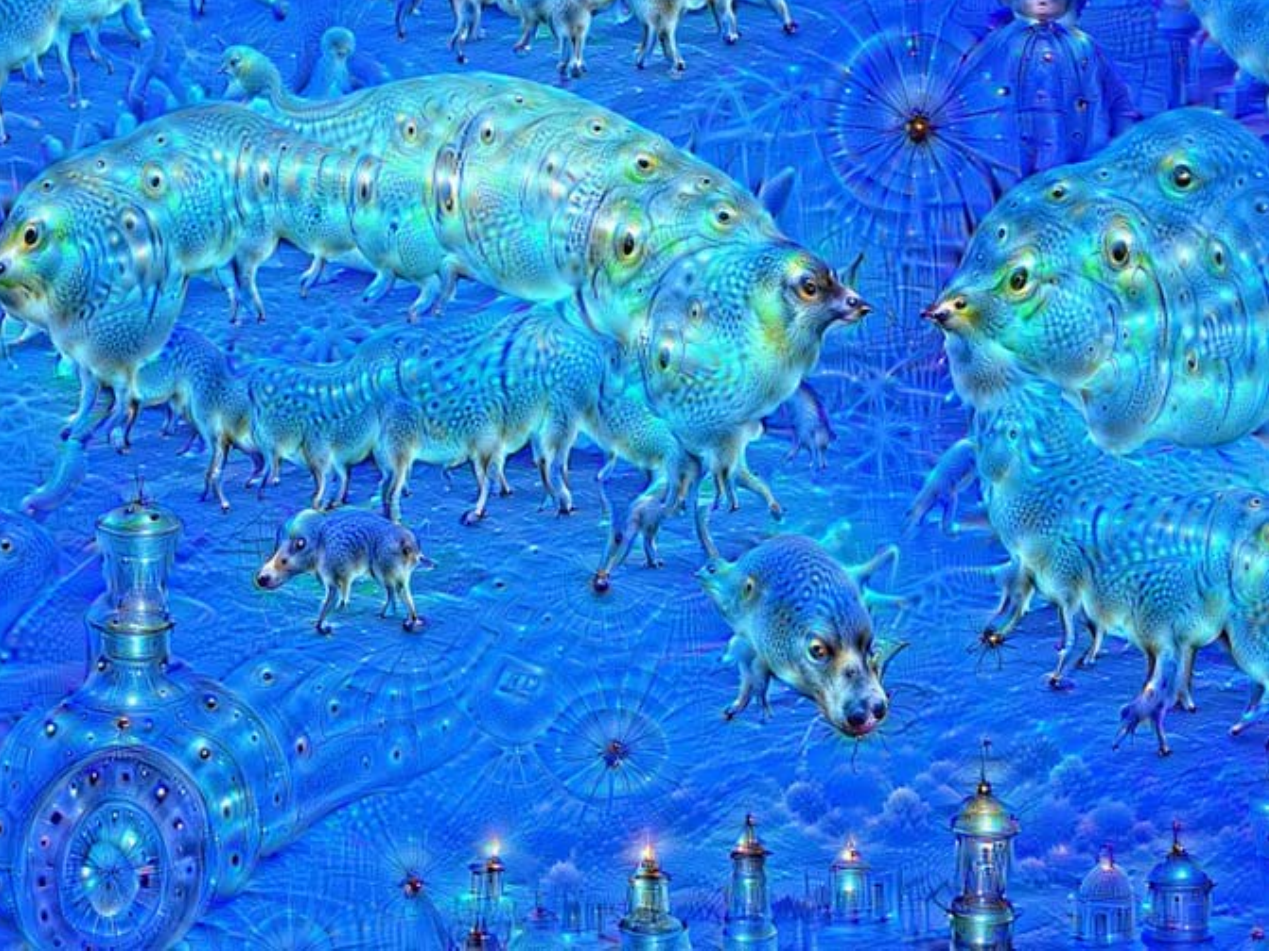
\includegraphics[scale=0.2]{figures/deepdream.png}
    \caption{Example of a DeepDream network output image. Taken from \cite{chollet2018deep}.}
    \label{fig:deepdream}
\end{figure}

Another image processing generative network which received major praise was the Neural Style Transfer \cite{gatys2015neural} algorithm. This algorithm can be used to transfer artistic style from one image to another while preserving content. Style, in this context means textures, colors and visual patterns found in images, while content represents the structure of an image. The style transfer is achieved by implementing a specific loss function and minimizing it, like in almost all neural network applications.

The loss function would look something like this:

\begin{multline*}
loss = distance(style(reference_image) - style(generated_image))\\
+ distance(content(original_image) - content(generated_image))
\end{multline*}

In this formula distance function is a norm function such as the L2 norm, content is a function that takes an image and computes a content representation, style is a function which does the same for style. Minimizing this function causes both the style and content values of two images to be closely related. The interesting part of this algorithm of course is how to define the content and style loss functions. To put it simply we can use convolutional layers at various depth to extract image representations. The depth is very important because we know that earlier convolutional layers contain low-level local information about an image, and the deeper layers contain more abstract global information. The style loss has a bit more additional complexity: style can be captured at all layers in the network, and that is why Gatys et al. (the original Neural Style Transfer authors) suggest usage of Gram matrices which are the inner product of feature maps in a convolutional layer. This inner product can be understood as a map of correlations between layer's features.  These feature correlations contain the statistics of the patterns of a particular spatial scale, which empirically were found to be the textures in an image.

\begin{figure}
    \centering
    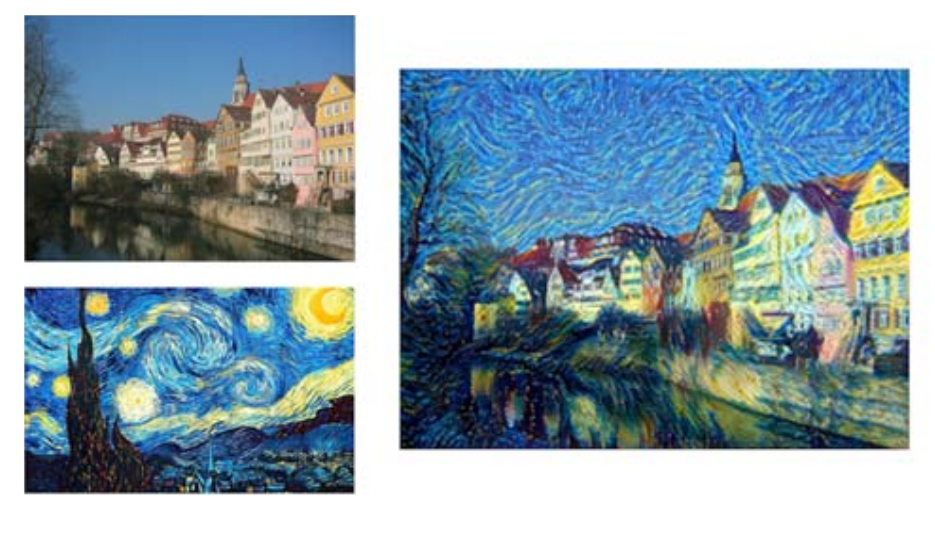
\includegraphics[scale=0.45]{figures/nst.png}
    \caption{Example of a Neural Style Transfer application. On the top left we have an input image -- a photograph. On the bottom left we have Van Gogh's Starry Night, used to extract style. And on the right we have the resulting image, content from the input image, style from the Starry Night. Image taken from \cite{chollet2018deep}.}
    \label{fig:nst}
\end{figure}

Another popular generative method is the Variational Autoencoder (VAE) \cite{chollet2018deep} model. Autoencoders are a special type of neural networks where the input and the output are identical. The benefit of these models comes from their architecture. All autoencoders have such structures that the input is reduced in size until one point in the network and then increased in the next. These two parts of the model are called the encoder and the decoder and the middle point in the network is called the bottleneck. When a model like this is trained it is forced to learn a compressed representation of the input so it can use that representation to decompress it and produce that input again as the output. Autoencoders can also be used for clustering \cite{chollet2018deep}, anomaly detection \cite{an2015variational} and many other unsupervised tasks -- in which traditionally neural networks are not used. 

Autoencoders are also generative models. \cite{kusner2017grammar} \cite{pu2016variational} If we take the decoder part and feed it some random inputs, we will get an output of some sorts which would be similar to some parts of our training dataset. This way of sampling from latent space of images for example to create new images or modify existing images is one of the most popular and successful applications of generative models today. We mentioned latent space and we define it as a low-dimensional vector space where any point can be mapped to a realistic-looking image. When we create this latent space we can sample from it, deliberately or at random and the output becomes a previously unseen input (image). VAEs learn latent spaces that are well structured where specific directions in the multidimensional vector space encode meaningful variations in data. If we train a VAE with a dataset of portraits for example, one such direct would be hair color or whether the person in the image is smiling. \cite{hou2017deep} At the end we need to emphasize differences between traditional autoencoder models and the variational autoencoder model mentioned here. VAEs differ from normal AEs in that we impose various constrains on the latent space definition so we force the model to learn better representations of features found in input data. For example we can limit the latent space to be low-dimensional and sparse, forcing the model to learn better. When comparing latent spaces of normal AEs and VAEs it is apparent that VAEs have better defined structure. This is because VAEs in addition to compressing input data into a fixed point in the latent space also turns the data into parameters of a statistical distribution (mean and variance). This means we assume that the input data has been generated by a statistical process and that the randomness of the process should be considered during encoding and decoding. The mean and variance parameters are then used to randomly sample one element of the distribution to decode that element to the input to the model. The randomness of this process improves both the latent space structure and continuity and the robustness of the whole process.

\subsection{Adversarial Learning}

Generative Adversarial Networks (GANs) which were introduced in 2014 (Goodfellow et. al.) \cite{goodfellowexplaining} are another generative neural network model. They also can learn latent spaces of images (or other data) similar to VAEs. GANs can generate fairly realistic synthetic images by forcing them to be statistically indistinguishable from the real images.

Easiest way to explain generative adversarial networks is to imagine someone trying to forge a Picasso painting. In the beginning the forger will perform poorly because lacks authenticity. However the forger will then mix his own work with actual Picasso paintings and show them to a trained art dealer. The art dealer will tell him what he thinks about the pictures and how he was able to distinguish the real pictures from the fake ones. He will also provide information about what he looks for in authentic Picasso pictures. As this process is repeated, the forger will use this information to become better and better at forging the pictures until the art dealer cannot distinguish between actual Picasso paintings and the forger created ones.

This is exactly how a GAN works. It is joint model of two networks: a forger (generator) network and an adversary network. Hence the name generative adversarial networks.

The generator network takes a random vector (random point in the latent space) and produces a synthetic image. The adversary network takes as input image and predicts whether the image is from the training set or from the generator network. The generator network is trained to fool the adversary network, as it evolves and creates more and more realistic looking images. The adversary (sometimes called discriminator networks) meanwhile judges the work of the generator network.

GANs and other adversarial learning methods have found their use not only for generating data but also for testing the robustness of trained neural networks. They can be used for input modification (such as perturbations or occlusions) which are then use to trick the trained network into a wrong classification output. Usually, the goal is not just to modify the inputs so it wrongly classified but also for that input to remain recognizable to the human eye. The modified input image can look entirely normal but to be wrongly classified by a performant model. This is called an adversarial attack and we will focus on this topic later in this manuscript.

\subsection{Deep Reinforcement Learning}

Another great success in the field of Machine Learning and specifically Deep Learning was the introduction of deep reinforcement learning algorithms. In the scene set, an agent enabled with a powerful neural network model must learn to perform some task by trial and error, with any guidance from its human operator. DeepMind demonstrated that this type of learning algorithm can be taught to play old Atari games, reaching and surpassing human levels of play. \cite{mnih2013playing} Deep Reinforcement Learning models also made headlines when AlphaGo \cite{silver2016mastering}, a trained agent playing the board game Go, was developed and defeated world champions on several occasions. Another area where these algorithms have found great success is in robotics and also in self-driving cars \cite{dosovitskiy2017carla} -- a very popular field nowadays. We will cover deep reinforcement learning in more detail later in this manuscript.

\section{Future of Deep Learning and Towards Artificial General Intelligence}

This section contains some authors speculations about the future of Deep Learning and its uses.

Moving forwards towards new chapters in the field of Artificial Intelligence we can expect that Deep Learning will move away from model only performing pattern recognition and can achieve limited local generalization. We will need to develop model able to develop abstractions and reasoning while achieving extreme global generalization. Current AI programs that are able to reason are mostly hardcoded by their programmers, even in most advanced Deep Reinforcement Learning approaches. In DeepMind's AlphaGo, for example, most of the learned intelligent behaviour is designed and coded by expert programmers (e.g. Monte Carlo Tree Search) and learning from data only happens in part of the system (value and policy networks). In the future AI systems should be able to "code themselves" without human involvement. 

The current neural network models are limited by their programming to be a set of geometrical operations on an input vector. A model able to freely modify its own code with a set of defined programming language rules would be able to achieve much better results in all scenarios. In a way, computer programs could be replaced with machine learning models which are self-programmed. One interesting research field related to this is neural program synthesis. \cite{bunel2018leveraging} Program synthesis consists of automatic generation of simple programs by employing search algorithms (even genetic, as in genetic programming) to explore a large space which contains all possible programs. The search stops when a program with a matching specification is found. The specification is often given as a pair of input-output pairs which is of course reminiscent of machine learning. The difference is that instead of learning parameter values (weights) in a hardcoded neural network we generate new source code in a discrete search process. 

These new programs won't be differential like the hardcoded neural network models of today. Therefore backpropagation will need to be replaced with a more suitable method. Whether that is genetic algorithms, evolution strategies, alternating direction of multipliers \cite{wahlberg2012admm} or other method \cite{jakovetic2014fast}, some things will need to change. Gradient descent will probably stay because the gradient information will always be useful for optimizing differentiable parametric functions.

Of course, all Deep Learning models will eventually become portable, in a way that they can be trained and ran or various mobile hardware. We are already witnesses of mobile chip development specifically with neural network image processing in mind. Many of the mainstream machine learning frameworks and libraries already support running models on mobile phones and other portable computers. Different concepts like network compression, pruning and quantization \cite{choi2016towards} exist today to ease the transition of resource-intensive models to relatively weak but increasingly stronger devices we carry today.

In short, this perpetually learning model-growing paradigm can be interpreted as AGI (artificial general intelligence) where models can learn and learn what to learn and how to learn. This is not something easily achievable and with no clear way of doing it, it will be years before we are close. When done, however, our lives will change significantly.

\section{Modern Neural Network Concepts}

In this section, we briefly go over some of the state-of-the-art concepts and research taking place in the field of Deep Learning.

\subsection{AutoML}

Automatic machine learning or AutoML \cite{he2021automl} is a fairly new concept in the field of Machine Learning. Today, most of the machine learning architectures are still defined by their human operators. In the future, and today already we have some methods of unsupervised architecture optimization. This allows the model to adjust not only its parameters but its architecture as well. Some problems, it has been shown, can be solved better and easier with a specific architecture which is hard to conjure. 

Going further, the main job of a deep learning expert nowadays is to structure the training data and come up with a good set of hyperparameters and a good architecture for a specific problem. Needless to say, this is a lot of work. With AI's help several steps of this process can be automated. The data preparation (or data cleaning, as it is often called) is very difficult to automate, because it often requires domain knowledge as well as a clear, high-level understanding of what is to be achieved and in what way. Hyperparameter tuning, however, is a different story. It can be seen as a simple search procedure, or a trial-and-error process. In this case, we already know the ideal outcome which is the minimization of the loss function in training. But we want to find the best hyperparameter values. It is possible today to use an AutoML framework, and set it up to find best hyperparameter values for a certain problem. The most basic AutoML implementations would define arrays of possible hyperparameter values and try various combinations of them. The parameters can be basic values such as learning rate or momentum but they can also be more complex like for example number of layers or number of units in a hidden layer etc. One good example of this method is NAS or Neural Architecture Search \cite{elsken2019neural} method.

\subsection{Transformers}

Transformers are a deep learning model introduced in 2017. \cite{vaswani2017attention} They are used specifically for sequential data similarly to recurrent neural networks. Unlike recurrent neural networks Transformers do not need to process the input data in order making them easier to parallelize with loss in model quality when compared to state of the art RNN models like LSTMs for example. This means that larger and more complex models are possible to train and use, and also that larger amounts of data can be used for training. One such use case is of course in text processing where Transformers are currently state of the art models used for various tasks like machine translation, document summarization, document generation, named entity recognition, and others. They can also be used for other sequential data like for example biological sequences. One research group even showed that a specialized transformer architecture can be used for playing chess. In 2020, many language models were made available by leaders in the Natural Language Processing field. Most notable include: GPT-3, GPT-2, BERT, XLNet, RoBERTa and others. These models attracted lot of attention because of their ability to generate stories or volume of texts almost indistinguishable from human written text. 

Speaking of attention, it is important to mention it here. In the paper "Attention is all you need" \cite{vaswani2017attention} where Polosukhin et al. introduce Transformers it is shown that attention is a very important parameter in neural network models used for sequential data. As we briefly mentioned in previous sections regarding recurrent models, today's gated recurrent models (LSTM, GRU, etc.) use gates to simulate memory. Attention mechanism not only allows the RNNs to remember many previous states (solving the problem with older RNN models) but to distinguish what previous states or previous information is important. In a neural machine translation task, for example, it is obviously important to look at entire sentences for translation instead of just the previous time step. The authors of the mentioned paper use attention-like method but without the requirement for sequential processing of data, allowing parallelization. Lastly, transformers are still an encoder-decoder architecture similar to other models we mentioned in this manuscript.

% https://en.wikipedia.org/wiki/Transformer_(machine_learning_model)

\subsection{Federated Learning}

As mobile devices and sensory IoT devices become more and more involved in machine learning workloads the need for decentralized training or collaborative learning is increasingly apparent. Federated learning \cite{li2020federated} is a machine learning technique that trains a model across multiple devices. These devices can vary in architecture, power or other capabilities. One specific point is that in federated learning there is no single centralized data store where the training data resides. It is rather split into chunks and every device (node) has limited amount of information for training. In other words, nodes rely on each other for a performant model. This is very useful in scenarios where many devices gather data (e.g. sensors in factories), because that data can be processed immediately. Another benefit is from the data sharing standpoint, as the data does not necessarily need to be shared across various devices addressing critical issues such as data privacy, data security, data access rights and access to heterogeneous data.

There are many ways in which federated learning can be implemented. One closest to other topics in this manuscript is of course the decentralized deep neural network model. In this scenario local models are created and trained with local data samples and parameters such as weights and biases of the model are then shared with other nodes. Other nodes choose how to use the knowledge shared with them, usually this knowledge (parameters) is averaged with local parameters and then taken into consideration. Federated stochastic gradient descent (FedSGD) and its generalization Federated averaging (FedAvg) are commonly used.

It is important to mention that federated learning is not the same term as distributed learning. Distributed learning has a different purpose: to train a single model across many devices. The single model is often too large for a single node or the training time is too long because of a large dataset. That is why we can use a set of computing nodes which are used for their processing power.

Federated learning technique is used a lot for online learning (additional training for existing models) as well as for critical systems where privacy is a priority. Some examples include self-driving cards, Industry 4.0 use-cases (smart manufacturing processes), medicine and others. \cite{arapakis2019towards} Federated learning is also accelerated by recent hardware developments both in ARM chips and in network infrastructure like 5G broadband networking.

\chapter{Goals and contributions of this thesis}

In this chapter we briefly present the reader with goals and motivation as well as contributions and the realization plan of this PhD thesis. 

\section{Goals and motivation}

The main goal of this thesis is to explore negative learning application for Deep Learning models. Negative learning is present in every-day life and it is a known term in psychology and behaviour studies. With our research we are trying to create a bridge between symbolic understanding of patterns and the innate low interpretability of deep learning models. In other words, we are trying to extract or, more precisely, deduce additional knowledge from existing data, similar to what would a human do if presented with a certain task.

Another goal of this thesis is to define and implement negative deep learning models so others can benefit from our work and use these models for various tasks. We will define several negative models from negative convolutional neural networks, synergy ensemble positive-negative networks, true negative networks (e.g. negative Siamese networks) and negative agents.

For some of these models the goal is evaluate them in-depth in some use cases where we hope they would perform well. For negative and synergy models the goal is to have better performance with regard to robustness in difficult scenarios such as partial inputs, occlusions, adversarial attacks etc. 

For other models the goal is to evaluate the possibility of training and using them with negative learning in mind.

\section{Contributions}

The contributions of this PhD thesis can be divided in several categories.

Broadly and most importantly, the introduction of negative deep learning as a new paradigm in Machine Learning research is a great contribution to all researchers in the field. 

Our detailed in-depth explanations, examples and implementations of the presented models is also a great contribution to research. We also provide reproducible and tested environments in which our models can be tested and our results validated. Significant time was spent on various in-depth experiments with our presented models so that many questions from researchers wanting to experiment with our models are immediately answered. For example for our negative models which learn to classify on negative features we already experimented with different activation functions, layer freezing, transfer learning, fine-tuning, convolutional layer inversion and other approaches. For our negative reinforcement learning agents we already provide one example environment where these or similar agents can be tested.

We also provide full source code and implementations for all the models and experiments presented in this thesis which we believe is a necessity in modern research.

\section{Realization plan}

The realization plan and general development of the models and experiments in this thesis closely follows the actual contents of the thesis.

First, we provide a short introduction and overview of the field necessary for defining negative deep learning models. After that we will discuss possible implementations and provide some examples and their application. In the next part we go in-depth with our first negative learning model which can classify instances based on their missing features. We present all the different experiments that were performed and the results. In the fourth part we discuss in-depth the Synergy model, another negative deep learning model. Then, we examine what we call "true" negative deep learning models, models which only learn from negative data. The main focus is on our own: a negative Siamese Triplet Loss neural network. Finally, in the last part we also discuss how negative deep learning can be used in agent environments and provide examples for both the agent and the environment.

\section{Note on Related Work sections}

During the production of this PhD thesis it was decided that the related work discussion should be included in specific parts of the manuscript. Our feeling is that this is a more natural approach as this thesis aims to cover a wide variety of fields of Machine Learning research. Therefore, a singular related work section does not exist but it rather split into parts which follow the natural flow of the document.

\part{Negative Learning}
\chapter{Introduction to Negative Learning}

In this part of the manuscript we define negative learning as a term taken from cognitive psychology and we describe ways of introducing it to the field of Deep Learning.

Negative learning in psychology \cite{mcleod2007bf,staddon2003operant} can be defined in many ways. One way to define it is learning with a negative reward or a penalty. This approach can be directly applied to agent-based algorithms like for example, Reinforcement Learning algorithms. Learning with a negative reward or penalty is described so that an agent can be penalized for its actions if they are deemed inadequate. For a self-driving car for example some actions can be seen as positive and some can be seen as negative. Positive action would be for example stopping at the stop sign, while a negative action can be crashing or speeding. When training these agents, it is necessary to do so with both positive and negative examples of behaviour. This approach takes inspiration directly from human behaviour. Children for example are often disciplined when behaving in a inappropriate way.

An algorithm which only uses negative samples for learning, hoping that if it knows all the actions which should not be taken, will be able to deduce the correct (positive) action, would be called a negative learning algorithm. It is difficult to say whether it is a good approach for an algorithm to only learn using negative samples. We will see in later sections that this is possible.

Negative learning can be defined also in the realm of two large sub groups of machine learning problems: classification and regression.

In classification tasks a machine learning algorithm is needed to classify certain input data. We differentiate binary (two-class) and multi-class classification. The algorithm outputs to which class from a predefined set of classes the input belongs to. It does so based on its features. During training many examples of the input and output data are presented to the algorithm. It learns and changes its parameters so it can classify all the provided input-output examples. Negative learning in this case can be defined in several ways. We could ask for example to what classes the input date does not belong. Another example would be if we asked what features need to exist so we know the input data does not belong to a certain class. We will visit these questions (and implement them) in the following parts of this manuscript.

Similarly, in a regression task a machine learning model is tasked to output a real numbered value for a certain set of inputs. A negative learning model in this case would be able to tell us not what the expected output for a certain point is, but rather what scope of output values is not expected. We could also model regression tasks as classification tasks, if we were to discretize the data of course.

There are other ways to define negative learning, but in this manuscript we will focus on the three mentioned problems here: problem of classification, regression and agent-based environments.

\section{Reasoning and possible benefits of Negative Learning techniques}

There are many reasons why one would need to use techniques we describe here. 

For one, positive examples may be unavailable during training. If we have only negative examples for the model to learn from we need a model capable of understanding that it is dealing with negative information.

Another reason is for increased robustness. As we will discover later, negative models in some scenarios are proven to be more robust than their positive counterparts. Robustness here means that the model will have same or increased accuracy in difficult situations. These difficult situations can be defined as situations where traditionally machine learning models have issues: missing data, partial data, adversary attacks etc. Negative samples can be seen as additional information available for our model. This additional information can be very useful in difficult scenarios when a model is not certain. 

One more reason is increased performance of the models. Similarly to robustness if the models use this additional negative data in a correct way, they can converge quicker or have increased accuracy, precision or other important metrics.

We will mention more use cases specifically for Negative Deep Learning in the next chapter.

\section{Policy-based algorithms and Negative Learning}

Policy-based algorithms are a natural contender for negative learning. As mentioned earlier, policy-based algorithms (e.g. reinforcement learning algorithms) learn a policy function based on which an agent behaves in an environment. This policy function is learned in an iterative process of trial and error where the agent tests various actions that are possible and how they affect the environment. This policy function depends largely on the reward/penalty function where the agent is given a numeric value denoting a positive (reward) or a negative (penalty) outcome of the last action performed.

Negative learning in the case of policy-based algorithms can be seen as using only negative values for the reward/penalty function. The policy learned in this way would only have negative knowledge in its definition. In other words, the agent would only know what not to do in certain situations. The action chosen would be a randomly selected one, but the chosen action would certainly not be an action which the policy function knows to incur a penalty. This is one of the purest forms of negative learning, where the agent only knows what actions are not to be taken.

\section{Negative Learning in other algorithms}

In the task of binary classification, literature often separates the date into two categories: positive and negative data. Positive meaning the data which has a "True" value and negative meaning data with a "False" value. It is easy to define negative learning as learning from only the negative parts of the data. One has to be careful in these scenarios as overfitting is highly probable for various models. Overfitting is a case in machine learning when a model highly favours one output class in a classification task. If we are only to train with negative data, it is highly likely that our algorithm would learn to always output negative outcomes even when data for a positive outcome is given. Negative Deep Learning as we will see later makes more sense for multi-class classification problems but can also be used in certain ways for binary classification.

One more interesting contender for negative learning is in the problem of anomaly detection. In anomaly detection tasks, an algorithm is trained so it can recognize certain irregularities in data. These irregularities are called anomalies and can be defined as anything which differs from the normal data that the model saw during training. However we can also define these models in reverse. 

In anomaly detection problems algorithms (such as autoencoders) are trained on filtered data which does not have anomalies. In a way the model is forced to learn and memorize normal data so that later on it can recognize when anomalous data is given. Negative learning version of this algorithm would be to train the model on only the negative data (or anomalies). That way an algorithm would learn how anomalies look like and would learn to recognize them among normal data points. Some literature defines this as a traditional positive learning approach, so it is very interesting that traditional anomaly detection can be seen as a negative learning method.

\chapter{Negative Deep Learning}

In this chapter we begin to define negative deep learning methods and provide an overview of possible implementations and use cases. We also provide several necessary definitions before we move to concrete examples in following chapters.

\section{Negative Deep Learning -- Introduction}

By the term negative deep learning in this manuscript we consider all deep learning models, existing and newly-introduced here, which use negative data. Negative data can take many forms which we will discuss in later parts of the manuscript. Negative data can be, depending on the task at hand, missing data, inverse data, wrong data, noisy data, adversely generated data etc.

Negative deep learning models are special in that they can use this negative data as additional information during the learning process. These models use the negative data by employing special architectures and training processes (among other changes) so they can differentiate normal and negative data during training. The necessity and the benefits that we will see later are: increased robustness in different scenarios like partial input classification, adversarial attacks etc, faster convergence, possibility of fine-tuning of existing models and many others.

\section{Possible Models of Negative Deep Learning}

In this section we discuss several approaches to the negative deep learning model implementation. Some of these approaches will be described in great detail in the following parts of the manuscript.

\subsection{Missing Features}

One way of implementing negative deep learning is to use "missing features" in input sample. Term "missing" is not entirely correct as it is very rare that a feature is completely missing from an input sample, rather it is of low activation or low importance. All neural network models use high importance features to learn certain patterns in data. Low importance features (e.g. for a specific class) are also used, but in our negative learning models \cite{milovsevic2019classification} these features are deemed more important than the others. This allows the model to learn the data patterns not by looking at present, high importance features. The model learns from missing (negative) features in the data and it prioritizes them in the learning process. In a way our model is learning to deduce what pattern in the data should be recognized by looking at all possible features and those which are missing. This perhaps seems simply like a new approach to learning which will not have any benefits, but we have to think what happens in certain scenarios which are proved to be difficult for modern neural network. In partial input classification, the neural network model should be able to recognize patterns in inputs which are not whole or complete. This is where deduction is extremely important. If a human is shown a picture of an animal which has the majority of its contents masked or removed, by observing what features are missing we can eliminate many of the output classes. If feathers are missing, for example, we can certainly say that it is very probably that the image we are trying to recognize is not of a bird. This is what the classification based on missing (we will call them negative in the future) features models are trying to achieve.

\subsection{Partial Input Sample Training}

Similarly to CBOMF (Classification based on missing features \cite{milovsevic2019classification}) we could achieve similar results if we were to use partial inputs in training. In this way of learning the model is never shown an entire input sample during training, rather only some parts of the input samples. These parts can be obtained manually or for some problems (e.g. in astronomy) they are the only data available, as the whole data is difficult or impossible to obtain. By training the model on partial inputs, we force it to learn the patterns in much finer detail and we expect that the knowledge obtained in this way will also be applicable during testing and usage of the model, when larger or whole input samples are presented to the model. The "negativity" of this model comes from the fact that we can also use parts of the input samples to say what they do not represent. This is additional manual knowledge introduced artificially to the model. But, it is also possible to generate data like this automatically with Negative Output Learning.

\subsection{Negative Output Learning}

During our research for this doctoral thesis, a laboratory in South Korea started doing somewhat similar research to ours \cite{kim2019nlnl}. Their models and methods are vastly different than ours, but the goal is similar, to introduce negative learning to deep learning models as a new paradigm. 

One approach they examined and which we will also subject to research in our own way is the negative output learning. To explain it simply this is the purest form of negative deep learning and it can be formulated as follows: A neural network is presented with an input sample and which class it does not belong to. The process of choosing the new "negative" output class is simple: we choose a random output class, making sure it is not the positive "correct" one. The difference is in the learning process and the loss function. Rather than trying to minimize the loss function so the model always outputs which class an input sample does not belong to, we use gradient ascent to "pull away" from the negative class and towards some positive class. In the case of m-ary classification only one class is the positive one.

Our approach is similar, but without modifications to the loss function. We simply modify the model so it learns which input samples do not belong to a certain class. We also experimented with gradient ascent without modification of the loss function by transforming the dataset so that the output one-hot vector (in m-ary classification) is inverted so that the actual class has zero value and other classes have the value of one. We will see that these models work best when used in combination with traditional neural network models. This approach will be described in great detail in later parts of the manuscript.

\subsection{Ensemble Networks and upgrades of existing models}

In our experiments it was made clear that many negative deep learning models work really well on their own. However since the paradigm of learning changes greatly it is sometimes beneficial to use these negative models in conjunction with traditional deep learning models. This idea came from our first negative deep learning model, the CBOMF model. This model when compared to a normal model of same architecture shows increase in accuracy when testing on samples with parts missing or occlusions. However, we discovered that the accuracy increase was not absolute. In other words, our model learned to classify some new examples from the testing portion of the dataset, but also lost the ability to classify samples which the traditional model was able to classify. The number of these cases was smaller than the newly classifiable samples, but the increase in accuracy was not absolute. The best result would be of course, if our model was able to classify everything that the normal model can classify and then on top of that to classify new previously wrongly classified samples. One approach to this problem is to use an ensemble model of the two networks: positive and negative which takes inspiration from the Siamese neural network architecture. These models were named synergy networks \cite{milovsevic2019classification} and they will be discussed later in the manuscript.

\subsection{Agent Environments}

Lastly, negative models show promise in agent environments. The main problem for agent based deep learning algorithms (e.g. Deep Q-Learning \cite{mnih2013playing}) is that the environments are often noisy and it is difficult to deduce what action should be chosen in a certain point in time. By using negative models we could help the agent to immediately discard many of the wrong actions so that the chances of it selecting the correct action are greater. Also, in cases where there is no correct action, we want to choose the action which is less incorrect in the negative modelling type of thinking. These changes can be implemented with negative deep learning models, e.g. negative output learning models where the agent would have additional knowledge in every step which actions should not even be considered. Negative Deep Reinforcement Learning models will be discussed towards the end of this manuscript.

\section{Negative Deep Learning Use Cases}

In this section, after we introduced several ways of having negative learning in deep learning models, we discuss some of the use cases we discovered are compatible with our new models. New use cases are certainly to be discovered, in this section we only present those which are already tested with beneficial results.

\subsection{Neural Network Robustness}

Neural Network Robustness has become quite a hot topic in Deep Learning research, especially in the last few years. \cite{carlini2017towards} Neural networks, among other machine learning models, have been used for some time as a "black-box" type of solution for many different tasks. However in recent times, many uses were found in which neural networks perform critical, life influencing calculations and decisions. Therefore it is important that they have the same or similar performance to humans in difficult situations. When we say difficult situations, it means situations which were not encountered during training or testing of the models and in which humans usually perform much better than artificial models. One example we mentioned already is in partial image classification, where humans are usually able to classify even parts of the images and we want that same quality to exist in artificial neural network models.

\subsubsection{Object Detection and Image Classification with Occlusions}

Neural networks, and especially convolutional neural networks have been used very successfully in the field of computer vision. In computer vision tasks we perform image learning which allows us to detect classes to which the image belongs to, objects in images, different segments of an observed image (image segmentation), video processing and many other tasks. Since images are well structured two-dimensional (or three-dimensional for color images) arrays of pixel data, convolutional neural networks which work best with structured data perform very well. In fact, CNNs are still, since their inception, state-of-the-art algorithms in many image related tasks. 

Regarding negative learning and robustness in image related tasks, we will discover later on in this manuscript that several negative learning models exist which significantly improve performance in the case of occlusions (object behind object, or object behind mask), and partial inputs. If we present the models with additional negative learning information, they learn the image space better and are able to classify better in difficult cases, which are very present in the real world. One excellent example for this type of application is self-driving cars. A self-driving system in cars must be able to correctly recognize road signs even if they are partially obscured by other vehicles, trees and other common objects. This is where models which are resilient to occlusions are not just necessary but essential for safety. One similar example is in case of damaged or dirty camera lenses in self driving cars. The system should not stop working if the image is blurry or partially damaged, again the case for robust models.

\subsubsection{Neural Adversarial Attacks}

In recent years, many methods have been discovered in the field of Neural Adversarial Attacks. \cite{goodfellowexplaining} While some have been used for new applications previously thought to be impossible like Generative Adversarial Networks \cite{goodfellow2014generative}, some have also been used to show that neural networks are very sensitive models when it comes to adversarial attacks. An adversarial attack is an attack in which the input signal is modified slightly in a way that the model used to process it makes a mistake. For example, in image classification we can add noise to the pixel data of an image so it is wrongly classified by a highly performant model. Some of the most advanced modern approaches to adversarial attacks can even modify images in a minimal way so they still look the same to humans, while they are wrongly recognized by modern CNNs. Adversarial attacks can also be used for other types of networks, not just images. 

Adversarial Attacks are also important in critical systems, as they can be used by individuals with malicious intent. Therefore, we need to make models which are less susceptible to these attacks, and we will show that negative learning models presented in this dissertation are of better performance when compared to traditional neural network models.  

Depending on the algorithm and the openness of the model which is being attacked we define two large subsets of adversarial attacks, black-box attacks and white-box attacks. We will demonstrate performance of different negative neural network models on both types of the attack in further parts of the document.

\subsubsection{Black-box attacks}

Black-box attacks are one type of adversarial attacks used to fool neural networks into wrongly processing some data. Black-box type of attack got its name from the nature of the algorithm. To explain, this type of attacks is not aware of the neural network internal structure, weights and other properties. It only uses it as a black box. It makes different modifications to the synthetic input data (starting from random) to see what noise can be added so that the attacked model makes certain assumptions. Then that noise can be added to different real input samples, and they are wrongly processed then. 

\subsubsection{White-box attacks}

White-box attacks differ from black-box attack in that they have full knowledge of the attacked model and are using this information to directly influence the network so that it makes mistakes. White-box attacks have full access to the network parameters such as weights and biases. More importantly these attacks have access to the network during the calculation of the gradients. In most approaches, these gradients are then manipulated so the network makes the wrong prediction.

\subsection{Negative Neural Networks for Regression Tasks}

It is important to say that while we only mentioned classification tasks and the usage of negative neural network models in that regards, they can also be used for regression tasks. First way is if we discretize the output space so that a regression tasks is perceived as a classification task. But, negative models can also be used for regression tasks without modification. It is easy to think of what a negative sample would look like in a regression task. In regression task we have data pairs of input features and an output value. A negative sample would be different in that for a certain set of input features we would know what the output should not be. So our model could adjust its parameters so the output is pulled away from the given negative output. The uses for this type of models are quite similar to other use case we described already. For tasks where the output is unknown but we know what the output certainly is not we could incorporate additional knowledge in the form of negative samples which then can be used to improve our model performance. 

\subsection{Other uses}

Another important use which we did not mention so far for both classification and regression tasks is inclusion of fail-safes in the deep learning models. The main issue with many deep learning models used in critical systems is that it is discovered that in certain critical scenarios unseen during training (e.g. late emergency braking in self-driving cars) they perform poorly. The developers of these models than program fail-safes in the code which prevent the model from making these mistakes in the future. These fail-safes are usually hardcoded outside the models and are difficult to maintain. The inclusion of negative-learning patterns can be perceived as a type of fail-safe programming used to include specific scenarios into the deep learning models. The difference is that these samples are properly integrated into the models, and they do not differ in that way from other data used for training.

We mentioned already the type of synergy negative learning model where two models are used in parallel to process some data with increased robustness. It is important to state that the synergy model we define in this manuscript can be used with any existing CNN (or other type of model). This is important from an integration standpoint, where we want to upgrade existing models in critical system. The synergy model can be seen as a pure upgrade of a traditional neural network model, which is still being continuously used alongside the negative model. We will also how how a special hyperparameter can be used which dictates which model has greater importance, if necessary.

\part{Classification Based On Missing Features}
\chapter{Introduction}

In this part of this thesis we define the first negative deep learning model. Classification Based on Missing Features negative deep learning model emphasizes missing (also called negative or low-importance) features of the input sample providing additional knowledge to the underlying neural network. This in turn creates a model more robust to problems like partial input classification and classification with occlusions as will be demonstrated.

As we mentioned in the introduction, artificial neural networks, notably Convolutional Neural Networks are widely used for classification purposes in different fields such as image classification, text classification and others. It is not uncommon therefore that these models are used in critical systems (e.g. self-driving cars), where robustness is a very important attribute. All Convolutional Neural Networks used for classification, always use present features to figure out what the output class is. In other words, even though for many problems there is a finite set of features that are possible only the features that are present are used for classification. Here we discuss a novel approach of doing the opposite -- classification based on features not present in the input sample. Our approach is guided with intuition that neural networks can and should also take into consideration the features that are missing. For example for humans, when classifying images, it is beneficial to also look what is not present in a given image, and if we know all the possibilities, then we can deduce what the given image actually represents. Our modification to the training process and models tries to mimic this ability.

The results show not only that this way of learning is indeed possible but also that the trained models become more robust in certain scenarios. The approach presented in this manuscript can be applied to any existing Convolutional Neural Network model and does not require any additional training data. 

\section{Intuition behind Missing Feature Representations}

In this section we explain the intuition behind missing feature importance and representations.

\begin{figure}[!ht]
  \centering
  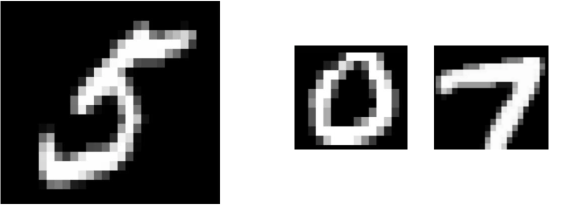
\includegraphics[scale=0.5, trim=0pt 0pt 0pt 0pt, clip]{motivation} 
  \caption{A motivational example where classification based on missing features would work in our dataset. Digit "5" from the MNIST dataset and its missing features named here: Feature 1 (on the left, circle-like feature) and Feature 2 (on the right, corner-line feature).}
  \label{fig:sample-motivation}
\end{figure}

In Fig.~\ref{fig:sample-motivation} we can see an example. Consider the given image of digit~5 (on the left) and two illustrative, very high-level features from our network model. Digit~5 can be defined in many ways, one of which is as "a digit missing these two features" (features are smaller squares on the right). To clarify, features are kernels (filters) from the convolutional layers in our model. Circle-like Feature 1 given here is present in digits 0, 6, 8, 9 while a sharp corner-line Feature 2 is present in digits 1, 2, 3 (e.g. top-right corner, or the middle part), 4, and 7. Digit 5 does not have these features, therefore we can check the input image and see if these features are missing. If they are, we can safely assume that we are looking at digit 5. This is not the only example where this is possible and this example is only given to clarify our way of thinking about "missing feature classification". 

In the following section section we discuss the motivation for developing more robust models not only for image processing but for various fields in deep learning applicable research.

\section{Robustness of Image Classifiers}

For a wide-spread adoption of systems that rely on neural networks it is needed to improve the current standard ways for training so the networks can be better prepared for intentional attacks and uncertain situations. It is very easy to describe this problem on the now standard task where neural networks are used -- image classification \cite{krizhevsky2012imagenet}. Neural networks are widely used for image classification, especially ones with convolutional layers. However, new research is taking place to investigate how these networks can handle real-world situations where there is noise in the image, the image is of low quality or where image is not given in full \cite{carlini2017towards, bastani2016measuring}. 

\subsection{Partial Input Classification}

Classification based on missing features, as presented here, is a new area of research in the neural network research field. We believe this new family of neural network models can be used in many different scenarios. The main benefit of these models described here is increasing robustness in partial input classification which is related to the neural network robustness, a growing topic in neural network research \cite{carlini2017towards}.

Our approach of classification based on missing features, as we will show, certainly can improve image classification accuracy with convolutional neural networks when they are faced with a task to classify an image by only seeing one part of it (partial input samples).

One example which is to benefit from this approach is when working with traffic signs. In self-driving cars -- a critical system that uses neural networks \cite{bojarski2016end}, traffic signs are processed as inputs from many cameras on a vehicle. These cameras are not perfect, but they produce very high quality images and usually the model used can easily detect and classify all traffic signs present in any given image. But what happens when a traffic sign is obstructed by another object, for example a tree or another car? A person in a similar situation can deduce what sort of a sign it is just by looking at one part of it and it is reasonable to require from the CNN models to be able to do the same. 

\chapter{Implementation}

In this chapter implementation of the classification based on missing features is explained. It is shown that for the image classification problem it is not only possible to train the models using only missing (negative) features, but also that these models show an increase in robustness when compared to traditional models of the same architecture.

In our experiment we decided to use widely known MNIST \cite{lecun1998mnist} dataset of handwritten digits. In addition to MNIST we also validated our work with the Extended MNIST dataset also known as EMNIST \cite{cohen2017emnist}.

MNIST dataset consists of 60000 training examples (pairs of images and labels) and 10000 testing or validation examples. To try and mimic a real life scenario where we wanted to test out our neural network model, we decided to make a few other validation sets which also contain 10000 examples. The way we did it is that we took the testing examples and removed some parts of every image, while keeping the label intact. It is important to clarify that we did not modify the training dataset. It is crucial to be able to train the network on the complete images, because in a real-world scenario we are unlikely to have partial inputs available for training. Also, we wanted to check if our network modification affects the standard, unmodified inputs.

\section{PMNIST dataset}

We did not want to limit ourselves to only one validation set because it is difficult to decide what data should be removed from the images. So we created multiple validation sets:

\begin{itemize}
  \item Horizontal cut dataset (top half removed) 
  \item Vertical cut dataset (left half removed)
  \item Diagonal cut dataset (two diagonal quarters of the image removed -- top-right and bottom-left)
  \item Triple cut dataset (three \(9x9\) pixel squares removed from coordinates (5, 5), (17,10), and (7,16) -- this is roughly 30\% of the input image removed, but the locations were chosen so that they cover vital parts of the digits (occlusion simulation)
\end{itemize}

\begin{figure}[!ht]
  \centering
  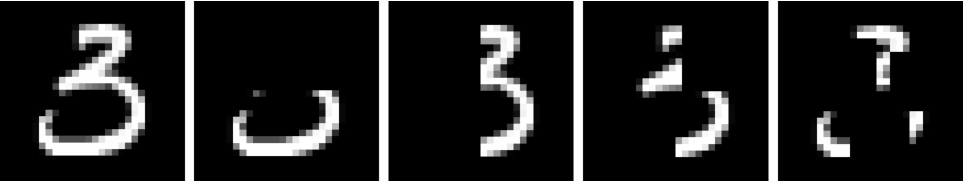
\includegraphics[scale=0.5, trim=0pt 0pt 0pt 0pt, clip]{datasetimages} 
  \caption{Example of digit 3 in our validation set; From left to right: unmodified -- original version, horizontally cut image -- top half removed, vertically cut image -- left half removed, diagonally cut image -- first and third quadrants removed, "triple cut" image -- three squares removed as described before}
  \label{fig:dsexamples}
\end{figure}

We will refer to this dataset as PMNIST or partial MNIST dataset. The final created dataset then consisted of:

\begin{itemize}
  \item 60000 training examples (unmodified)
  \item 10000 test examples (unmodified) 
  \item 10000 horizontally cut validation examples  
  \item 10000 vertically cut validation examples 
  \item 10000 diagonally cut validation examples
  \item 10000 "triple-cut" validation examples 
\end{itemize}

For the EMNIST dataset, we did exactly the same for two of its subsets. We first used the EMNIST-MNIST dataset whose structure is similar to MNIST dataset to validate our results, and then we tried our networks on the EMNIST-Balanced dataset which contains 131600 characters of digits and letters with 47 different classes for classification. 

The EMNIST-MNIST dataset, contains 60000 images and labels in the training set and 10000 images and labels in the test set -- exactly the same number of samples as in MNIST dataset. We used the process described above to generate four new validation sets, same as with PMNIST dataset. As for the EMNIST-Balanced dataset the same 85/15\% training and testing split was used to get a training set of 112800 images and labels and a test set of 18800 images and labels. Then, we generated four new test sets of size 18800, with different partial inputs for validation, same as before.

As both EMNIST and MNIST datasets have images of the same size (28x28 pixels) we used the exact same model architecture except for the last layer in the neural network which had to be changed to accommodate different number of classes in different datasets. The model is described in great detail in the following section.

It is important to note that during training the test sets and the newly introduced validation sets are not used. We want to completely avoid "peeking" at our validation data. That is why we split our dataset into three subsets: for training, testing and validation. All the models are trained and tested on complete input and output images and then validated on all validation data sets.

Another important remark is that approach described in this manuscript can work on any dataset, not just digits, letters etc. We chose these datasets because we can very clearly describe the features and their presence in a sample. With other datasets which have color or larger images this approach would still work but the features would be more difficult to interpret.

\section{Used Model architecture}

For the purpose of testing our theory a fairly standard model was used. The model is a default example model used in machine learning frameworks (e.g. PyTorch \cite{paszke2017pytorch}), so it was a good starting point for us to experiment with.

The model consists of five layers ordered in a common way -- a number of convolutional layers followed by a number of fully connected layers:

\begin{enumerate}
  \item Input layer -- 2D grayscale image of size \(28x28\) pixels
  \item 2D Convolutional layer 1 -- 20 kernels of size \(5x5\), with max-pooling of stride 2, and ReLU activation function 
  \item 2D Convolutional layer 2 -- 50 kernels of size \(5x5\), with max-pooling of stride 2, and ReLU activation function
  \item Fully-connected layer 1 -- 500 neurons, ReLU activation function
  \item Fully-connected layer 2 -- 10 output neurons for MNIST and EMNIST-MNIST cases, 47 output neurons for EMNIST-Balanced case, Softmax activation function
\end{enumerate}

We used SGD (Stochastic Gradient Descent) with learning rate of 0.01, and momentum of 0.5. These values were also not changed from the given model. Again, the given model was not modified in any way apart from introducing the conditional negation of the output vector of the last convolutional layer, as described in the following section. A performant model can used, and we will demonstrate how it performs with our modifications later in the dissertation. More on the model choice can be found in Section \ref{modelchoice}.

% dodati referencu na resnet u sinergiji

\section{The Negative Function}

In the introductory section we showed an example where it is easy to see how missing features can be used to classify a digit. While this example shows what we want to do it requires some additional knowledge about the data used. We want to use standard datasets without any additional knowledge so our approach can be used in any scenario. The main question was how can we obtain the missing features in the input sample. In this and the following sections we will explain how we can use existing knowledge from convolutional layers obtained with normal training in our modified approach. 

\subsection{Missing vs. negative features}

We also realize that the features in these features vectors are not binary. For a person it is very easy to decide whether a feature is either present or not present in an image. Neural networks are more flexible and can also say "how much" a feature is in a given sample. If the features were binary it would be trivial to find all the missing features in an image by replacing values in the feature vector with their opposites. Also, at this stage, it is very hard for us to say which missing features are more important than others, we simply try to classify based on all missing features. The term missing features is also not fully correct therefore, since it is very rare for a feature to be completely missing from the input image. That is why we use the term "negative feature" or "low-importance feature" interchangeably with the term "missing feature" throughout this thesis to emphasize this property of the features represented in an image.

\subsection{Activation Function Experiments}

For our approach of classification on missing features the model had to be modified slightly. We modified the forward pass in the network to negate the vector which represents what features are present in an image. When negated, this vector will represent what features are not present in an image. To demonstrate on an example, imagine a feature vector where 1 denotes a present feature and 0 denotes a missing feature. By simply replacing zeros with ones and vice-versa we can obtain a vector with all the missing features in the feature vector.

The negation process takes place between the exit of the last convolutional layer in a network and the entry to the first fully connected layer. It can be applied after the activation function application in the last convolutional layer, or by modifying the activation function as we will cover later. At that point the signal passed through the neurons is simply a feature vector describing what features were detected by convolutional layers. 

The negation operation largely depends on the activation function of the last convolutional layer. We have to negate the vector in a way that it represents the complete opposite of what would be the output of an unmodified network. The term "negate" probably can be replaced with "invert" in cases of some activation functions. 

For example, for hyperbolic tangent function (\(tanh\)) which is used as an activation function in neural networks a simple negation is enough. The \(tanh\) function always returns a value between \(-1\) and \(1\). If we agree that a present feature is represented by a value close to \(1\) and an absent feature is represented by a value of close to \(-1\), it is easy to see that negating a whole vector of \(tanh\) outputs would provide us a vector of features that are missing.

Rectified linear unit (\(ReLU\)) \cite{maas2013rectifier} functions are also widely used in neural networks. The \(ReLU\) function is different than the \(tanh\) function in that it returns values between zero and positive infinity. Here, simply negating the vector would not work, but calculating a new vector is not complicated. The output with a positive value represents a present feature and the value of zero represents a missing feature. If we apply a simple function as such:
%
\[
    f(x) = 1 - x
\]
%
we will get a vector representing what features are missing from the input image. 

In our model there were a total of 800 values (a vector of length 800) which is the output of the last convolutional layer and the input to the first fully connected layer. This vector represents all the present features and their positions in the input sample. As we are using (\(ReLU\)) activation function, we can negate the vector using the formula above.

\subsection{Influence of the Negative Function in forward and backward passes}

The implementation of the mentioned modification is very simple in PyTorch library. We only need to modify the "forward" function of the neural net Python module to negate the vector at a specific stage. The backwards pass is calculated automatically with autograd \cite{paszke2017automatic}.

\subsection{Negative feature selection process}

At this point we explained how and why the features are negated. We also mention that the features are not binary i.e. ones and zeros for present and missing features but rather a real valued numbers. That is why we used the already mentioned term of negative feature rather than missing feature. There is another issue with this approach worth considering. In the process of negating the features we assume that some features are positive or present. That features are then negated while the other features are marked as important (high activation values). This approach can be problematic as we mark all the low-activation features as important. Some of these features may as well be irrelevant to the specific class example for which we are training. It would be much better to know in advance which features are viable for negation per-class so not all low-importance features are activated. This activation can be seen as noise with which our models can work, as demonstrated, but it certainly help to select features for negation beforehand.  

\subsubsection{Detecting relevant features per-class for negation}

In this section, we propose an idea for a solution for finding relevant features per class. These selected features can be used for negation while the other irrelevant features are not modified. Similarly to convolutional activation atlases we want to find what features are activated (their activation value is above a certain threshold) for specific classes of images during training. With our modified training process this can be achieved in the following way. 

When the "pre-training" step of the process where the normal network is trained and convolutional layers are obtained we can use this model before discarding parts of it to extract what features (here output of the convolutional block) are important per class. The number of features is finite and they are used as a one dimensional tensor which is then passed as input to the fully-connected layers. For each class we remember all the activations indices which we obtain with forward passes through the network. Then, these indices are remembered and used for negation during training. It is important to say that these indices can only be used during training and not during testing. This is because to select certain features we have to know the correct class which is not available during testing. This is an issue which has to be considered in the future, because we want the model to behave the same in the training and testing phases. We will revisit this idea in the future work and validate our assumptions.

\section{Training process}

In this section training processes related to the negative learning method are described with the focus on two very important processes: multiple phase training and convolutional kernel freezing. To successfully implement the classification based on missing features model our experiments have shown that both of these techniques have to be used.

\subsection{Multi-phase training}

The training processes are also modified from the standard process. The unmodified network is trained for 10 epochs in the provided model. After that, no significant increase in accuracy is noted, as the network already gets around 99\% accuracy on the test set.

During the Negative Deep Learning model/hypothesis testing one interesting concept was used -- multi-phase training. Multiple phase training is a training process where after a number of training epochs some layers are frozen and reused and some of the layers are reset. In a way, multiple phase training is a regularization technique similar to Dropout with \(P = 1.0\) where some layers are completely destroyed and retrained during training. 

In our concrete example multiple phase training was used to extract and reuse convolutional layers from an image classification model. After a number of epochs all the convolutional kernels were extracted and used in other (negative) models.

\subsubsection{ONN Model}

The first training process tested is to simply apply the model upgrade we described in the previous chapter and train the network normally. We called this model "ONN" (only negate network). Although this approach gives us some improvements, it does not represent fully what we wanted to do. Because the network is modified to negate the vector representing the features in the input image, we observed that our new model adapted to our layer inversion modification. The change affected the backwards pass in the network so the convolutional filters in convolutional layers were completely different opposed to the standard network. In other words, the features found in input images were not the same -- the network learned them in a different way. As we wanted the features to remain the same and only to modify the later stages of the network, we thought of the second training process which allows this. Our goal is to classify on the same features but to emphasize those which are missing.

\subsubsection{Hybrid training mode (first actual negative model)}

The second process requires a few extra steps and is as follows. The training process begins for a number of epochs where the "negation layer" is inactive. This is so that the convolutional layers inside the network learn all the features in the training data. In this step the filters inside the convolutional layers will learn both the high-level and low-level features of digits given the digit images from the dataset. We do this training step for 10 epochs, which is enough for the model to learn the features well enough.

The next step consists of freezing the convolutional layers and resetting the fully connected layers. The freezing of convolutional layers is necessary so that the further training does not affect them. The features represented in the convolutional kernels are learned already and we do not wish to modify them. The convolutional layers are simply going to be used for feature extraction at this and future points. 

Resetting the fully connected layers is also necessary as we want the network to start over the learning process but to classify based on the missing features in an image. Resetting the layers simply means re-initializing them with the same initializer used in the model setup.

With the features learned, convolutional layers frozen and fully connected layers ready for new training, we can activate the modification in the model which will negate or invert the output of the convolutional layer. This is made possible by dynamic nature of execution which is available in PyTorch neural network library. This is the main reason why it was chosen to be used for this work. 

The training is then continued on for another 10 epochs, making it 20 epochs in total which is more than normal training. It is important to clarify that while our modified network is in total trained for 10 epochs more than the standard network its fully connected layers are reset after the tenth epoch making it so the final models are equal in quantity of training received. Convolutional layers only receive the 10 epochs of training also, before being frozen. This approach is a hybrid between normal and our new way of training so we called it "HN" ("hybrid network").

\subsubsection{More on Convolutional Kernel Freezing}

For most of here mentioned models we use freezing of convolutional kernels. Freezing is a process of setting convolutional layers as fixed, constant values after they have been learned. The freezing of the convolutional layers is important from the analysis standpoint as we want to test our model modifications which are currently after the convolutional blocks. If we were not to freeze the convolutional layers, they would change their parameters during training -- and this is not desired behaviour. 

Freezing of the layers is a procedural process where one has to iterate through convolutional filter parameters (conv. kernels) and mark them as constant. In the PyTorch framework this is done with the "requires\_grad" field.

Freezing of the convolutional layers (or other parts of a neural network models) is a common technique when using pre-trained models. The idea behind pre-trained models is simple: a model trained on a dataset (usually large, not easy to retrain) is extended with few layers on top to be used for some different task. One example where this approach is popular is with image classification. There, it is common to use very deep and complex models trained on the ImageNet Dataset as frozen feature extractors. In addition, a simple fully-connected neural network is added "on-top" of the ImageNet model and trained to classify custom image datasets.

\subsubsection{Modified Hybrid Training Processes}
\label{altmodel}

We also experimented with some modifications to the hybrid training process.

The first modification to our described process is to skip resetting the fully connected layers after the features were learned (referred in the results tables as "NR" -- "no reset").  In a way, this means that the network continues training after this step but in a different way. The reasoning for this approach is that there may still be useful weights in our fully connected layer which can improve the model accuracy even after we have trained with our inversion modification in place. We wanted to try to combine standard training with our modified way to see if synergy between standard and our training process has any effect.

Another modification we tried is to alternate between normal training and training with inversion modification. For a number of epochs, we train the network so that one epoch the network is unmodified and another epoch is with the inversion modification in place. This is an extension of the previous modification because we wanted to make sure that the order of training is not important. This method we called "ALT" method as it alternates between ways of training. We also noticed that the "ALT" training model works best with smaller learning rates. When using large learning rates, the model would change the weights too much when switching from one way of propagation to another. This is something to be aware of, if using this approach.

\subsubsection{Note on training process}

For all processes and models, because random initialization is used we made sure to test several times to avoid any coincidental results. In development stages a constant random seed method was used for reproducible results. The libraries used for development have all been set to use determinism wherever possible.

\chapter{Testing}

In this chapter we describe the testing processes where we validate our models and we present the results.

\section{Results on the MNIST and PMNIST datasets}

Since we are introducing a new neural network model in this work, we decided that the best baseline in comparing the results would be a traditional neural network with the same architecture ("SN"). This way we can be sure that our modification in the model is what we are benchmarking.

\subsection{Note about model choice} \label{modelchoice}

We are aware that a model architecture which would give even better results compared to our own model probably exists. It is a very difficult task in finding such a model, while making sure that our modification actually does affect the accuracy increase. This is why we decided to test our approach on a very well-known model to see how it behaves. Since our modification is simple and can be applied to any CNN model, we will definitely experiment with other models (network architectures) on our newly introduced validation sets to see how they perform.

After testing the models on the mentioned datasets we obtained the following results. First, we present the results on unmodified testing sets.

\begin{table}[ht]
  \centering
  % note the S[] column specification provided by the siunitx package
  \begin{tabular}{rS[table-format=2.1]S[table-format=2.1]S[table-format=2.1]S[table-format=2.1]S[table-format=2.1]S[table-format=2.1]}
    \toprule
     \textit{Dataset/Model} & SN & ONN & HN & NR & ALT \\
    \midrule
    {Unmodified MNIST} & {99.13} & {98.90} & {99.18} & {99.21} & {99.05} \\
    {Unmodified EMNIST-MNIST} & {99.18} & {99.07} & {99.16} & {99.15} & {99.00} \\
    {Unmodified EMNIST-Balanced} & {87.14} & {87.62} & {87.38} & {86.78} & {87.92} \\
    
    \bottomrule
  \end{tabular}
  %
  \caption{Results with accuracy for all models and unmodified testing datasets. Here, SN denotes the standard, unmodified network, ONN denotes the network only trained with layer negation and HN denotes Hybrid network which was trained normally for a number of epochs but was then switched to negate the output of the last convolutional layer. The NR and ALT models are trained as explained in previous section. NR model is the model which is not reset (NR) after the inversion modification and the ALT model is extension of the NR model where the normal and inversed training takes place in alternating (ALT) epochs. All the values are percents which depict validation accuracy of a network on a given dataset.}
  \label{tab:results-unmodified}
\end{table} 

As seen in Tab.~\ref{tab:results-unmodified} the modified network models performed better in almost all of the standard unmodified test sets showing that classification on missing features does slightly improve accuracy when the input sample is given in full. We want to emphasize that this method of training while longer and slower does not negatively affect the network performance when the input is given in full. This is something we were hoping for to be achieved. These results also show that our initial assumption was correct -- it is possible to train a neural network to classify based on missing features.

In Tab.~\ref{tab:results-pmnist}, \ref{tab:results-emnistmnist} and \ref{tab:results-emnist} we present the accuracy percentages on the newly introduced validation sets. In Tab.~\ref{tab:results-pmnist} we show the results on the four PMNIST validation sets while in Tab.~\ref{tab:results-emnistmnist} and \ref{tab:results-emnist} we present the result on the four validation sets generated for EMNIST-MNIST and EMNIST-Balanced datasets, respectively.

\begin{table}[ht]
  \centering
  % note the S[] column specification provided by the siunitx package
  \begin{tabular}{rS[table-format=2.1]S[table-format=2.1]S[table-format=2.1]S[table-format=2.1]S[table-format=2.1]S[table-format=2.1]}
    \toprule
     \textit{Dataset/Model} & SN & ONN & HN & NR & ALT \\
    \midrule
    {Horizontal cut} & {44.71} & {48.96} & {52.33} & {56.07} & {41.60} \\
    {Vertical cut} & {57.46} & {64.64} & {60.45} & {66.07} & {69.66} \\
    {Diagonal cut} & {52.97} & {59.59} & {55.40} & {56.01} & {62.49} \\
    {Triple cut} & {40.68} & {34.62} & {41.19} & {41.73} & {46.40} \\
    
    \bottomrule
  \end{tabular}
  %
  \caption{Results with accuracy for all models used on newly introduced PMNIST validation sets.}
  \label{tab:results-pmnist}
\end{table} 

\begin{table}[ht]
  \centering
  % note the S[] column specification provided by the siunitx package
  \begin{tabular}{rS[table-format=2.1]S[table-format=2.1]S[table-format=2.1]S[table-format=2.1]S[table-format=2.1]S[table-format=2.1]}
    \toprule
     \textit{Dataset/Model} & SN & ONN & HN & NR & ALT \\
    \midrule
    {Horizontal cut} & {49.07} & {51.34} & {54.76} & {48.70} & {48.73} \\
    {Vertical cut} & {31.10} & {28.10} & {32.91} & {28.62} & {31.12} \\
    {Diagonal cut} & {58.43} & {61.22} & {59.37} & {58.18} & {61.50} \\
    {Triple cut} & {46.78} & {49.63} & {53.90} & {48.99} & {47.44} \\
    
    \bottomrule
  \end{tabular}
  %
  \caption{Results with accuracy for all models used on newly introduced EMNIST-MNIST validation sets.}
  \label{tab:results-emnistmnist}
\end{table} 

\begin{table}[ht]
  \centering
  % note the S[] column specification provided by the siunitx package
  \begin{tabular}{rS[table-format=2.1]S[table-format=2.1]S[table-format=2.1]S[table-format=2.1]S[table-format=2.1]S[table-format=2.1]}
    \toprule
     \textit{Dataset/Model} & SN & ONN & HN & NR & ALT \\
    \midrule
    {Horizontal cut} & {20.95} & {26.97} & {26.34} & {19.32} & {26.53} \\
    {Vertical cut} & {22.23} & {20.02} & {22.19} & {19.50} & {24.36} \\
    {Diagonal cut} & {27.91} & {30.14} & {30.79} & {25.80} & {26.83} \\
    {Triple cut} & {20.39} & {22.88} & {21.07} & {21.81} & {19.83} \\
    
    \bottomrule
  \end{tabular}
  %
  \caption{Results with accuracy for all models used on newly introduced EMNIST-Balanced validation sets.}
  \label{tab:results-emnist}
\end{table} 

\begin{table}[ht]
  \centering
  % note the S[] column specification provided by the siunitx package
  \begin{tabular}{rS[table-format=12.1]S[table-format=32.1]S[table-format=42.1]}
    \toprule
     \textit{Dataset} & {Best model} & {Accuracy} & {Delta} \\
    \midrule
    {Unmodified - PMNIST}  & {NR} & {99.21} & {0.08} \\
    {Horizontal cut - PMNIST} & {NR} & {56.07} & {11.36} \\
    {Vertical cut - PMNIST} & {ALT} & {69.66} & {12.20} \\
    {Diagonal cut - PMNIST} & {ALT} & {62.49} & {9.52} \\
    {Triple cut - PMNIST} & {ALT} & {46.40} & {5.72} \\
    {Unmodified - EMNIST-MNIST} & {HN} & {99.16} & {-0.02} \\
    {Horizontal cut - EMNIST-MNIST} & {HN} & {54.76} & {5.69} \\
    {Vertical cut - EMNIST-MNIST} & {HN} & {32.91} & {1.81} \\
    {Diagonal cut - EMNIST-MNIST} & {ALT} & {61.50} & {3.07} \\
    {Triple cut - EMNIST-MNIST} & {HN} & {53.90} & {7.12} \\
    {Unmodified - EMNIST-Balanced} & {ALT} & {87.92} & {0.78} \\
    {Horizontal cut - EMNIST-Balanced} & {ONN} & {26.97} & {6.02} \\
    {Vertical cut - EMNIST-Balanced} & {ALT} & {24.36} & {2.13} \\
    {Diagonal cut - EMNIST-Balanced} & {HN} & {30.79} & {2.88} \\
    {Triple cut - EMNIST-Balanced} & {ONN} & {22.88} & {2.49} \\
    
    \bottomrule
  \end{tabular}
  %
  \caption{Results with showing what models worked best with different test and validation sets. The "Accuracy" column shows final, highest accuracy achieved while the "Delta" column shows accuracy gain over the standard unmodified network. Both "Accuracy" and "Delta" columns are given in percentages.}
  \label{tab:results-final}
\end{table}

When comparing our training processes or models (Tab.~\ref{tab:results-final}), it is clear to see that some of them perform better in certain scenarios. However, apart from the 0.02\% accuracy loss on the unmodified EMNIST-MNIST test set, it is uniform that the newly introduced models featuring some shape of classification based on missing features outperform traditional neural network models, and in some cases by large margins. This is the most important finding in this experiment with our new models.

We also notice that models which use convolutional layer freezing outperform the model which just negates the convolutional feature vector (ONN). Also, strong performance of ALT network suggests there is some benefit of combining traditional neural network models with our newly introduced ones. As for choosing what model would work best in a certain scenario, it is difficult to say with certainty. We suggest trying different models and deciding by testing them. 

The different datasets we used all behave similarly. We see the largest accuracy increase of 12.2\% with the vertical cut validation set in the PMNIST set.

\subsection{Summary of the first experiments}

Here we present concisely the summary of experiments with the classification based on missing features:

\begin{itemize}
  \item It is possible to train a convolutional neural network to classify based on missing features in the input sample.
  \item Our approach of "negating" feature vectors before passing them to fully connected layers implements this idea and shows that this simple modification can help in a scenario where a partial input is given.
  \item The performance of convolutional neural networks, as expected, degrades greatly when we use partial inputs. 
  \item The PMNIST dataset and other partial datasets based on EMNIST dataset, can be used for checking how a network behaves when given a partial input to classify.
  \item We also showed four similar but different training techniques to maximize the usefulness of our modification. These training techniques can be used to experiment with different datasets.
\end{itemize}

The results show that classification based on missing features is possible and that these new models we introduced help in partial input scenarios. Our approach, albeit much simpler than some other approaches (e.g. training with adversarial examples) can also help with a very difficult real-world problem of having partial inputs to classify in a critical environment. The partial input example is only one of many use cases for our models that we hope to discover.

\subsection{Influence of multiple-step training}
During the development of this model, as we mentioned before, a multiple-step training process was used. In this process some layers were frozen and some layers were reset which led to the network having hot starting training properties. similarly to fine-tuning of the model. In other words the network did not learn the patterns from scratch but rather had a baseline in the form of trained convolutional layers. It is therefore important to see how this process contributed to our overall result and to validate that it is the change in our negative feature approach that brings the performance increase and not the fine tuning of the network with the multiple-step training process. 

To do so we created a simple experiment where a normal network without the negative path activated is trained for a number of epochs and then similarly to our negative network we freeze the convolutional layers, reset the fully connected layers and continue training. The process therefore is exactly the same as for training the hybrid model but without the negative activation function.

In the Table \ref{tab:results-twophase} the results are shown where the two-phase approach did not bring the same level of improvement as our negative model approach. In some cases the performance is severely degraded as can be seen in the table. This experiment confirms our intuition about the negative model and proves that a simple modification of the training process where multiple phases are added does not bring increased performance.

\begin{table}[ht]
  \centering
  \begin{tabular}{rS[table-format=2.1]S[table-format=2.1]S[table-format=2.1]S[table-format=2.1]S[table-format=2.1]S[table-format=2.1]S[table-format=2.1]}
    \toprule
     \textit{Dataset/Model} & SN & ONN & HN & NR & ALT & TP \\
    \midrule
    {Unmodified MNIST} & {99.13} & {98.90} & {99.18} & {99.21} & {99.05} & {96.79} \\
    {Horizontal cut} & {44.71} & {48.96} & {52.33} & {56.07} & {41.60} & {24.84} \\
    {Vertical cut} & {57.46} & {64.64} & {60.45} & {66.07} & {69.66} & {43.82} \\
    {Diagonal cut} & {52.97} & {59.59} & {55.40} & {56.01} & {62.49} & {54.44} \\
    {Triple cut} & {40.68} & {34.62} & {41.19} & {41.73} & {46.40} & {47.37} \\
    
    \bottomrule
  \end{tabular}
  %
  \caption{Results with accuracy for all models used on newly introduced PMNIST validation sets. Included in this table as a validation effort is also the two-phase normal non-negative network (last column, TP for two-phase network).}
  \label{tab:results-twophase}
\end{table} 

\subsection{Negative Convolutional Kernel Experiments}

A valid question for our model definition is why not use negation on the convolutional kernel themselves, rather than to use them after the activation function is applied. While certainly possible, there is hardly any difference in trained models performance in our experiments. There are several advantages and disadvantages to this approach.

The greatest advantage is in that to use negative learning we only need to negate (apply \( new\_kernel\_weights = - old\_kernel\_weights \) and \( new\_kernel\_biases = -  old\_kernel\_biases \)) convolutional layers independently of our activation function choice. As we mentioned earlier the negation function needs to take into consideration what is the domain of value which are output from the last convolutional layer and its activation function. If we are negating the kernels directly we can do so without the additional knowledge (and implementation) about the activation function. 

From the implementation standpoint, another benefit is that we do not have branches in our network forward pass as we had before. This allows us to use static computational graphs (e.g. TensorFlow implementation) instead of dynamic graphs (PyTorch) which can lead to increase in training and inference speed.

There are also however several disadvantages. 

First of all, the kernels must be learned before they are negated eliminating several of our newly implemented models. The pure negative (non-hybrid) model cannot be trained consistently with other models in this way since we do not know the kernels and their negation. In other works we need to use negation also during the training of the kernel themselves, which in this scenario is not possible. Another is the alternating hybrid model. As we cannot use branches in our forward (and backward) pass to shift the weight changes from the gradient descent, we cannot train this model. We could perhaps keep a copy of the kernel weights and biases and somehow compute the updates, but it would be very complicated and probably without any benefit to the performance.

We strongly believe that the dynamic, branched approach is better for its flexibility. We are fully in control of the negation process only in this case.

We present here the results for the MNIST and PMNIST datasets (experiments have been conducted for MNIST, PMNIST, EMNIST-Balanced and EMNIST-MNIST datasets, all have similar results to our other experiments, code is available) to show that negation of the kernels does not bring performance in comparison to our "branched" dynamic approach of negating the signal after the activation function of the last convolutional layer. This network is exactly the same architecture as all the other models we describe in this part, the only difference is that the negation of the features is removed from the forward pass definition function and the kernel are negated directly. The kernel negation process takes place after half of the total number of epochs of training (same as with the other models, where we activated the negative branch in the same time point). We present results for the hybrid and hybrid-nr models as they are only ones compatible. We also include the baseline model for easier reading. 

\begin{table}[ht]
  \centering
  % note the S[] column specification provided by the siunitx package
  \begin{tabular}{rS[table-format=2.1]S[table-format=2.1]S[table-format=2.1]S[table-format=2.1]S[table-format=2.1]S[table-format=2.1]}
    \toprule
     \textit{Dataset/Model} & SN & HN & NR  \\
    \midrule
    {Unmodified MNIST} & {99.01} & {98.74} & {98.62} \\
    {Horizontal cut} & {45.52} & {47.32} & {48.74} \\
    {Vertical cut} & {60.37} & {58.36} & {60.15}  \\
    {Diagonal cut} & {56.47} & {60.87} & {57.10} \\
    {Triple cut} & {41.83} & {41.56} & {46.57} \\
    
    \bottomrule
  \end{tabular}
  %
  \caption{Results with accuracy for all models using direct kernel negation, on MNIST/PMNIST validation sets.}
  \label{tab:results-kerneg}
\end{table} 

In Table \ref{tab:results-kerneg} we can see that we obtained very similar results to our other experiments, leading us to believe that it is up to the researcher to choose what implementation is better to use in which scenario taking into count the advantages and disadvantages of both methods we propose here.

\subsection{Other activation functions}

So far we have shown how to negate the ReLU function and how it is possible to use negative learning concepts when using this function. It is of course possible to use other activation functions as we will show in this subsection. For our tests we originally chose the ReLU activation function as it is today's most popular and performant choice in modern neural network architectures.

In this subsection we display results of our experiments with three additional activation functions: \( sigmoid \), \( tanh \) and \( ReLU6 \). \( Sigmoid \) activation function was one of the first non-linear activation function used for artificial neural networks. As it outputs values in the range from \( 0 \) to \( 1 \) our negation formula \( f(x) = 1 - x \) can be used without further modifications. For the \( tanh \) activation function the negation function had to be modified slightly as the \( tanh \) function outputs values in the range from \( -1 \) to \( 1 \). It is therefore necessary to use a different negation function: \( f(x) = -x \). Lastly for the \( ReLU6 \) activation function, a modification of the \( ReLU \) activation function with a hard ceiling at the value \( 6 \) we used \( f(x) = 6 - x \).

All the results displayed in the following tables show that it is possible to use negative learning concepts we mention here with different activation functions on the MNIST dataset with this model. As for performance, it is also clear that there are again benefits, especially in the case of partial inputs. It is important to note however that these results are not directly comparable with the results we showed for the \( ReLU \) model. Activation function choice is an important architecture change, therefore the models become incomparable. 

Presented results are for the MNIST/PMNIST dataset. Experiments have been performed also on the EMNIST-MNIST and EMNIST-Balanced datasets with similar findings. Full results are available in the source code repository of the thesis.

\begin{table}[ht]
  \centering
  % note the S[] column specification provided by the siunitx package
  \begin{tabular}{rS[table-format=2.1]S[table-format=2.1]S[table-format=2.1]S[table-format=2.1]S[table-format=2.1]S[table-format=2.1]}
    \toprule
     \textit{Dataset/Model} & SN & ONN & HN & NR & ALT \\
    \midrule
    {MNIST} & {93.07} & {93.39} & {94.42} & {94.39} & {91.03} \\
    {Horizontal cut} & {32.62} & {33.64} & {33.75} & {33.94} & {36.36} \\
    {Vertical cut} & {35.28} & {33.99} & {39.50} & {38.65} & {38.76} \\
    {Diagonal cut} & {54.44} & {54.68} & {55.49} & {57.94} & {49.79} \\
    {Triple cut} & {43.67} & {44.17} & {45.49} & {53.86} & {40.20} \\
    
    \bottomrule
  \end{tabular}
  %
  \caption{Results with accuracy for all models used on the PMNIST validation sets while using \( sigmoid \) activation function}
  \label{tab:results-sigmoid}
\end{table} 

\begin{table}[ht]
  \centering
  % note the S[] column specification provided by the siunitx package
  \begin{tabular}{rS[table-format=2.1]S[table-format=2.1]S[table-format=2.1]S[table-format=2.1]S[table-format=2.1]S[table-format=2.1]}
    \toprule
     \textit{Dataset/Model} & SN & ONN & HN & NR & ALT \\
    \midrule
    {MNIST} & {98.85} & {98.84} & {98.84} & {98.88} & {97.54} \\
    {Horizontal cut} & {41.58} & {38.46} & {41.98} & {40.21} & {45.34} \\
    {Vertical cut} & {43.91} & {43.68} & {48.84} & {52.35} & {47.30} \\
    {Diagonal cut} & {54.11} & {54.74} & {54.50} & {57.81} & {63.46} \\
    {Triple cut} & {40.52} & {38.31} & {42.78} & {43.66} & {47.46} \\
    
    \bottomrule
  \end{tabular}
  %
  \caption{Results with accuracy for all models used on the PMNIST validation sets while using \( tanh \) activation function}
  \label{tab:results-tanh}
\end{table} 

\begin{table}[ht]
  \centering
  % note the S[] column specification provided by the siunitx package
  \begin{tabular}{rS[table-format=2.1]S[table-format=2.1]S[table-format=2.1]S[table-format=2.1]S[table-format=2.1]S[table-format=2.1]}
    \toprule
     \textit{Dataset/Model} & SN & ONN & HN & NR & ALT \\
    \midrule
    {MNIST} & {99.02} & {10.32} & {98.94} & {97.61} & {9.58} \\
    {Horizontal cut} & {41.37} & {10.32} & {44.57} & {31.30} & {9.58} \\
    {Vertical cut} & {57.17} & {10.32} & {57.33} & {63.42} & {9.58} \\
    {Diagonal cut} & {55.68} & {10.32} & {62.15} & {59.87} & {9.58} \\
    {Triple cut} & {40.65} & {10.32} & {42.57} & {41.76} & {9.58} \\
    
    \bottomrule
  \end{tabular}
  %
  \caption{Results with accuracy for all models used on the PMNIST validation sets while using \( ReLU6 \) activation function}
  \label{tab:results-relu6}
\end{table} 

From the tables shown here we can see that in all cases there is at least one variation of a negative model outperforming the traditional model, proving our hypothesis.

For the \( ReLU6 \) experiments we can see that some models are unable to converge, the only negative model and the alternating model. We strongly believe that is because of our negation function. This outlier proved very important as we understood our negation function more accurately. It is very important to negate the ReLU (and possibly other activation functions) in a way that there are negative values (for negative features) in the new output vector. These values when propagated further through the network will be annulled naturally through other ReLU activations. We assume this is important for our model, to learn what features need to ignored in a way. To validate this assumption, we made a similar experiment using a different negation function for the \( ReLU6 \) activation function:  \( f(x) = 3 - x \). This will allow the strongly positive, present features to have values less than 0 in the output vector.

\begin{table}[ht]
  \centering
  % note the S[] column specification provided by the siunitx package
  \begin{tabular}{rS[table-format=2.1]S[table-format=2.1]S[table-format=2.1]S[table-format=2.1]S[table-format=2.1]S[table-format=2.1]}
    \toprule
     \textit{Dataset/Model} & SN & ONN & HN & NR & ALT \\
    \midrule
    {MNIST} & {99.02} & {98.92} & {99.04} & {99.14} & {99.04} \\
    {Horizontal cut} & {41.37} & {45.75} & {44.28} & {45.52} & {52.69} \\
    {Vertical cut} & {57.17} & {58.70} & {55.61} & {65.31} & {61.85} \\
    {Diagonal cut} & {55.68} & {62.23} & {59.24} & {58.53} & {60.77} \\
    {Triple cut} & {40.65} & {42.26} & {39.82} & {44.91} & {43.63} \\
    
    \bottomrule
  \end{tabular}
  %
  \caption{Results with accuracy for all models used on the PMNIST validation sets while using \( ReLU6 \) activation function and the \( f(x) = 3 - x \) negation function.}
  \label{tab:results-relu6new}
\end{table} 

As can be seen in the table, the results suggest that our hypothesis is correct, some form of less than zero values when using rectified linear units (ReLU) is needed. This idea will be examined in more detail in the future research.

Another example where this can be seen is if \( LeakyReLU \) activation function is used. \( LeakyReLU \) function is very similar to \( ReLU \) function but it allows some of the negative values to "leak through" whereas \( ReLU \) cuts off all negative values. \( LeakyReLU \) can be defined as \( LeakyReLU(x) = max(0,x) + negative\_slope * min(0,x) \) where \( negative\_slope \) is a variable factor which dictates how much leaking of the close-to-zero values is allowed. With this activation function it is extremely important to allow for some negative values to pass through as we mentioned before for the \( ReLU6 \) activation function. This function is also tested and can be used for negative learning with the same negation as \( ReLU \), the results for MNIST/PMNIST validation are in the following table.

\begin{table}[ht]
  \centering
  % note the S[] column specification provided by the siunitx package
  \begin{tabular}{rS[table-format=2.1]S[table-format=2.1]S[table-format=2.1]S[table-format=2.1]S[table-format=2.1]S[table-format=2.1]}
    \toprule
     \textit{Dataset/Model} & SN & ONN & HN & NR & ALT \\
    \midrule
    {MNIST} & {98.96} & {98.97} & {99.12} & {99.21} & {99.06} \\
    {Horizontal cut} & {42.57} & {53.36} & {49.05} & {51.53} & {47.96} \\
    {Vertical cut} & {60.32} & {65.43} & {61.17} & {69.80} & {63.84} \\
    {Diagonal cut} & {54.16} & {61.20} & {59.97} & {57.98} & {60.69} \\
    {Triple cut} & {41.19} & {40.07} & {38.89} & {42.52} & {43.76} \\
    
    \bottomrule
  \end{tabular}
  %
  \caption{Results with accuracy for all models used on the PMNIST validation sets while using \( LeakyReLU \) activation function (\( negative\_slope = 0.1\)) and the \( f(x) = 1 - x \) negation function.}
  \label{tab:results-leakyrelu}
\end{table} 

\subsection{Corner occlusions}

In addition to our previous experiments with removing parts of the image we decided to experiment with one more special case of image occlusion -- corner occlusion. This type of occlusion is very common in modern images and it simply means that one triangular part of the image (in our case bottom left corner) is removed, or behind another object. An example on the CIFAR-10 dataset can be seen in Figure \ref{fig:cbomf3}.

\begin{figure}
    \centering
    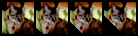
\includegraphics[width=0.7\textwidth]{figures/fig3.png}
\caption{Input example \#8 from CIFAR-10 validation set with various levels of occlusion added. From left to right: original image, \( 10\% \) removed, \( 20\% \) removed, \( 30\% \) removed}
\label{fig:cbomf3} 
\end{figure}

We carried out all the experiments as before but with these new validation datasets. The experiments were done with varying number of pixels removed from 10\% of the image to 50\% of the image. The results can be seen in the following table.

\begin{table}[ht]
  \centering
  % note the S[] column specification provided by the siunitx package
  \begin{tabular}{rS[table-format=2.1]S[table-format=2.1]S[table-format=2.1]S[table-format=2.1]S[table-format=2.1]S[table-format=2.1]}
    \toprule
     \textit{Dataset/Model} & SN & ONN & HN & NR & ALT \\
    \midrule
    {Occlusion, 10\%} & {98.97} & {98.97} & {99.09} & \textbf{{99.19}} & {99.09} \\
    {Occlusion, 20\%} & {98.97} & {98.98} & {99.09} & \textbf{{99.17}} & {99.09} \\
    {Occlusion, 30\%} & {98.62} & {98.53} & {98.89} & \textbf{{98.90}} & {98.81} \\
    {Occlusion, 40\%} & {79.27} & {77.88} & {79.69} & \textbf{{81.01}} & {80.26} \\
    {Occlusion, 50\%} & {36.55} & {45.53} & {41.76} & \textbf{{49.35}} & {43.64} \\
    
    \bottomrule
  \end{tabular}
  %
  \caption{Results with accuracy for all models used on the new corner occlusion validation sets. Bold are the best models per dataset. Hybrid no-reset network performs best here.}
  \label{tab:results-corner}
\end{table} 

We can see that the accuracy slowly decreases as we remove more image data, as expected. We can also confirm that our models are more robust in comparison with the normal baseline neural network in all the cases of corner occlusion, in some cases (e.g. 50\% occlusion) even by as much as 12.8 \%, a great result. We can also see that the MNIST dataset has high quality as all images are centered and roughly the same size. Even with 30\% of the corner data removed most of the relevant data remains in the image.

Test have been performed on other datasets we mention here (EMNIST-MNIST, EMNIST), with similar results. Full results can be found in the code repository.

Other occlusion variants (e.g. top-right or other corners) remain to be tested. 

\section{Robustness to Adversarial Attacks}
\label{sec:adversarial}

A topic which should be mentioned here is adversarial attacks on neural networks research \cite{bastani2016measuring}. 

There have been some research papers similarly exploring how to increase robustness of neural networks when the inputs have been tampered with. However, our approach is not directly comparable with their approaches for many reasons i.e. different network architectures, usage of partial inputs in training, usage of adversarial examples in training, etc.

In \cite{globerson2006nightmare} the MNIST \cite{lecun1998mnist} dataset used in our work was also used to investigate robustness of neural networks. In our paper parts of the input image were removed as will be explained later, while the authors in \cite{globerson2006nightmare} describe a way to combine two images as an adversarial example input.

\cite{szegedy2013intriguing} and \cite{goodfellowexplaining} described also on the MNIST dataset different modifications to the input image which affect the model greatly. In \cite{szegedy2013intriguing} MNIST dataset was used to investigate how different elements in input images maximize some network activations. The second part of the paper describes an adversarial attack on the network using previously gathered information. Our paper differs from this paper in that we are investigating how missing features are affecting classification instead of what features affect it the most, and that we are also using a convolutional neural network, while in this paper a traditional multi-layer fully connected network is used. Also in the mentioned paper, authors suggest that training with a mixture of adversarial and clean examples is a way to achieve better performance. In our case, we did not want to train on our generated adversarial (partial) examples, as will be explained later. Similarly in \cite{goodfellowexplaining} adversarial examples are being used to increase neural network robustness, but they are being used during training. 

\subsection{White-box attacks (Fast Gradient Sign Method attack on the negative models)}

To evaluate our model robustness with regard to adversarial attack we first experimented with the most-popular white-box method: Fast Gradient Sign Method (FGSM). \cite{goodfellowexplaining} This white-box attack uses gradient information from the forward pass of the model in combination with gradient ascent to maximize the loss function we normally use for training. This method step is very similar to training the model apart from that the model is in evaluation mode (locked weights) and gradient ascent is used to modify the input image. That modified input image becomes an adversarial example. The adversarial image is often indistinguishable (to humans) from the original image but wrongly classified by the model. One example can be seen in the Figure. 

\begin{figure}
\centering
  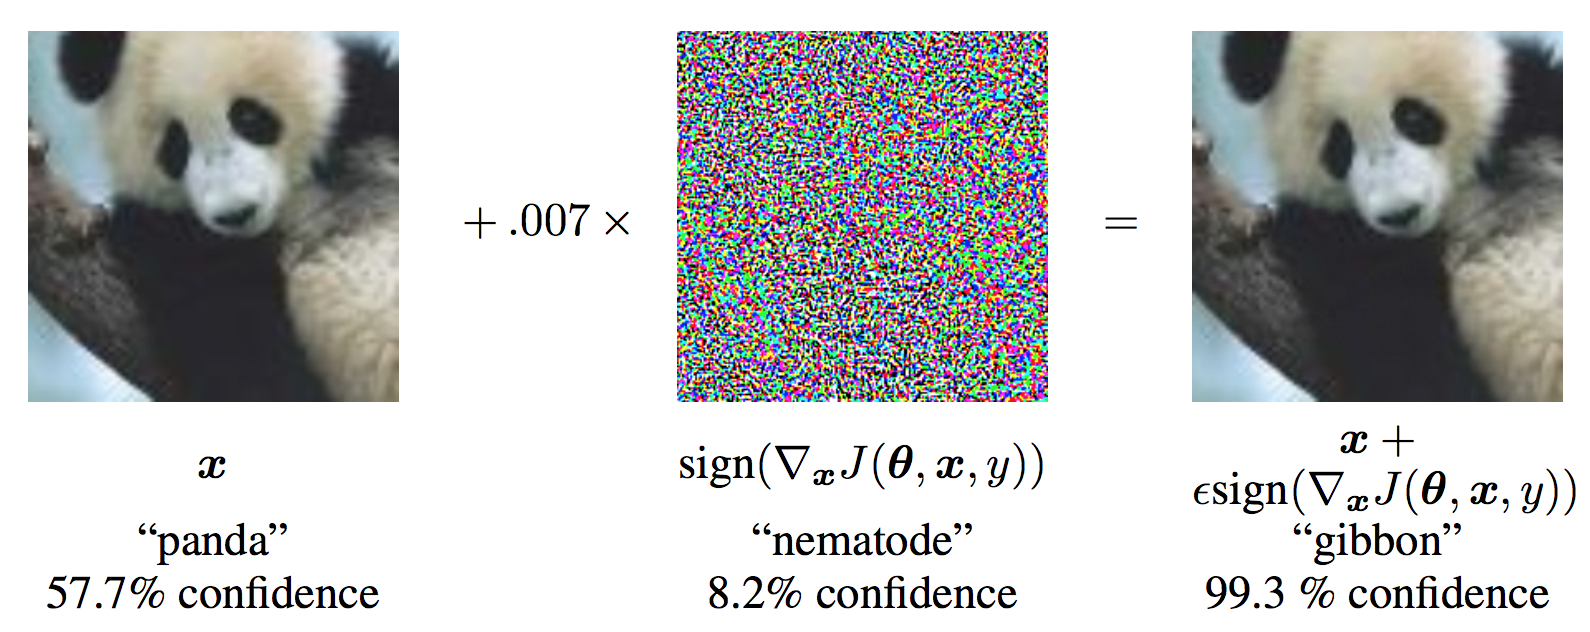
\includegraphics[width=1\textwidth]{figures/fgsm_panda_image.png}
\caption{FGSM adversarial image generation process, \( \epsilon = 0.007 \) (image taken from original FGSM paper)}
\label{fig:fgsmpanda}       % Give a unique label
\end{figure}

It is important to say that FGSM model is a adversarial attach whose purpose is a simple general misclassification method rather than a targeted method whose purpose would be to specifically make the model select a wrong targeted class.

FGSM is easy to implement, reference implementation from the PyTorch documentation was used for these experiments. FGSM only has one hyper-parameter: \( \epsilon \) which controls the multiplication factor of the gradient noise added to the input image. It is very similar to learning rate in gradient descent when using normal training techniques.

The results of the experiment with various \( \epsilon \) values can be seen in Table \ref{tab:results-fgsm} and Figure \ref{fig:fgsm_chart}. We can see that for every \( \epsilon \) value most of the negative models outperform the traditional model of the same architecture meaning that the negative models presented here are more resilient to FGSM white box adversarial attack, a result we were hoping for.

\begin{table}[ht]
  \centering
  \begin{tabular}{rS[table-format=2.1]S[table-format=2.1]S[table-format=2.1]S[table-format=2.1]S[table-format=2.1]S[table-format=2.1]}
    \toprule
     \textit{\(\epsilon\)/Model} & SN & ONN & HN & NR & ALT \\
    \midrule
    {(control) 0.0} & {98.79} & {98.78} & {98.92} & {\textbf{98.98}} & {98.92} \\
    {0.05} & {93.70} & {94.42} & {94.99} & {\textbf{95.07}} & {94.61} \\
    {0.1} & {77.34} & {80.09} & {80.88} & {81.35} & {\textbf{81.96}} \\
    {0.15} & {47.23} & {52.51} & {49.80} & {53.07} & {\textbf{55.65}} \\
    {0.2} & {20.39} & {23.99} & {20.41} & {24.72} & {\textbf{25.95}} \\
    {0.25} & {6.77} & {8.26} & {6.35} & {\textbf{8.99}} & {8.44} \\
    {0.3} & {2.71} & {2.65} & {2.15} & {\textbf{3.31}} & {2.40} \\
    \bottomrule
  \end{tabular}
  \caption{Results with accuracy for all models against FGSM white-box attacks. Bold are the best models per adversarial dataset. Please note that the control results are slightly different than before as normalization of the dataset has been omitted as suggested by the authors of the FGSM attack. Best models in bold.}
  \label{tab:results-fgsm}
\end{table} 

\begin{figure}
    \centering
    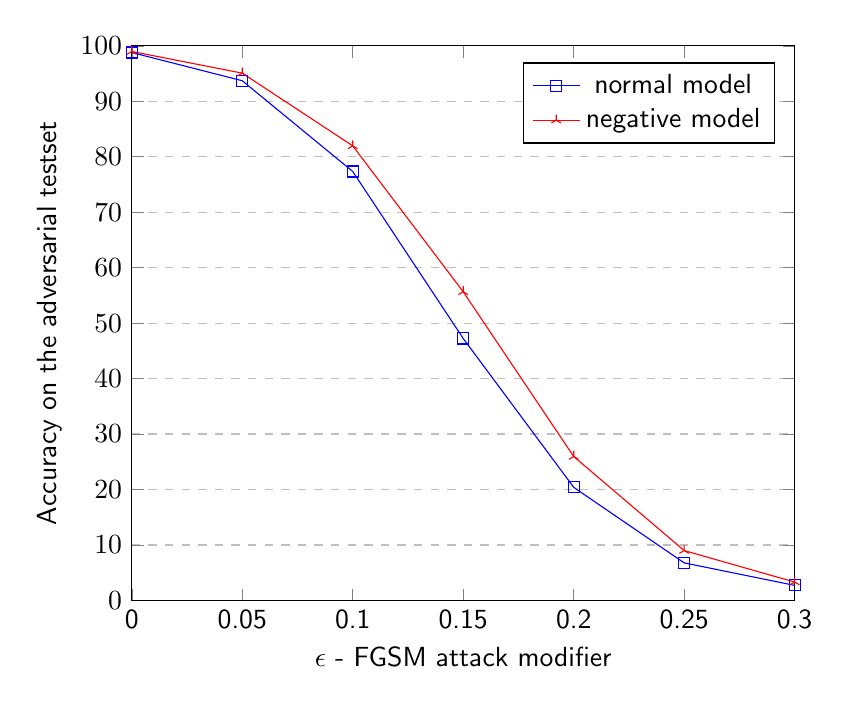
\begin{tikzpicture}
    \begin{axis}[
        xlabel={\(\epsilon\) - FGSM attack modifier},
        ylabel={Accuracy on the adversarial testset},
        xmin=0, xmax=0.3,
        ymin=0, ymax=100,
        xtick={0,0.05,0.1,0.15,0.2,0.25,0.3},
        ytick={0,10,20,30,40,50,60,70,80,90,100},
        legend pos=north east,
        ymajorgrids=true,
        grid style=dashed,
        xticklabels={0,0.05,0.1,0.15,0.2,0.25,0.3}
    ]
    
    \addplot[
        color=blue,
        mark=square,
        ]
        coordinates {
        (0,98.79)(0.05,93.70)(0.1,77.34)(0.15,47.23)(0.2,20.39)(0.25,6.77)(0.3,2.71)
        };
        \addlegendentry{normal model}
        
    \addplot[
        color=red,
        mark=Mercedes star, % lewis hamilton bre
        ]
        coordinates {
        (0,98.98)(0.05,95.07)(0.1,81.96)(0.15,55.65)(0.2,25.95)(0.25,8.99)(0.3,3.31)
        };
        \addlegendentry{negative model}
        
    \end{axis}
    \end{tikzpicture}
    \caption{Accuracy of normal and negative (best chosen) models against FGSM}
    \label{fig:fgsm_chart}
\end{figure}

\subsection{Black-box attacks: Black box Projected Gradient Descent attack on the negative models}

In contrast to the white-box adversarial attacks black-box attacks do not have direct access to the attacked network parameters. Instead they use different data to learn how to manipulate data in a way so that it is misclasified. One common way to use black-box attacks is to use a donor neural network (sometimes called a Holdout network) which the attacking algorithm studies and tries to figure out ways to manipulate it. Then this adversarial data generated based on the Holdout network is used in adversarial attacks on other networks. One algorithm that can be used in both white-box and black-box scenarios is the Projected Gradient Descent (PGD) \cite{madry2017towards} adversarial attack. It is normally used as a black-box algorithm with Holdout and Target networks but it can also be used as a white-box algorithm if both networks are the same. PGD attack is very similar to the previously used FGSM attack as it uses gradients from the Holdout network to try and maximize the loss function and in that way create adversarial examples which are wrongly classified. The difference between PGD and FGSM is that PGD limits the size of the perturbation (e.g. number of pixels) to keep the changes local and direct while the FGSM changes the entire input sample. The advantage of changing only local parts of the image is that it is more likely that humans will still be able to classify the input image correctly as only one part of it is changed. Another benefit of this approach is in generative models where we can actually deduce what are the differences in input data between specific class. For example if we have dataset of images of animals, PGD will be able to learn that if a beak is added the image will be classified as an image of a bird. If used in this way, PGD can provide us with the most important features of a class in dataset.

We experimented with black-box PGD attack where we gave it all of our five models for experimentation (one normal, four negative) as a Holdout model. Then with the adversarial examples generated, we compare all the accuracies on the adversarial testing datasets, results and comments in Table \ref{tab:results-pgd}.

\begin{table}[ht]
  \centering
  \begin{tabular}{l|ccccc}
    \toprule
     \textit{Holdout/Target} & SN & ONN & HN & NR & ALT \\
    \midrule
     SN & \textit{{29.28}} & {54.86} & {52.67} & {57.80} & {60.95} \\
     ONN & {52.62} & \textit{{33.33}} & {56.14} & {58.05} & {62.38}  \\
     HN & {48.58} & {53.83} & \textit{{31.68}} & {56.74} & {56.61} \\
     NR &{51.31} & {53.62} & {54.75} & \textit{{35.81}} & {59.27} \\ 
     ALT & {50.56} & {54.38} & {51.01} & {55.22} & \textit{{37.70}} \\
    \midrule 
     Avg. acc. & {44.47} & {50.00} & {49.25} & {52.72} & {55.39} \\
    \bottomrule
  \end{tabular}
  \caption{Results with accuracy for all models against PGD black-box attack. On the diagonal in italic font are the actual PGD white-box attack accuracies (same Holdout and Target model). We can see more severe damage caused by PGD in these cases. These results are taken for the middle epsilon value: \(\epsilon = 0.15 \). The last row presents average accuracies when using different models as target models, where we see again the negative models outperforming the normal model. The results are generally better for greater \(\epsilon\) values. Full results are available in the code repository.}
  \label{tab:results-pgd}
\end{table} 

\part{Synergy of Traditional and Classification Based On Missing Features}
\chapter{Overview of Ensemble Learning Techniques}

In the previous part of this dissertation we have shown and experimented with a new type of learning applicable to all convolutional neural networks: Classification Based on Missing (low-impact) Features. In the case of partial inputs/image occlusion, we have shown that our new method creates models that are more robust and perform better when compared to traditional models of the same architecture. In this part we explore an interesting characteristic of our newly developed models in that while we see a general increase in validation accuracy we also lose some important knowledge. Then we propose one discovered solution to overcome this problem and validate our assumptions against CIFAR-10 image classification dataset which has more complexity than the previously used MNIST dataset.

Ensemble Learning is a process in which multiple machine learning models are used for a single task. The reason for doing this is that with more than one model we can have more than one "opinion" and therefore we have greater probability that the ensemble model as a whole will perform better.

The simplest example is the Random Forest machine model which uses many decision trees and a voting system in classification and regression tasks. By not limiting the model to a single decision tree, we can learn much more information about the patterns in the training data and incorporate that knowledge in different sub-systems (decision trees) \cite{russell2002artificial} of the ensemble learning model.

Ensemble Learning can also be used in Deep Learning. One good example is in the multi-modal systems, where we need to make some decision or recognize some pattern based on different heterogeneous data. For example if we have a model which accepts an image and text describing that image and we want to output whether the description is correct we would need to use a multi-modal neural network system. In a such system one model would be used for processing the image and another one would be used to process text. Together, they would then produce some output. This has many benefits, the most obvious one is that we can use different type of neural networks for different tasks which can mean that we have increased performance. It is much better to use a recurrent model for text and a convolutional model for images (this is just one example) rather than one singular fully-connected model.

Our synergy network \cite{milosevic2020synergy} described here takes inspiration from ensemble learning models and the Siamese neural network model. In synergy networks as we will see, we have two models working in parallel. These models share some weights and have the same architecture but one of them is a negative model while the other is the "positive" or a normal neural network model.

Some experiments with joining multiple networks in the synergy models \cite{jasmina} and partial input and adversarial input classification \cite{mihailo} were performed as parts of two offspring MSc theses written by Jasmina Gajčin and Mihailo Ilić in 2020. Even though results and implementations from those manuscripts were not used in this thesis I thank them for their contribution and work on these tasks and hope we continue our collaboration.

\chapter{Synergy model}

In our work we already tested and empirically proved that our way of negative feature representation is suitable for training neural network models without any loss in accuracy. Moreover, we tested our models in one difficult scenario where algorithm robustness is important (object occlusion/partial inputs) and observed significant increase in accuracy. On the MNIST \cite{lecun1998mnist}, EMNIST \cite{cohen2017emnist} and our newly introduced PMNIST (partial MNIST) datasets of grayscale images of handwritten letters and digits we saw overall improvements in accuracy with some test cases having large increases e.g. \( 12.20\% \) increase in accuracy on the vertically cut (50\% image missing) PMNIST validation set. 

The intuition behind our solution is that by training the classifier to classify on negative (missing, low impact) features we obtain a more robust model in scenarios where some input features are missing. This makes our models suitable for tasks where some sort of an input mask is present e.g. occlusion, corrupt inputs.

\section{The need for ensemble "synergy" models}

Upon inspecting our negative models we discovered an interesting property that led us to this new synergy model. When comparing the accuracies of normal and negative models of same architecture, trained in the same way with same hyperparameters, we saw similar accuracies when testing on unmodified test sets. This is expected, as both models converge quickly. In testing with partial inputs, even though we gained some accuracy (in some cases more than \(10\%\)), by inspecting which samples were correctly classified, we discovered that our new network was wrongly classifying some instances which were correctly classified by the unmodified network. Therefore, we have discovered that while our new models are overall more accurate, the accuracy gain is not absolute.

\section{Model description}
\label{model}

In our previous work \cite{milovsevic2019classification} we showed that by using a simple activation function modification between feature extracting part of a CNN (convolutional layers) and classification (fully-connected) layers we can change the training process so the model uses missing (low-impact) features for classification. The main idea and goal of our method is to invert the feature extraction part of the network so that we obtain what features are missing (or not of high importance) on an input sample. Feature set is a finite set of features limited by the network architecture. In most neural network models, the number of features can be calculated from the number of convolutional layers in the network and their parameters: filter (kernel) size, number of filters, pooling characteristics (stride, type, width and height to consider), convolutional characteristics (e.g. padding type) etc. Most importantly, the output of the feature extractor is the place where we modify the signal before it is propagated to the classifying part of the neural network. As we mentioned earlier, this is very similar to negating the convolutional filter, but easier to implement because we do not have to modify the convolutional layers of existing networks.

To overcome the loss of knowledge we discovered, we create an ensemble model of two networks, one traditional and one negative. Both networks have the same architecture and share the convolutional, feature extraction layers. As we discussed in previous parts, we want to use the convolutional layers from the traditional model, so that we know it is our modification of the learning process that leads us to accuracy gains. This required some effort to make sure that our training process is deterministic and also that some of the weights are shared between models. To clarify, the shared parameters between the models are the frozen convolutional layers obtained from an unmodified neural network. The usage of negative models without shared parameters has also been tested, but it is incomparable to the unmodified models because the convolutional layers (namely filter weights) are completely different. Since we want to focus on models that use classification based on negative features, we want to make sure that the feature extraction parts of the networks remain unchanged in all the testing scenarios.

A simplified architecture diagram can be seen in Figure \ref{fig:1}. The convolutional layers are shared while there are two sets of classification layers we are training. On the left, a normal unmodified set of layers is trained while on the right we have a feature negation operation before the fully connected layers. We refer to the left side of the network as the positive side and the right side of the network as the negative side. The negation of the feature embedding vector is explained in Section \ref{negation}.

% For one-column wide figures use
\begin{figure}
\centering
% Use the relevant command to insert your figure file.
% For example, with the graphicx package use
  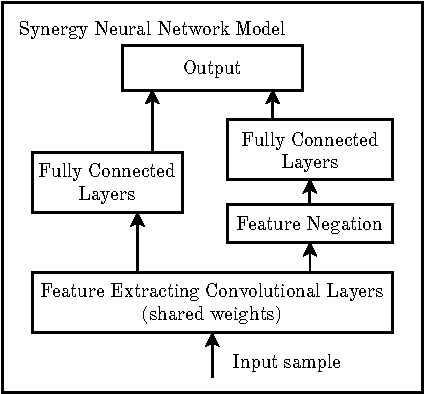
\includegraphics[width=0.4\textwidth]{figures/fig1.pdf}
% figure caption is below the figure
\caption{Synergy Model Architecture}
\label{fig:1}       % Give a unique label
\end{figure}

\section{Model architecture}
\label{modelarch}

To carry out our experiments we decided to use a well known and widely used neural network model. Even though our approach is viable for any convolutional neural network (or any model with a feature extraction part) we decided to test on a moderately complex neural network model from the PyTorch model library \cite{paszke2017automatic,paszke2017pytorch}. This model is well documented and known to work well with the CIFAR-10 dataset. The model is also fast to train which was useful in our testing. 

The used neural network model consists of five layers:

\begin{enumerate}
    \item 1st Convolutional Layer (\emph{conv1}), 3 input channels, 6 output channels, kernel size 5 x 5, 2D max pooling (\emph{maxpool}, kernel size 2 x 2, stride of 2)
    \item 2nd Convolutional Layer (\emph{conv2}), 6 input channels, 16 output channels, kernel size 5 x 5, 2D max pooling (\emph{maxpool}, kernel size 2 x 2, stride of 2)
    \item 1st Fully Connected Layer (\emph{fc1}), 400 input features, 120 output features (neurons)
    \item 2nd Fully Connected Layer (\emph{fc2}), 120 input features, 84 output features (neurons)
    \item Output Layer (\emph{fc3}), 84 input features, 10 output features (neurons)
\end{enumerate}

The forward pass through the network of the input sample (\emph{x}) can then be represented as seen in Equations \ref{eq:1} and \ref{eq:2}. ReLU activation function has been omitted from the equations for brevity. The ReLU activation function is used for fully-connected layers (\emph{fc1}, \emph{fc2}) and the convolutional layers (\emph{conv1}, \emph{conv2}).

\begin{equation}\label{eq:1}
conv(x) = maxpool(conv2(maxpool(conv1(x))))
\end{equation}

\begin{equation}\label{eq:2}
Fn(x) = softmax(fc3(fc2(fc1(conv(x)))))
\end{equation}

The hyperparameters were also defined and are as follows:

\begin{itemize}
    \item Loss function used is Cross Entropy Loss, suitable for problems of multi-class classification
    \item Optimizer used is Stochastic Gradient Descent with learning rate of \(0.001\) and momentum of \(0.9\)
    \item Batch size is \(4\)
    \item Number of epochs is \(10\)
\end{itemize}

We are aware that there are more performant, complex, deeper (and wider) models that can be used for this task, however we wanted to experiment with a model that we know can be improved and to do so without introducing more depth or width to the model. Our modifications to this model can be transferred to any CNN model, but this model was sufficient for our experiments because we want to show how to upgrade an existing model, without modifying its architecture. Later, we will also present results with modification of widely known ResNet18 \cite{he2016deep} model.

One similar architecture that we later discovered can be found in \cite{ganin2015unsupervised} where a model of similar architecture to our Synergy network is presented. In that paper a model where one feature extractor is used with multiple classification layers afterwards is very similar to our Synergy network model. More interestingly, the authors suggest the use of GRL (Gradient Reversal Layer) in a non-negative learning paradigm, but rather for multi-domain feature normalization. This approach could be of interest to us and possibly applicable to our negative learning approach. We will definitely explore this model and GRL in more depth in the future.

\subsection{Negating the features}
\label{negation}

In the negative network we use negation or inversion of the output of the feature-extracting convolutional layers. The process of obtaining the negative features depends on the output of the last convolutional layer in the convolutional blocks. Namely, it is very important which activation function is used in this last layer so we know what range of values we can expect as the output. We are using ReLU activation function throughout the convolutional layers of our models and the outputs are strictly positive values. Therefore we can calculate what features are missing (negative features) as they have very low, close to zero values. 

It is important to note that the negation function can also be applied to the convolutional kernel directly as we described previously, when introducing the negative model. As mentioned, in our approach we found it easier to apply the negation after the activation function since it is easier to work with only positive, scaled values. When ReLU activation function is applied, we can think of the output as the actual feature-positional vector where present features have high values and all the other features have values close to zero. It is yet to be determined if this approach is somehow different to our approach and if it can help with performance.

For our negative model, we have experimented with different negation functions \cite{milovsevic2019classification}, but have found that \( f(x) = 1 - x \) works best. When this function is applied to the squashed output feature vector, we obtain a new vector where negative features have values close to \(1\) and the present features have values either close to \(0\) or negative values. Either way, when these values are propagated through the following layers which also use ReLU activations, only the low impact (negative) features will be considered as they will have values close to one. It is important to note that the convolutional layers almost never output binary outputs with regards to whether a feature is missing or present. This is a shortcoming we hope to address in the future with further research regarding the negation process. When negation function is active, the forward pass through the network changes slightly compared to the normal network as can be seen in the Equation \ref{eq:3}. We emphasize that the convolutional part of the network is trained and reused from the normal network as can be seen in Equation \ref{eq:1}. The fully connected layers (\emph{fc1n}, \emph{fc2n}, \emph{fc3n}) are different (do not share weights with previous model).

\begin{equation}\label{eq:3}
Fneg(x) = softmax(fc3n(fc2n(fc1n(1 - conv(x)))))
\end{equation}

\subsection{Shortcomings of previous model}
\label{shortcomings}

In this section we further clarify our intentions with the synergy model and the shortcomings of the previously described negative model. Since the traditional (unmodified) model is still useful for some scenarios and shows good performance, we wanted to combine it with our new negative model so the knowledge loss is minimal. 

The conclusion that an improvement is possible came from a simple experiment we performed. After training and testing both models normally, base metrics of accuracy were obtained. As seen in Table \ref{tab:1}, both models perform similarly on the unmodified CIFAR-10 test set with our negative model slightly outperforming the traditional model. This test on the CIFAR-10 dataset also validates our previous results obtained on the MNIST dataset. 

\begin{table}
\centering
\caption{Performance of the negative and normal models}
\label{tab:1}
\begin{tabular}{lcc}
\hline\noalign{\smallskip}
Model & Validation Accuracy & Average Loss  \\
\noalign{\smallskip}\hline\noalign{\smallskip}
Normal CNN & 63.30 & 1.1513 \\
Negative CNN & 63.57 & 1.3377 \\
\noalign{\smallskip}\hline
\end{tabular}
\end{table}

The next step in our experiment was to see how many validation samples were correctly classified by both models. We expected that our negative model would correctly classify all the samples that the normal model correctly classified in addition to some new previously wrongly classified examples, but this was not the case. In Table \ref{tab:2} we see that our new model simply learned to classify some other input samples, and while the overall accuracy gain was present, this was not the desired behaviour since we want our model to be an upgrade over a normal model as much as possible. 

\begin{table}
\centering
\caption{Performance of the negative and normal models (case counts). CIFAR-10 validation set has 10000 images.}
\label{tab:2}
\begin{tabular}{lcc}
\hline\noalign{\smallskip}
Case & Occurrences \\
\noalign{\smallskip}\hline\noalign{\smallskip}
Normal CNN acc. & 6330 \\
Negative CNN acc. & 6357 \\
Normal CNN acc. \& Negative CNN inacc. & 1107 \\
Negative CNN acc. \& Normal CNN inacc. & 1134 \\
Both accurate & 5223 \\
Both inaccurate & 2536 \\
\noalign{\smallskip}\hline
\end{tabular}
\end{table}

\section{Training processes}
\label{datasettraining}

The training processes for our model are very similar to our previous experiments with the MNIST dataset. \cite{milovsevic2019classification} The first step in the training process is to train the normal, unmodified network. The training parameters have been described in section \ref{modelarch}. After the training of the normal model we freeze its convolutional layers because they are to be used in other models.

The second network we train is the negative network. The training process is the same as with the normal network apart from that the convolutional layers are already trained and loaded before training. In a way, we are performing fine-tuning of the network with the frozen convolutional layers from the normal network and with the negation operation activated. 
\subsection{Synergy network}
\label{synergy}

After we train the normal network and the negative network, we can join these models into a new model which we call synergy network. Synergy network is an ensemble of two networks of the exact same architectures, where one network is a traditional neural network model and the other one is a negative model. The simplified architecture diagram can be seen in Figure \ref{fig:1}. Both networks are already trained, meaning that creating the synergy network does not require additional training, rather just parameter copying. 

It is important to note how the ensemble of the networks functions -- or how the models are merged. For now, in our experiments we are using a simple addition of the probabilities for each class which are obtained from both neural networks (Equation \ref{eq:6}). The reasoning and the intuition for this is that we believe that there is an issue where the probabilities for the correct class and some incorrect class are very close in either the normal or the negative model outputs. Where we expect an improvement in accuracy is exactly in these cases. In these cases we are hoping that if an input sample yields very high output probability value for some class in one model (either negative or normal) while the other model outputs very close probabilities for two or more output classes, we will then consider the output class that the both models have strong confidence in. The forward pass through the synergy network can be represented with a set of equations (Equations \ref{eq:4}, \ref{eq:5}, and \ref{eq:6}). Please note that the convolutional block (\emph{conv}) is shared between all models and the fully connected layers have the same weights from models seen in Equations \ref{eq:1}, \ref{eq:2}, and \ref{eq:3}.

\begin{equation}\label{eq:4}
neg(x) = fc3n(fc2n(fc1n(1 - conv(x))))
\end{equation}

\begin{equation}\label{eq:5}
normal(x) = fc3(fc2(fc1(conv(x))))
\end{equation}

\begin{equation}\label{eq:6}
Fsyn(x) = softmax(neg(x) + normal(x))
\end{equation}

We have also thought of introducing a hyperparameter (\(\omega\)) giving preference to output of either of the two models. This new parametrized synergy network can be represented as seen in Equation \ref{eq:7} where the negative network influence to the synergy network output is dependant on the hyperparameter value.

\begin{equation}\label{eq:7}
Fsynp(x) = softmax(neg(x) * \omega + normal(x))
\end{equation}

In Table \ref{tab:3} we provide an example of some cases, where it is clear to see our intention with the synergy model. For the example (taken from the validation set) where normal network is incorrect and the negative network is correct we can see the output probabilities. The normal network has the highest confidence that the output class is class \(2\) (automobile), but also has relatively high probability for the correct class \(9\) (ship). The negative network has high probabilities for both these classes, but much higher for the correct class \(9\) leading to the synergy network outputting the correct classification result. In Table \ref{tab:4} we can see a similar case where the normal network is correct while the negative network is incorrect. The negative network, although incorrect, still outputs high probability for the correct class, again leading to the synergy network being correct.

The most extreme cases, of which there are \( 78 \) in our experiment, are those in which both networks are incorrect while the synergy network is correct. These cases are the most interesting ones as they represent an absolute increase in performance of our new joint model. In these cases, as seen in Table \ref{tab:5}, we have both networks yielding high probabilities for the correct class but even higher so for some incorrect classes. As both networks are wrong but not confident in their decision, the joint synergy model outputs the correct class.

In Figure \ref{fig:2} the three mentioned input images are shown and they are indeed difficult examples to classify, even to human eye.

It is extremely important to note that there are no cases where either of the networks outputs the correct class and the synergy model outputs the incorrect class meaning that we always have at least one model with correct classification and high confidence -- which is something we hoped to achieve. Also, from the given formulas it is also clear to see that if both networks are correctly classifying the sample, it is impossible for the synergy network to be outputting the wrong class.


\begin{table}
\centering
\caption{Cases when only one network is correct. Input sample is from the validation set (index \#2). C1 to C10 are output classes probabilities. Correct class is class 9 -- 'ship'. Rows represent three networks: normal CNN, negative CNN, and the synergy network which is the sum of the previous two. Bold is the highest probability, per network.}
\label{tab:3}
\tabcolsep=0.04cm
\begin{tabular}{lrrrrrrrrrr}
\hline\noalign{\smallskip}
 & C1 & C2 & C3 & C4 & C5 & C6 & C7 & C8 & \textbf{C9} & C10 \\
\noalign{\smallskip}\hline\noalign{\smallskip}
Nor. & 3.05 & \textbf{4.44} & -1.25 & -2.72 & -0.83 & -2.12 & -2.45 & -3.31 & 2.01 & 2.62 \\
Neg. & 6.04 & 7.29 & -1.39 & 0.11 & -6.85 & -8.49 & -9.60 & -4.89 & \textbf{11.55} & 3.22 \\
Syn. & 9.09 & 11.73 & -2.65 & -2.60 & -7.68 & -10.61 & -12.05 & -8.21 & \textbf{13.56} & 5.84 \\
\noalign{\smallskip}\hline
\end{tabular}
\end{table}

\begin{table}
\centering
\caption{Another case (\#7396) where normal network is correct whilst the negative network is incorrect. Correct class is class 9 -- 'ship'.}
\label{tab:4}
\tabcolsep=0.06cm
\begin{tabular}{lrrrrrrrrrr}
\hline\noalign{\smallskip}
 & C1 & C2 & C3 & C4 & C5 & C6 & C7 & C8 & \textbf{C9} & C10 \\
\noalign{\smallskip}\hline\noalign{\smallskip}
Nor. & 2.70 & 3.24 & -2.91 & 0.30 & -2.79 & -1.12 & -1.30 & -3.54 & \textbf{4.71} & 1.70 \\
Neg. & -1.12 & -0.95 & -2.21 & 2.19 & -1.12 & 0.26 & -1.79 & -1.23 & 1.96 & \textbf{3.16} \\
Syn. & 1.57 & 2.29 & -5.12 & 2.48 & -3.91 & -0.85 & -3.09 & -4.78 & \textbf{6.67} & 4.87 \\
\noalign{\smallskip}\hline
\end{tabular}
\end{table}

\begin{table}
\centering
\caption{One of the extreme cases (\#6418) where both networks are incorrect and unconfident, but synergy of the models outputs the correct result. Correct class is class 1 -- 'airplane'.}
\label{tab:5}
\tabcolsep=0.06cm
\begin{tabular}{lrrrrrrrrrr}
\hline\noalign{\smallskip}
 & \textbf{C1} & C2 & C3 & C4 & C5 & C6 & C7 & C8 & C9 & C10 \\
\noalign{\smallskip}\hline\noalign{\smallskip}
Nor. & 3.52 & \textbf{4.45} & -0.67 & -2.84 & 1.20 & -2.38 & -2.50 & -3.34 & -0.41 & 0.83 \\
Neg. & 4.00 & 2.63 & -0.31 & -0.16 & \textbf{5.22} & -2.03 & -1.94 & -2.73 & 0.42 & -1.30 \\
Syn. & \textbf{7.53} & 7.07 & -0.97 & -3.00 & 6.43 & -4.41 & -4.44 & -6.07 & 0.01 & -0.48 \\
\noalign{\smallskip}\hline
\end{tabular}
\end{table}

\begin{figure}
    \centering
    
\includegraphics[width=0.3\textwidth]{figures/fig2.png}
\caption{Input examples: \#2 (ship), \#6418 (airplane), \#7396 (ship)}
\label{fig:2} 
\end{figure}

\subsection{Other new models}
\label{other new models}

In our experimentation we are also introducing two additional models, useful for testing our changes. Both models are variations of the main synergy model.

Firstly, we introduce the "trained synergy" model. This is the model of the same architecture as the synergy model described in the previous section, joint of two parts: a traditional convolutional neural network and a negative network of the same architecture (Figure \ref{fig:1}) . The difference comes in the training process. This model is trained in a normal way, without any predefined parameters, for both the convolutional and the fully-connected layers. 

The idea behind this model is to test how parallel training of both parts of the network (normal and negative) will affect the end result. Since both networks are trained at the same time we are using information about both the present (high importance) and negative (missing, low importance) features as can be seen in Equation \ref{eq:6}. The propagated error, in this case, is directly dependent on the sum output of both of the networks. 

Another model we introduce is very similar, with the exception of using the convolutional layers from the normally trained network used for both models in the synergy architecture. We refer to this model as \emph{hot starting} trained synergy model. 

This model has a similar purpose to the previous one: to use both parts of the network during training. The difference here is to reuse the convolutional layers from other models we defined to stop any changes to convolutional kernels while training this way.

In the following section we will discuss more about our findings with both these models.

\section{Results and Discussion}
\label{results}

In this section we present the full results for all the models trained and tested on the CIFAR-10 dataset. In Table \ref{tab:6} we first present the validation accuracies of all the models. Please note that while the data is split into just training and validation sets, we are not performing any fine-tuning of the parameters based on the validation results. We are simply using the predefined parameters from the PyTorch code repository. This is why we felt that there was no need for a triple (train/validation/test) split of the dataset.

In the column Delta we see the difference between all the models and the normal unmodified neural network. First, we can see that our negative model which uses classification based on negative features outperforms the normal network by a very small margin. This increase in accuracy is not absolute -- we are not just correctly classifying \(0.27\%\) more of validation dataset, rather the correctly classified dataset subset is vastly different. Next model is the synergy network which is the best model we see here. As previously mentioned, the synergy network is not trained but rather a combination of the negative model and the normal model. We see a significant increase in accuracy when using this model on the unmodified validation dataset, and we will later demonstrate how the model performs on partial input data.

\begin{table}
\centering
\caption{Validation accuracies of the models. Accuracy is given as percentage. Column "Delta" represents the percentage difference between our models and the normal network.}
\label{tab:6}
\begin{tabular}{lcr}
\hline\noalign{\smallskip}
Model & Accuracy & Delta\\
\noalign{\smallskip}\hline\noalign{\smallskip}
Normal & 63.30 & - \\
Negative & 63.57 & 0.27 \\
Synergy & 66.98 & 3.68 \\
Trained Synergy & 63.32 & 0.02 \\
Trained Synergy (hot-start) & 64.28 & 0.98 \\
\noalign{\smallskip}\hline
\end{tabular}
\end{table}

Last two models, as described in section \ref{other new models} represent simple tests whether our approach is valid. The trained synergy proved that simply increasing the number of parameters is not enough. Both the trained synergy and the hot starting trained synergy models perform worse than the base synergy model as can be seen in Table \ref{tab:6}. The reason for this, we believe, is that during training the error is calculated and backpropagated on both the normal and negative parts of the network at the same time making it harder to converge. This is especially notable for the trained synergy model where we change a larger number of parameters (convolutional layers). 

Regarding training performance, normal and negative models were comparable in training time (with negative model being faster to train because of the copied frozen convolutional layers) while trained synergy models took longer because of the higher number of parameters to be calculated. The synergy network is not trained, therefore not comparable in training times to others.

\subsection{Testing with more complex models}
\label{resnet}

In this section we briefly display the results of our approach in training more complex models. The first architecture we tried is the ResNet18 \cite{he2016deep} neural network. First of all, we achieve very similar and comparable results to the one reported in the original paper. The implementation used was from the torchvision \cite{torchvision} library.

In Table \ref{tab:7} we see the results of testing with CIFAR-10 validation set. Even though our new models do not show meaningful increase in accuracy we are still considering this to be a good result because it shows that even in the case of very complex models of neural networks our approach does not negatively impact performance. 

When comparing the synergy model with the trained synergy model it is clear to see that it is not the architecture change that benefits the accuracy but rather our modified training process. 

Further testing with case-by-case analysis similar to what we present in this paper needs to be done in the future. We are looking forward to testing with other highly complex models and expect to find more substantial accuracy gains.

\begin{table}
\centering
\caption{Validation accuracies of the ResNet18 based models.}
\label{tab:7}
\begin{tabular}{lcr}
\hline\noalign{\smallskip}
Model & Accuracy & Delta\\
\noalign{\smallskip}\hline\noalign{\smallskip}
Normal & 92.52 & - \\
Negative & 92.48 & -0.04 \\
Synergy & 92.54 & 0.02 \\
Trained Synergy & 89.47 & -3.05 \\
Trained Synergy (hot-start) & 92.46 & -0.06 \\
\noalign{\smallskip}\hline
\end{tabular}
\end{table}

Please note that this model is not directly comparable to the main model presented in this paper due to major difference in architecture, hyperparameters, input processing and training characteristics. Full implementation is available at the code repository as described in Section \ref{source}.

\subsection{Testing with partial input samples}
\label{partial}

Since the main focus of our negative models \cite{milovsevic2019classification} was to increase robustness in the problem of partial input recognition, we also tested with partial inputs and present some initial results here. The tests were done with our synergy model, not with the ResNet18 based one. To test our new models we opted to test with removal of the lower left corner of test images to a certain degree. We have tested with removing up to \( 30\% \) of the input image. One example can be seen in Figure \ref{fig:3}. Even at this initial stage of testing we see very promising results. In Table \ref{tab:8} we can see that our main testing synergy model achieves the highest performance in all three validation sets. Most interesting result is in the C3 dataset with \( 30\% \) of the input image removed. There, our negative model actually performs worse than the normal network but the synergy network has strong increase in accuracy compared to the normal model, proving our initial hypothesis.

We have also tested another scenario, where we removed blocks of pixels from the input image. We created four new validation sets:

\begin{enumerate}
    \item Single Square Kernel (SSK) - one fixed position square removed
    \item Single Square Kernel Random (SSKR) - one randomly positioned square removed
    \item Multiple Square Kernel (MSK) - multiple (3) fixed position squares removed
    \item Multiple Square Kernel Random (MSKR) - multiple (2) larger randomly positioned squares removed
\end{enumerate}

The samples from these new validation sets can be seen in Figure \ref{fig:4}. The results of this test are shown in Table \ref{tab:9} where we can see similar behaviour to the previous test where corners of the images have been removed.

Similar to our previous work \cite{milovsevic2019classification}, it is important to note that these partial samples are not used during training, rather just for testing. We are eager to test with other input modifications and models in the future.

\begin{figure}
    \centering
    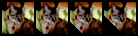
\includegraphics[width=0.7\textwidth]{figures/fig3.png}
\caption{Input example \#8 from CIFAR-10 validation set with various levels of occlusion added. From left to right: original image, \( 10\% \) removed, \( 20\% \) removed, \( 30\% \) removed}
\label{fig:3} 
\end{figure}

\begin{figure}
    \centering
    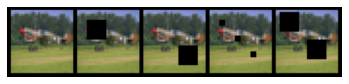
\includegraphics[width=1\textwidth]{figures/fig4.png}
\caption{Input example \#3421 from CIFAR-10 validation set with various modes of box occlusion. From left to right: original image, SSK, SSKR, MSK, MSKR.}
\label{fig:4} 
\end{figure}

\begin{table}
\centering
\caption{Validation accuracies of the models with testing with datasets with partial samples. C1 to C3 represent dataset with \( 10\% \), \( 20\% \), \( 30\% \) of the input image removed. Best results in bold text.}
\label{tab:8}
\tabcolsep=0.06cm
\begin{tabular}{lcccc}
\hline\noalign{\smallskip}
\emph{Model/Dataset} & Unmodified & C1 & C2 & C3 \\
\noalign{\smallskip}\hline\noalign{\smallskip}
Normal & 63.30 & 62.95 & 60.93 & 56.33 \\
Negative & 63.57 & 63.47 & 61.19 & 55.31 \\
Synergy & \textbf{66.98} & \textbf{66.51} & \textbf{64.33} & \textbf{59.08}\\
Trained Synergy & 63.32 & 63.22 & 62.29 & 57.29\\
Trained Synergy (h.s.) & 64.28 & 64.14 & 62.23 & 56.11\\
\noalign{\smallskip}\hline
\end{tabular}
\end{table}

\begin{table}
\centering
\caption{Validation accuracies of the models when testing with datasets with block removed partial samples. Best results in bold text.}
\label{tab:9}
\tabcolsep=0.06cm
\begin{tabular}{lccccc}
\hline\noalign{\smallskip}
\emph{Model/Dataset} & Unmod. & SSK & SSKR & MSK & MSKR \\
\noalign{\smallskip}\hline\noalign{\smallskip}
Normal & 63.30 & 54.04 & 56.89 & 61.15 & 47.60 \\
Negative & 63.57 & 51.27 & 56.15 & 60.38 & 45.08 \\
Synergy & \textbf{66.98} & \textbf{55.24} & \textbf{59.85} & \textbf{64.49} & \textbf{49.35}\\
Trained Synergy & 63.32 & 53.89 & 57.45 & 60.66 & 44.85\\
Trained Synergy (h.s.) & 64.28 & 52.73 & 54.37 & 62.00 & 46.27 \\
\noalign{\smallskip}\hline
\end{tabular}
\end{table}

\section{Experiments with different network joining techniques}

In synergy nets, one of the questions which needs to be answered is on model joining. In other words how can outputs of two models be joined and a single result produced. In our classification problem, both networks are created in such a way that they output probabilities, per-class for every known class in the dataset. So the output of both networks is a one-dimensional vector of length \( N \) where \( N = \text{number of classes in the dataset} \). These two vectors of probabilities need to be equally considered and joined so our joint model can make a prediction/decision.

\subsection{Addition}

The simplest way to join these two vectors, and in that way to join the two models: the negative and the positive one, is to use addition. To use addition we would sum the probabilities per-class. So the probability for the first class as an example would be \( p(c0) = p_p(c0) + p_n(c0) \), where \( p(c0) \) is the probability of the first class (we use zero indexing) and the \(p_p(c0)\) and \(p_n(c0)\) represent the probabilities from positive and negative networks respectably. We would do this operation for all the classes which in turn means that we are simply using element-wise addition of the both probability vectors as the output of the synergy net. This approach is currently used in the models we display here.

Several upgrades to this process are possible.

One upgrade would be to use a hyperparameter \( \omega = \) "importance of negative network"  which would control how both probabilities are taken into count when doing addition. With this parameter we can control the importance of both models, which could be useful in some scenarios where one network heavily outperforms the other one. If we are using this parameter the addition formula we mentioned before would be slightly different, in that the probabilities output from the negative network would be multiplied with the hyperparameter value: \( p(c0) = p_p(c0) + p_n(c0) * \omega \)

We have experimented with several values for the $ \omega $ hyperparameter. For this dataset/model combination the parameter does not seem to bring large differences in the results as can be seen in Table \ref{tab:omega05} and Table \ref{tab:omega20}. We will continue to experiment with this hyperparameter in the future, especially with regression tasks.

\begin{table}
\centering
\caption{Validation accuracies of the models when testing with $\omega = 0.5$. With this parameter value the normal network is two times more important than the negative network in the join process.}
\label{tab:omega05}
\tabcolsep=0.06cm
\begin{tabular}{lccccc}
\hline\noalign{\smallskip}
\emph{Model/Dataset} & Unmod. & SSK & SSKR & MSK & MSKR \\
\noalign{\smallskip}\hline\noalign{\smallskip}
Normal & 62.63 & 52.60 & 52.20 & 59.15 & 47.15 \\
Negative & 63.53 & 51.63 & 53.63 & 60.31 & 45.67 \\
Synergy & \textbf{66.28} & \textbf{55.82} & 55.79 & \textbf{62.98} & \textbf{50.63} \\
Trained Synergy & 63.70 & 55.48 & \textbf{56.76} & 60.95 & 47.93 \\
Trained Synergy (h.s.) & 64.46 & 54.05 & 54.89 & 60.65 & 47.31 \\
\noalign{\smallskip}\hline
\end{tabular}
\end{table}

\begin{table}
\centering
\caption{Validation accuracies of the models when testing with $\omega = 2.0$ where the negative network is twice the important when comparing it with the normal network.}
\label{tab:omega20}
\tabcolsep=0.06cm
\begin{tabular}{lccccc}
\hline\noalign{\smallskip}
\emph{Model/Dataset} & Unmod. & SSK & SSKR & MSK & MSKR \\
\noalign{\smallskip}\hline\noalign{\smallskip}
Normal & 62.36 & 52.46 & 51.66 & 58.69 & 47.45 \\
Negative & 62.95 & 51.97 & 53.37 & 60.22 & 46.14 \\
Synergy & \textbf{65.76} & \textbf{55.46} & 55.68 & \textbf{62.15} & \textbf{49.32} \\
Trained Synergy & 63.15 & 52.63 & \textbf{56.79} & 58.79 & 44.52 \\
Trained Synergy (h.s.) & 63.51 & 53.20 & 52.50 & 59.65 & 46.82 \\
\noalign{\smallskip}\hline
\end{tabular}
\end{table}



Another upgrade would be to divide the resulting probabilities with a number of networks from which they are sourced. This is not necessary if we are doing addition at the end of the model, since it is very likely that an \( argmax \) operation would be used for a final predictions. If however we need the final probabilities or they have to be used further in the model pipeline we would need to perform this normalization process: \( p(c0) = (p_p(c0) + p_n(c0)) / 2 \).

\subsection{Multiplication}

It is also possible, in a similar fashion to use multiplication instead of addition. It is clear that in this case the multiplication of the probabilities would bring higher confidence in the resulting model, without regard to accuracy. For example, if both networks output high probability for one class, its resulting probability would be exponential. And if models are in disagreement (one outputs high probability, other low) the resulting probability would be low. This means that the resulting probabilities would be high only if both models agree. We have experimented with multiplication and while it is possible to use it, it does not bring significant performance improvement in model accuracy as can be seen in Table \ref{tab:10}. While the synergy networks still outperform the normal network the performance is worse than the synergy network with normal addition. This can be seen when comparing Tables \ref{tab:9} and \ref{tab:10}. There may be another use case (dataset) or type of problem (e.g. sequence modelling) where this approach could lead to additional performance but it is yet to be tested.

\begin{table}
\centering
\caption{Validation accuracies of the models using multiplication when testing with datasets with block removed partial samples. Best results in bold text.}
\label{tab:10}
\tabcolsep=0.06cm
\begin{tabular}{lccccc}
\hline\noalign{\smallskip}
\emph{Model/Dataset} & Unmod. & SSK & SSKR & MSK & MSKR \\
\noalign{\smallskip}\hline\noalign{\smallskip}
Normal & 62.69 & 52.73 & 51.89 & 59.02 & 47.63 \\
Negative & 63.38 & 51.94 & 53.90 & 60.20 & 46.34 \\
Synergy & 56.24 & 45.70 & 44.21 & 52.30 & 41.09 \\
Trained Synergy & \textbf{64.27} & \textbf{53.36} & \textbf{55.20} & \textbf{60.48} & \textbf{48.38} \\
Trained Synergy (h.s.) & 56.21 & 46.69 & 49.27 & 52.21 & 38.40 \\
\noalign{\smallskip}\hline
\end{tabular}
\end{table}

\subsection{Separate join model approach}

Both addition and multiplication bring linearity to our model joining. But it is also possible to model the architecture in a way where we have non-linearity's. The easiest way to accomplish this is to use one or more fully connected layer (or other architecture) neural network before the final output of the model. This neural network model would consider (as its input) both the probabilities of the positive and negative models and would output the final probabilities. If we are to model the architecture in this way, we can then allow our model to learn specific information about both our models and their performance. One example would be that we can learn in what cases one model performs better than the other and what model to prioritize. Another possibility is to also give the final neural network model insight into the input data which both networks processed. Then, this model would be able to learn what model performs better in which case. It is important to note here that the synergy model would require small amount of training in this case, compared to the synergy model we described before, where the normal and negative models are simply joined.

We have experimented with various architectures for the joining model. We tested with one-layer fully connected networks, multiple layer fully connected network and convolutional networks. None of the models had significant (or any) improvement over our previously described approaches. When the joining model is learning it is difficult to outperform either the positive or the negative model, simply because they are already at their peak performance. The joining model only has information about the outputs of the two models and it cannot change them. In a way its performance is limited by the performance of the models being joined. Joining two models of similar performance cannot produce a model with additional performance.

We mention here the convolutional network with one-dimensional convolutions because it proved to work best. It is needed to explain why we believe using convolutions here can important. Rather than simply concatenating the output vectors we join them in a new tensor of dimension \( [batch\_size, 2, num\_classes] \). Two is the number of joining models. This way the relation between probabilities for specific classes are considered as they are neighbours in the resulting vector. When convolutional kernels (of size \( 2 x 1 \) setup specifically for this task) are processing the outputs of the two models they will consider this relationship and hopefully learn from it. The model in theory can learn patterns (e.g. for certain classes) in which a specific model is wrong and take that into consideration when making the final decision. 

In the Table \ref{tab:synergyfc} some initial results with one convolutional and one fully-connected layers added. While the accuracy changes are minimal, we can see that this approach is at least plausible. One benefit is that it also removes the need to choose what joining function needs to be used as it learned rather than chosen.

\begin{table}
\centering
\caption{Validation accuracies of the models when testing with datasets with block removed partial samples. Best results in bold text. Last row represents the newly introduced Synergy network with the additional layers at the end (SynergyF). The footer of the table represents the difference between the normal synergy and the upgraded SynergyF model.}
\label{tab:synergyfc}
\tabcolsep=0.06cm
\begin{tabular}{lccccc}
\hline\noalign{\smallskip}
\emph{Model/Dataset} & Unmod. & SSK & SSKR & MSK & MSKR \\
\noalign{\smallskip}\hline\noalign{\smallskip}
Synergy & 66.37 & 55.53 & 57.20 & 62.01 & 47.18 \\
SynergyF & 65.74 & 55.34 & 57.77 & 61.55 & 47.91 \\
\noalign{\smallskip}\hline
Delta & -0.36 & -0.19 & 0.57 & -0.46 & 0.73 \\
\hline\noalign{\smallskip}
\end{tabular}
\end{table}

\subsection{Neural Network Fusion in multi-modal systems}

% https://arxiv.org/pdf/1902.00038.pdf

The idea of joining several models with a smaller non-linear model which is usually a fully connected neural network comes from the definition of multi-modal neural networks. Multi modal neural network models need to operate on heterogeneous data where it usually makes sense to use different modelling for different data types. The best example is the VQA (visual question answering) problem where a model is presented with an image and a question about it. The response should be a label which represents a certain answer to the question. One example of BLOCK \cite{ben2019block} fusion architecture can be seen in Figure \ref{fig:block}, taken from \cite{ben2019block}. We mention BLOCK fusion here as a state-of-the-art network joining technique. BLOCK uses fusion based on the block-superdiagonal tensor decomposition  (block technique is know in the field of Signal Processing) and enables modelling very rich (i.e. full bilinear) interactions between groups of features, while the block structure
limits the whole complexity of the model, which enables to
keep expressive (i.e. high dimensional) mono-modal representations.

\begin{figure}
    \centering
    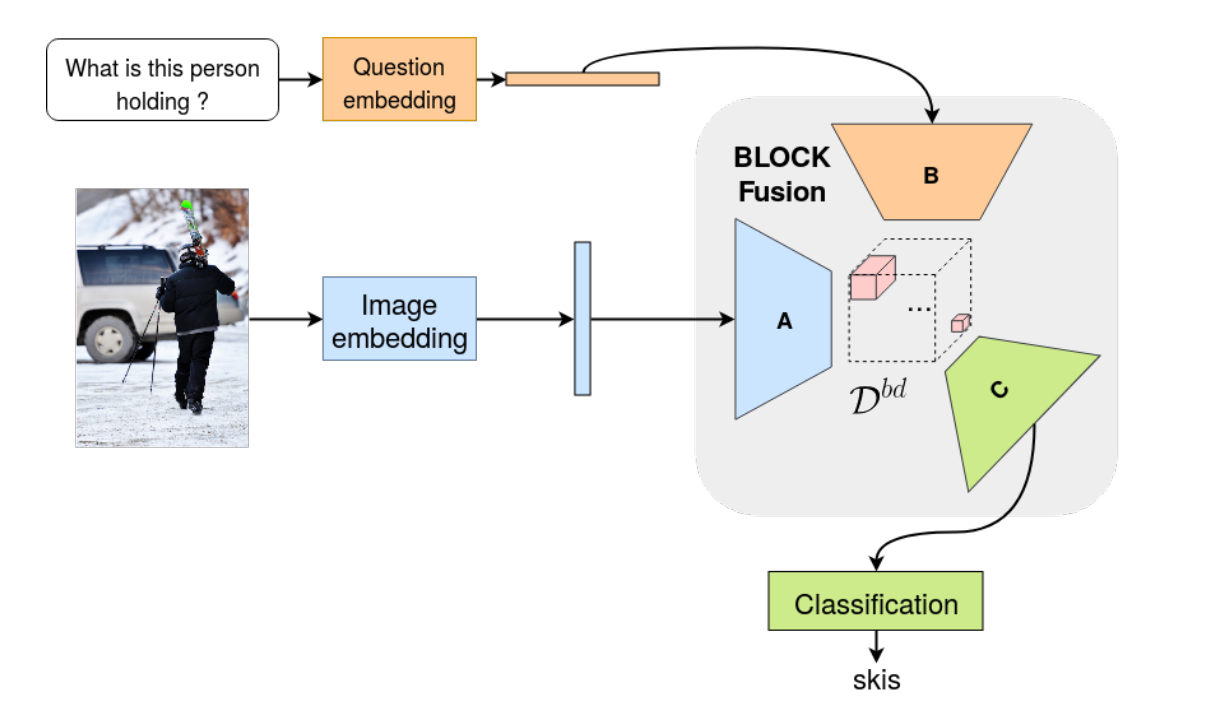
\includegraphics[scale=0.25]{figures/block.png}
    \caption{Example of Visual Question Answering architecture from BLOCK Fusion proposed method \cite{ben2019block}}
    \label{fig:block}
\end{figure}

We mention multi-modal architectures because these models need to employ different model joining techinques of which some may be useful to us even though so far our models operate on same type of data (images). 

The literature presents many ways of joining models:

\begin{enumerate}
    \item the two vectors are projected on a common space, and their summation is projected to predict the answer;
    \item the vectors are concatenated and passed at the input
of a 3-layer MLP;
    \item a bilinear interaction based on a count-sketching
technique that projects the outer product of between inputs
on a multimodal space;
    \item a bilinear interaction where the tensor is expressed
as a Tucker decomposition;
    \item a bilinear interaction where the tensor is expressed
as a CP decomposition;
    \item a bilinear interaction where each 3rd mode slice matrix of the tensor is constrained by its rank;
    \item a bilinear interaction where the tensor is expressed
as a Tucker decomposition, and where its core tensor has the
same rank constraint as (6);
    \item a higher order fusion composed of cascaded (6);
    \item BLOCK fusion \cite{ben2019block}
\end{enumerate}

In the future work these methods could perhaps be used instead of our proposed and tested methods described in previous sections. Some of the methods (methods 1 and 2) have already been tested here.

\section{Synergy Robustness to Adversarial Attacks}

In this section we revisit adversarial attacks, similarly to what we did in Section \ref{sec:adversarial}. We will repeat the experiments we did with the negative model, this time using the synergy model to see if it retains the robustness to adversarial attacks we found in the negative models. The one major difference is that this time we are testing with the CIFAR10 dataset, while we tested the older negative models with the MNIST dataset which also lets us see how the model robustness changes when the dataset is more complex.

\subsection{White-box attacks: Fast Gradient Sign Method attack on the synergy models}

First attack we experimented with is the FGSM method, the standard and most popular white-box attack where gradients of the model are used in combination with gradient ascent to make adversarial examples. We described this attack properties in more detail in Section \ref{sec:adversarial}. 

In the Table \ref{tab:results-fgsm-synergy} and Figure \ref{fig:fgsm_chart_synergy} we can see that the Synergy model outperforms the normal model by a moderate margin. One remark is that both these models (possibly related to the CIFAR10 dataset) are much more sensitive to the FGSM attack so the \(\epsilon\) parameter had to reduced in order to get meaningful results.

\begin{table}[ht]
  \centering
  \begin{tabular}{rS[table-format=2.1]S[table-format=2.1]S[table-format=2.1]}
    \toprule
     \textit{\(\epsilon\)/Model} & {SN} & {Synergy} \\
    \midrule
    {(control) 0.0} & {58.07} & {62.86} \\
    {0.005} & {42.12} & {45.95} \\
    {0.01} & {30.04} & {32.45} \\
    {0.02} & {15.47} & {16.13} \\
    {0.03} & {7.67} & {8.11} \\
    {0.04} & {4.25} & {4.70} \\
    {0.05} & {2.46} & {2.76} \\
    \bottomrule
  \end{tabular}
  \caption{Results with accuracy for both models against FGSM white-box attacks. Please note that the control results are slightly different than before as normalization of the dataset has been omitted as suggested by the authors of the FGSM attack. Synergy model outperforms the normal model in all test cases.}
  \label{tab:results-fgsm-synergy}
\end{table} 

\begin{figure}
    \centering
    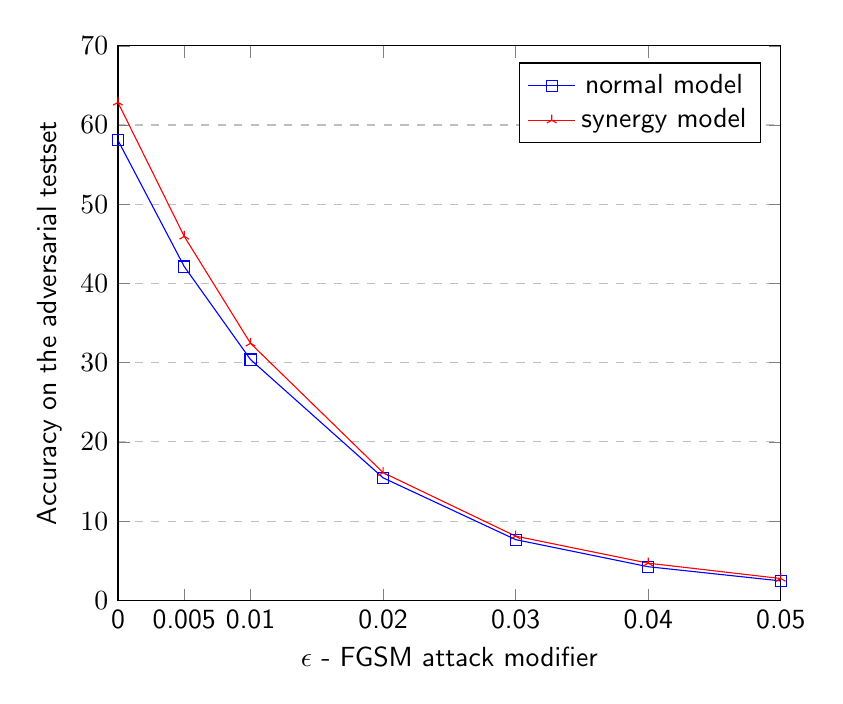
\begin{tikzpicture}
    \label{chart:fgsm_synergy}
    \begin{axis}[
        xlabel={\(\epsilon\) - FGSM attack modifier},
        ylabel={Accuracy on the adversarial testset},
        xmin=0, xmax=0.05,
        ymin=0, ymax=70,
        xtick={0,0.005,0.01,0.02,0.03,0.04,0.05},
        ytick={0,10,20,30,40,50,60,70},
        legend pos=north east,
        ymajorgrids=true,
        grid style=dashed,
        xticklabels={0,0.005,0.01,0.02,0.03,0.04,0.05},
        log ticks with fixed point,
        scaled x ticks = false
    ]
    
    \addplot[
        color=blue,
        mark=square,
        ]
        coordinates {
        (0,58.07)(0.005,42.14)(0.01,30.40)(0.02,15.47)(0.03,7.67)(0.04,4.25)(0.05,2.46)
        };
        \addlegendentry{normal model}
        
    \addplot[
        color=red,
        mark=Mercedes star, % lewis hamilton bre
        ]
        coordinates {
        (0,62.86)(0.005,45.95)(0.01,32.45)(0.02,16.13)(0.03,8.11)(0.04,4.70)(0.05,2.76)
        };
        \addlegendentry{synergy model}
        
    \end{axis}
    \end{tikzpicture}
    \caption{Accuracy of normal and synergy models against FGSM}
    \label{fig:fgsm_chart_synergy}
\end{figure}

\subsection{Black-box attacks: Black box Projected Gradient Descent attack on the synergy models}

We continue our testing with a PGD black box attack where we experimented both with using normal and synergy models as donor models for generating adversarial examples. We also use PGD as a white-box attack when selecting the same model as target and holdout, similarly to what we did in our experiments with the negative models.

In the Table \ref{tab:results-pgd-synergy} we can see the results when testing the models with PGD attack. In Table \ref{tab:results-pgd-synergy} we can see the results when using the normal model as the holdout (attacked) model and in Table are the results when using synergy model as holdout. Important metric is how the accuracy changes when either of the models is attacked.

\begin{table}[ht]
  \centering
  \begin{tabular}{l|cc|cc|c}
    \toprule
     \textit{\(\epsilon\)/Target} & {SN (SN)} & {Syn (SN)} & {SN (Syn)} & {Syn (Syn)} & BB Delta \\
    \midrule
    {} & {White-box} & {Black-box} & {Black-box} & {White-box} & {} \\
    \midrule
    {con. 0.0} & {58.07} & {62.86}  & {58.07} & {62.86} & {-} \\
    {0.005} & {31.12} & {41.24}  & {37.28} & {32.56} & {3.96} \\
    {0.01} & {18.24} & {28.32}  & {25.77} & {17.84} & {2.55} \\
    {0.02} & {2.42} & {6.71}  & {6.76} & {2.84} & {-0.05} \\
    {0.03} & {0.45} & {2.30}  & {2.89} & {1.49} & {-0.59} \\
    \bottomrule
  \end{tabular}
  \caption{PGD black-box (and white-box) attacks results for various \( \epsilon \) values when using normal and synergy models as the holdout model. First two columns are the result when using the normal (SN) network as the holdout whereas the last two columns show the results when using synergy network as the holdout. BB Delta column presents the difference of the models when using PGD as a black-box attack. Synergy network outperforms the normal network for \( \epsilon \) values smaller than 0.02 and is of very similar performance for greater values. At higher \( \epsilon \) values both networks performance is severely degraded.}
  \label{tab:results-pgd-synergy}
\end{table} 

\subsection{Other attacks}

In addition to PGD and FGSM attacks it is important to test other various versions and upgrades of the adversarial attacks for deep neural network. We can report that the synergy model performs well in these scenarios and outperforms the normal network in most environments. The robustness to adversarial attacks is a very wide field, so to keep the brevity of this document (and the sanity of its writer) we only present here white-box comparisons of the normal network and the synergy network for a fixed \( \epsilon \) value of \( 0.005 \). We test with the following algorithms:

\begin{itemize}
    \item PGD - Projected Gradient Descent (control for previous experiments) \cite{madry2017towards}
    \item BIM - Adversarial Examples in the Physical World \cite{kurakin2016adversarial}
    \item CW - Towards Evaluating the Robustness of Neural Networks \cite{carlini2017towards}
    \item RFGSM - Ensemble Adversarial Training: Attacks and Defences \cite{tramer2017ensemble}
    \item FFGSM - Fast is better than free: Revisiting adversarial training \cite{wong2020fast}
    \item TPGD - Theoretically Principled Trade-off between Robustness and Accuracy \cite{zhang2019theoretically}
    \item MIFGSM - Boosting Adversarial Attacks with Momentum \cite{dong2015image}
\end{itemize}

The results can be seen in Table \ref{tab:results-others-synergy}, default hyperparameters (from torchattacks \cite{kim2020torchattacks} library) were used.

\begin{table}[ht]
  \centering
  \begin{tabular}{l|cc|c}
    \toprule
     \textit{Attack/Target} & {Synergy} & {Normal} & Delta \\
    \midrule
    {PGD \cite{madry2017towards}} & {32.56} & {31.12} & {1.44} \\
    {BIM \cite{kurakin2016adversarial}} & {32.90} & {31.39} & {1.51} \\
    {CW \cite{carlini2017towards}} & {13.55} & {8.77} & {4.78} \\
    {RFGSM \cite{tramer2017ensemble}} & {88.56} & {85.65} & {2.91} \\
    {FFGSM \cite{wong2020fast}} & {35.90} & {33.79} & {2.11} \\
    {TPGD \cite{zhang2019theoretically}} & {54.30} & {50.66} & {3.64} \\
    {MIFGSM \cite{dong2015image}} & {34.51} & {32.64} & {1.87} \\
    \bottomrule
  \end{tabular}
  \caption{Synergy robustness to white-box state-of-the-art algorithms. Accuracy on the new generate adversarial test sets. Delta column represents the difference between normal and synergy models. Synergy model outperforms the normal model in all the tested adversarial environments.}
  \label{tab:results-others-synergy}
\end{table} 

\section{Short summary and conclusions for the Synergy models}
\label{summary}

In this part we discussed our discovery of some shortcomings of our classification based on missing features approach. Firstly, we validated our previous results on the more complex CIFAR-10 dataset and then experimented with introducing an ensemble synergy model of the traditional CNN and our negative CNN to further boost performance. In our experiments we have showed that there is definitely a possibility for more accurate models when using this approach. We have also shown where the increase in performance comes from -- the cases where one network is uncertain and the other is highly confident. In our initial testing with partial input data we also show that our modifications (that can be applied to any convolutional neural network) lead to notable accuracy gains in these cases without any major architectural changes.

While these models have only been tested on the unmodified CIFAR-10 validation set and the corner cut validation sets for now, our goal is to repeat our experiments for various types of occlusion in images. Another area where it is possible to improve is combination of the two models inside the synergy model. As previously described, we are only experimenting with simple probability summation although other approaches are definitely possible. We will also experiment with other ways of joining the networks, one being to add one or more fully connected layers which are given the outputs of the two networks as inputs. The \emph{trained synergy} models are also to be further examined. It is possible that with some parameter optimization, accuracy can be improved.

We have also considered combining our models with newer neural architecture search \cite{elsken2019neural} and genetic algorithm methods \cite{assunccao2019fast} to try and discover more models that can benefit from our changes.

Additionally, we want to experiment with more state of the art (e.g. \cite{he2016deep,huang2017densely,xie2017aggregated}) models which achieve very high accuracy on the CIFAR-10 and ImageNet \cite{deng2009imagenet} datasets. While our work in this paper focused on a simpler and easier to train model, we believe that the modifications described in this paper can also further improve even the most complex models of today. We are also eager to try our approach in regression tasks and we are already familiar with some application that could benefit from this approach \cite{pecev2016system,pecev2017ltr}.

\part{True Negative Deep Learning}

\chapter{Goals, motivation and implementations}
In this part of this PhD thesis we mainly present discussion and ideas for other, pure, negative deep learning models. While many of these models are still in their inception phase, we believe this path of research will yield in useful models for wide variety of scenarios. The general goal is to explore this approach to learning and what benefits it would bring while we also demonstrate some of our implementations and contributions.

The main problem with true negative learning models, as we will present, is the need for negative samples during training which are often difficult to obtain as they require really specific use cases or manual labeling of large datasets. While other approaches such as Negative Sampling which uses stochasticity for creating negative samples are possible we believe a more "natural" formulation is required. For image classification, for example, one useful scenario would be to have parts of the images humanly processed and negatively labeled. This means that humans would look into parts of images and deduce to which class they do not belong. This training data would then be used for negative training and hopefully be similar in performance to the normal model when the entire image is shown and outperform the normal model when only partial input is given as it would learn to generalize better. This approach brings an interesting concept which we hope to explore in the future: partial input training. In partial input training we give the network only parts of the input samples during training, but expect the network to also be able to classify whole input samples. In a way it is a similar approach to random-crop normalization in image classification tasks. This approach is interesting because it goes hand in hand with negative learning we display in this thesis. If parts of the images can be labeled as negative samples for certain classes this knowledge would, we strongly believe, help the network learn better representation of patterns in training data and to which classes these patterns do not belong, increasing overall performance of the negative models.

We also consider combination of normal training and negative training similar to our Synergy model and ALT model from before (Section \ref{altmodel}). From our experiments it is probable that negative learning can be used in combination with normal learning to further increase performance.

At this stage, we can demonstrate two concrete examples as proof-of-concept implementations which we developed: A negative Siamese Triplet-Loss Neural Network and a negative Deep Reinforcement Learning (DQN) agent. Other models mentioned in this part of the thesis are either our ideas for future work or some approaches we believe are related or can be modified slightly to employ negative learning.

In previous parts of this dissertation we described and focused on some specific models of negative learning which use special feature representations in order to deduce the output class in classification tasks. In this part we will discuss potential and existing implementations of "true negative learning". With the term true negative learning we consider models which do not use special feature representation but rather modified data and/or training process to implement negative learning. In other words these model learn by recognizing patterns in the form of what is not the output class based on the input data, where our models used unmodified input data for a similar purpose. There exist several models which implement similar patterns and we will discuss them in this part of the manuscript.

Goals of the true negative deep learning model is similar to the models we have already seen. To learn additional information about the data based on negative patterns in the data which can be missing information or the actual negative labels (e.g. what something is not in classification tasks). This way of learning can be implemented in several ways and there are already several models which use something similar. In this chapter we will mention two groups of true negative deep learning models. The first group is the models which work by modifying the dataset (e.g. negative sampling) and the second group is the models which are using other techniques (e.g. loss function modifications).

\section{Gradient Ascent Variation}

Firstly we mention Gradient Ascent as the main idea behind "true negative learning" models. Gradient Ascent is a known modification of the Gradient Descent optimization algorithm. 

In Gradient Descent (and its variations, e.g. Stochastic Gradient Descent) a model is optimized by minimizing the value of a certain loss function which describes how the model is performing. The loss function is formulated so that the output value is higher for higher error rate, or in other words the smaller the value the better the model is performing. In some literature this process of minimization of the loss function is called "walking the gradient" which explains the iterative nature of the algorithm (small steps towards the minimum of the loss function).

Gradient Ascent is very similar to Gradient Descent but with one major modification in that we walk the gradient uphill, maximizing the loss function. 

Making the loss function output higher values may look like simply trying to modify the model weights so the error rate is higher, and this is true to some extent. We have already seen several examples where Gradient Ascent is used in adversarial attacks, FGSM attack for example. But Gradient Ascent, we believe, can also be used for negative learning, in combination with Gradient Descent. We will now describe how we think this can be achieved.

This neural network model can be trained in two ways: normally until the model converges and no further updates yield better performance and then fine-tuning it with negative learning, or, by incorporating negative learning during the main training process. It is important to note that we also consider using various combinations of positive and negative training. We already showed that one such model is sometimes outperforming other negative models and that is the ALT model from Section \ref{altmodel}. In that model we use negative and positive learning process in variation and that model shows that there is a possibility that this combined approach can be beneficial. 

One example which is easy to imagine is if the network becomes stuck in a local minimum while learning. In that scenario it would perhaps be possible to use negative learning for a number of steps to force the network to overcome this local minimum as the loss function space would change its shape entirely. 

Apart from helping with this problem, it is possible that this way of combined training can help in other areas such as training time. We could, for example, train first with only negative samples which would for some datasets allow the network to learn faster and then fine-tune the network with normal training. We could also try to randomly choose during training whether normal or negative training is used, which could also aid in convergence times. 

Another important thing to mention here which could also be relevant is the ratio between positive and negative training samples. For now we mostly focus on fine-tuning our models with a small number of negative samples, but it remains to be experimented whether using higher percentage of negative samples during training will help with performance somehow.

For any version of the Gradient Ascent approach, we would need negative input samples, which in a m-ary classification problem would be inputs for which we know they do not belong to a specific class (or a set of classes). In image classification problems for example, we would define a negative input sample as an image or a specific part of the image for which we want to tell our model to specifically care about not belonging to a specific class. One good example can be seen in the Figure \ref{fig:sample-motivation} which we used to introduce the CBOMF model in previous parts of this thesis. There, the presented missing features are a good candidate to use as negative input patterns because for these patterns we know specifically to which class they do not belong. When a negative pattern is presented to the model we would use Gradient Ascent to reduce the weights and biases of the network leading to the negative output class. In other words, we would walk uphill on the gradient away from the output class, or "pull away" from it. 

This can help in different scenarios such as the demonstrated one where parts of the input are missing. It could also help with situations where network misclassifies two similar classes in a more complex dataset. We could use the training data in combination with confusion matrices to see what classes are often misclassified as other classes, sample from the data and create negative samples for these cases.

This learning step can be achieved in at least three ways which are simple to implement. We already mentioned the first way, which is to use gradient ascent without further modification to the data. Secondly, we could invert the desired output of the negative pattern. The output in the classification task would be an inverted vector where we would have the opposite values of the one-hot vector used during training. If done so, the weights and biases are changed during training so that the parameters leading to the negative output class are reduced and the parameters leading to other classes are increased. The third way to achieve this is to invert the gradients during training with negative samples, without changes to the data. This can be achieved by employing negative learning rate values or by specifically negating the gradients in the backwards pass.

We would like to emphasize that the main goal for these models is, similarly to other negative models, to achieve higher performance by providing additional knowledge. Here, this additional knowledge would be specific negative input patterns which exist naturally or are synthetically made to aid the network. For example, if we have a model which often misclassifies two specific classes we could provide additional negative samples so the network learns that if a certain pattern is observed in the input sample what the output class is not. 

We present this model only as an idea in this thesis, hoping to implement it and evaluate it at a future time. While the implementation would be moderately difficult, the main task or issue is finding a suitable dataset or manually creating negative input samples. An useful idea there is that it is perhaps possible to generate negative samples by randomly selecting parts of the input patterns while also randomly choosing a negative class to which they do not belong. Problem with this approach is the randomness of the process which would bring instability. For example, we cannot be sure that the randomly chosen input pattern is important for a specific class just as we cannot be sure that the input pattern is a "negative" example for some other class. One somewhat similar approach is presented in the following section. 

In our Negative Triplet-Loss Siamese model we will see a similar approach to the Gradient Ascent we mention here. In Siamese models it is easier to control the negative learning process as it is built in the model by using metric (similarity) learning.

\section{Negative sampling}
\label{negsampling}

In this section we describe negative sampling as a form of negative deep learning knowledge. Negative sampling is a process of transforming a dataset in a way to generate negative or wrong examples. In m-class classification problems this can be done in several ways. The simplest way to generate negative samples is to use the following process: for every sample in a dataset choose a random label which is not equal to its actual label. This process can be repeated many times to generate even more negative data. This data at first may seem to be not important, but for negative models it represents viable and important knowledge. Another way to use negative sampling is to choose a specific negative class for a sample we are observing. This can be useful in some scenarios, for example to overcome bad performance on two (or more) specific classes which are often very similar in classification. Problem with this approach is that it often requires manual labeling.

In the second case, manual labeling can be avoided if we use several models for training. For example, we train one model and observe its results on a subset of data from the validation set. In these results we can notice some classes in the confusion matrix where the model is often confused in classification. Then we can use that information to generate negative samples for our second negative model which will use this additional knowledge of "problematic" classes in our dataset and hopefully overcome them.

\section{Noisy Label Classification}
\label{noisylabels}

Where negative learning models showed promise is in the problem of noisy label classification. Having dataset with clean labels is very rare in real world scenarios, and even datasets which are used commonly for neural network training (e.g. MNIST, CIFAR) have wrongly classified samples in them. These samples we called noisy samples or samples with noisy labels.

During production of this dissertation, a lab from South Korea has also been experimenting with negative models for tasks of noisy label classification. \cite{kim2019nlnl} In the paper they use Negative learning models (with random negative sampling as described above) to train models more robust to noisy labels. In the paper CNNs are trained using a complementary, synthetic label as in "input image does not belong to this complementary label". The main premise is that for noisy label classification negative samples provide wrong information much less frequently than normal unmodified data. This prevents the network from overfitting or remembering the wrongly labeled data.

Their approach has some, albeit small similarities to the methods presented in this dissertation. First of all, the models described in the paper only concern robustness to noisy labels not general robustness of the model to input modifications or adversarial attacks as we experimented. They also use negative sampling to generate negative samples for training and a simple modification to the loss function where the softmax output of the network is inverted (all classes have probability value 1 apart from the actual class which has a value of 0). They also experiment with a combination of positive and negative learning models (with somewhat similar goals like our synergy network) to overcome bad performance on cleaner datasets without noisy labels where normal, positive models outperform negative models. This method can be used also for data filtering so that noisy labeled data can be removed from the dataset used later on.

In the paper it is demonstrated that the introduced negative models and negative sampling in general can help in creating models more robust to noise in the label data, both artificially added and the actual noise in the datasets, another use case for the negative models related to robustness.

It is very possible that the models introduced in this paper could also be useful for classification of partial or adversarial examples but this remains to be tested at a future time. We will demonstrate our approach to "pure" negative training with Siamese Neural Networks where the gradients are actually "pulled away" from the negative class.

\section{Noise Contrastive Estimation Models}

Another negative model used most notably in Natural Language Processing is the NCE (Noise Contrastive Estimation) \cite{mnih2013learning} model.

This model tries to solve the issue of having large vocabularies in language tasks where huge neural network models are needed, even for simple tasks. 

One example would be in the next-word prediction tasks in which given a part of the sentence a model would be able to predict the next written word. This system is commonly used and needed for accessibility reasons or faster typing on for example mobile devices. It is also used in grammar checking software. The models for next-word prediction are trained on large corpuses of text. Before training the data is processed so that unique words are found. This step is important because vocabulary size defines the architecture of the model. If we have a densely connected network we need to have the output layer of size of the vocabulary where every output neuron represents a single word from the vocabulary. Then a softmax function is used to process the output vector and we then obtain the next word index and the word from the vocabulary. It is immediately apparent that this is an issue when we have large vocabularies as our network needs to be very wide, especially if we have multiple words as inputs. 

NCE models work differently in that they do not learn how to classify (this task can be looked upon like it is multi-class classification problem) but rather how to separate actual word pairs (word that are supposed to be together, positive samples) from the noisy pairs (negative samples). This is achieved by creating positive and negative input samples, where positive samples are all of the same lenght which is much shorter than the vocabulary and contain words found often together in the input text dataset. Negative samples are formed in the opposite way: words which are rarely used together are formed as negative samples. For NCE models it is very important to define the \(window\_size\) parameter which is used to define the length of the input data. NCE uses negative sampling to choose random words for the creation of negative input samples but some variants also use words least frequently used in pairs as an additional regularization technique (word2vec \cite{mikolov2013efficient}).

Most notable implementation of this algorithm is in the unsupervised learning word2vec \cite{mikolov2013efficient} algorithm. In this algorithm this method is used to generate word embeddings in a multidimensional space where words which are used together have similar embeddings -- they are close in the vector space. One example can be seen in Figure \ref{fig:word2vec}.

\begin{figure}
    \centering
    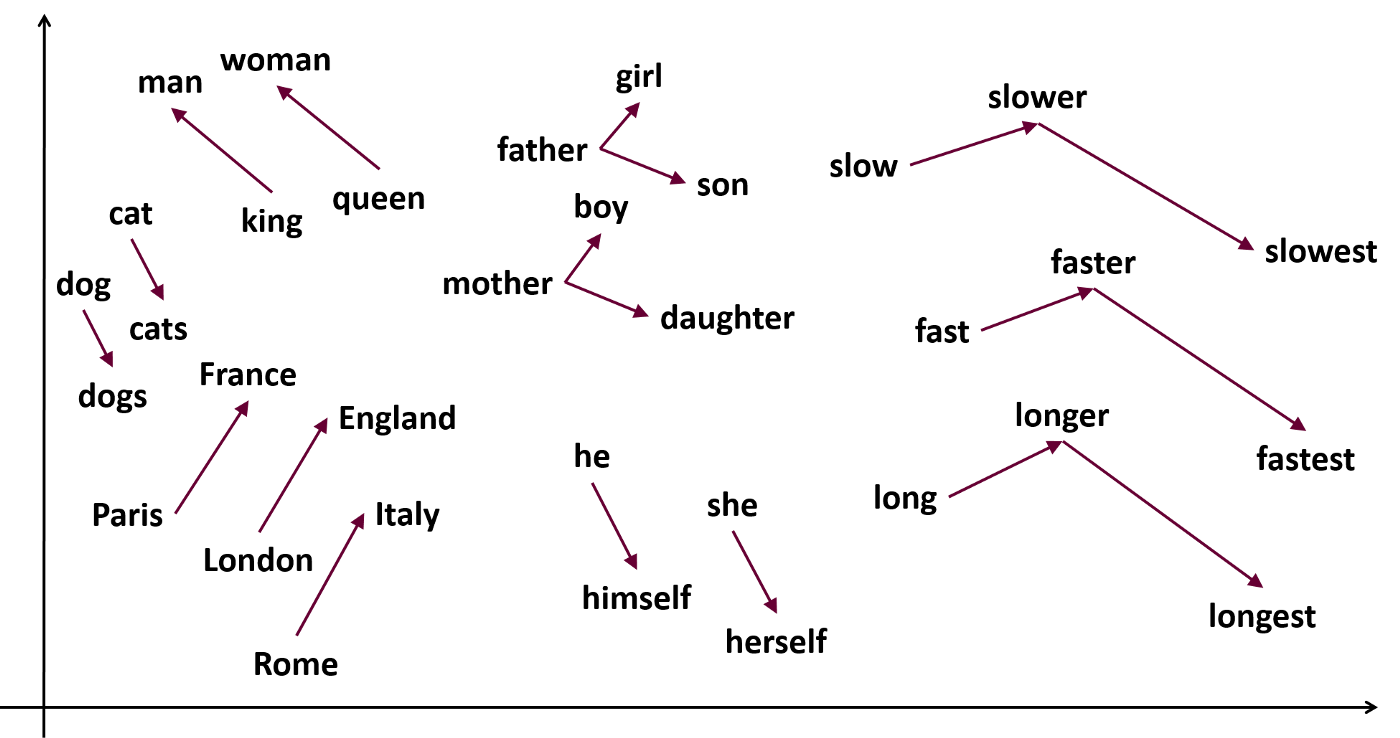
\includegraphics[scale=0.2]{figures/word2vec.png}    \caption{2-D space of English words generated with word2vec. Words with similar semantic meaning are close in the embedding space.}
    \label{fig:word2vec}
\end{figure}

The basic idea is to convert a multinomial classification problem (as it is the problem of predicting the next word) to a binary classification problem. That is, instead of using softmax to estimate a true probability distribution of the output word, a binary logistic regression (binary classification) is used instead.

For each training sample, the classifier is fed a true pair (a center word and another word that appears in its context) and a number of \(k\) randomly corrupted pairs (consisting of the center word and a randomly chosen word from the vocabulary). By learning to distinguish the true pairs from corrupted ones, the classifier will ultimately learn the word vectors --instead of predicting the next word (the "standard" training technique), the optimized classifier simply predicts whether a pair of words is good or bad.

word2vec \cite{mikolov2013efficient} slightly customizes the process and calls it negative sampling. In word2vec, the words for the negative samples (used for the corrupted pairs) are drawn from a specially designed distribution, which favours less frequent words to be drawn more often.



\chapter{Siamese Neural Networks and our upgrades}

Siamese Neural Networks \cite{koch2015siamese} are a special class of neural networks used in Similarity Learning. Where many networks used for classification use data to learn what patterns define a class and to recognize those patterns, Siamese networks learn to model a similarity function which simply can tell us if a certain input pattern is similar to another and how much similarity there is.

Siamese neural networks can be used for classification purposes if we have access to training data during inference also. In these cases when an input sample is presented we would simply try to find one similar to it in our training data and output the probability (similarity) that the class is the same. 

These models are called Siamese because they often contain two separate paths or two neural networks of same or similar architecture (similar to our synergy network) which are used for positive and negative processing. These models also often share weights. To clarify, not all Siamese networks use negative processing but it is certainly possible with a specific loss function, more details in the next section.

Siamese neural networks thrive in use cases where there is little data available. Often we need a lot of data to train neural networks to consider every possible input variation and situation, but in the case of Siamese networks, since we are only learning a similarity measure we can use less data to achieve similar goals. This is why these systems are used very often in face-recognition software where we usually have a single image of a person we need to recognize. They are also used for many other tasks: fingerprint recognition, signature verification, plagiarism detection, object tracking etc.

One more benefit of these models in comparison to other classification deep neural network is the ease of online training. One example would again be a face recognition system in an organization. When a new person is hired to some organization if we were using a normal neural network, we would have to retrain it, because the structure would have to different to accommodate the additional output class. If we are using a Siamese network model, this is not needed as we only need some additional training with the new data we have. 

There are some disadvantages to these models however. Because we need to compare the input to all the samples in the training dataset, inference times are usually slower than the traditional CNNs or fully-connected networks. These models also need regularization (weight decay is often used) to stop them from getting stuck in local minims. 

\section{Negative learning with triplet Loss Function and our modifications}

Siamese neural networks are often used with either Contrastive Loss \cite{melekhov2016siamese} or Triplet Loss \cite{dong2018triplet} functions as a criterion. Contrastive loss, learns embeddings in which two similar samples have a low Euclidean (or other) distance while two dissimilar points have a large Euclidean distance. These embeddings are not suitable for negative learning.

\begin{figure}
    \centering
    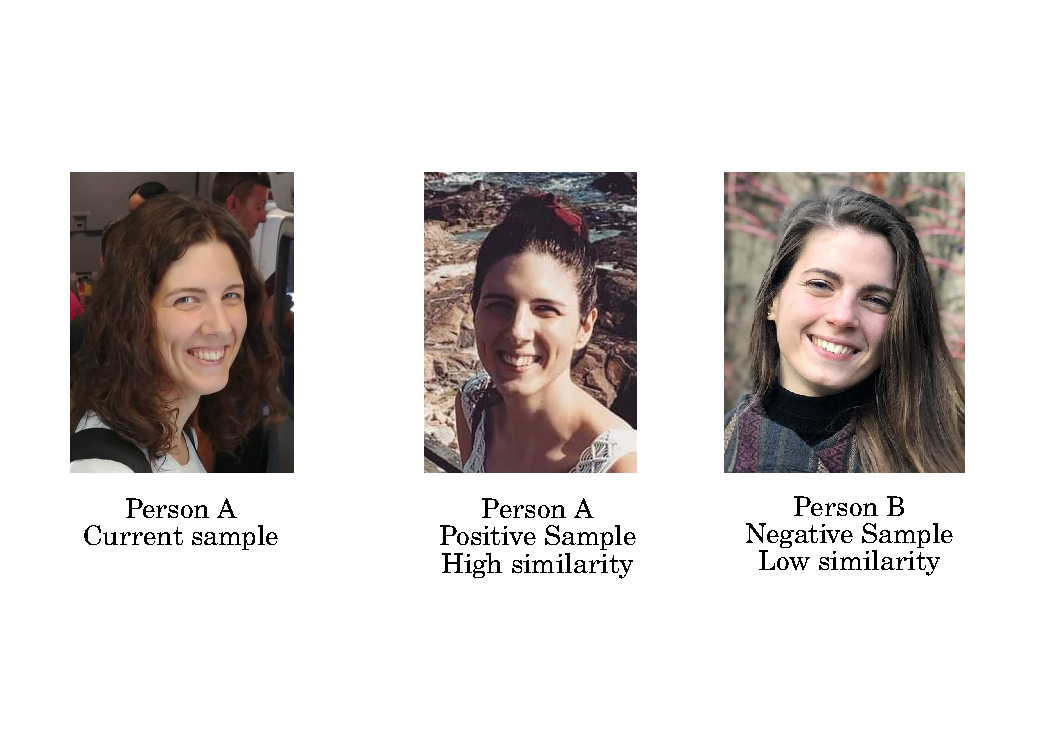
\includegraphics[trim=0.5cm 2.6cm 0.5cm 5cm,scale=0.73]{figures/siamese.pdf}
    \caption{Example of Face Identification Siamese Neural Network (e.g. \cite{varior2016gated}) training with triplet loss function. A triplet of data samples is used: current sample for which we are training, a positive sample of the same class and a negative example of another class. After embeddings are computed and the distances are calculated the optimizer of the model minimizes the distance between same class samples and maximizes the distance between the current sample and the negative sample.}
    \label{fig:siamese}
\end{figure}

Triplet Loss function uses an interesting concept of negative learning in that it uses negative samples as a regularizer. In triplet loss function, to compute a loss we need three input samples. The main input sample used for training, called the anchor is compared with two other samples from the dataset. The first comparison is between the anchor and a random positive sample and the second comparison is between the anchor and a random negative sample from the dataset. Positive sample is a randomly selected sample for which we know it belongs to the same class as the anchor, while the negative sample is a randomly chosen sample from the training dataset which we know does not belong to the same class. The triplet loss function tries to minimize the difference between the anchor and positive sample and to maximize the difference between the anchor and the negative sample, thus using negative learning as a regularization technique.

\section{Initial experiments and results of our approach}

For our experiments we decided to see what would happen if the negative samples were used as main knowledge in training instead of just using them for regularization. 

All the experiments were performed on Triplet loss Siamese Networks (TSN) as they are the most interesting to us because of the negative samples. MNIST dataset was used and a known good implementation of TSN was used as a base of the implementation. For the loss function PyTorch MarginRankingLoss function was used.

In our first experiment we simply tried to discard the positive side of the TSN. This is done by removing the gradients from the positive side embedding generating network. When the gradients are removed, there are no modifications to the weights and biases based on the positive side. By using only the negative side of the network the distance between the current sample and the negative sample will be maximized during training. In theory, by maximizing the distances between the "wrong" classes the distance to the correct class should remain the smallest. In our experiments however the network quickly fails and never converges. It is quite possible that this way of training with only negative samples needs to employ different parameters (e.g. smaller learning rate) to be successful. Even though initial results did not show promise this idea will be tested again in the future work. 

In our second experiment we decided to see if this approach can be used as a fine-tuning technique and there we found success. The experiment was to train a normal model until it converges and stop the training before overfitting (either by limiting number of epochs of training or by monitoring the training accuracy vs. testing accuracy, we did the latter in the experiment). After the model is trained we then use the negative-side-only approach to fine-tune the model. The idea is to use negative samples to further push the performance of the model by correcting the weights for negative samples. The results were two-fold: the trained model performance was increased by a small margin and the model weights were not destructed during negative-only training. We experimented with different parameters and found that generally for fine-tuning of the model with negative samples only a smaller learning rate (three or four orders of magnitude smaller) helped with performance. This is generally the technique used for fine-tuning of the models. For validation we also tried to continue training only with positive samples but the model's performance remained unchanged or degraded, leading us to believe negative sample training can be used as a fine-tuning final training step. Results of training are shown in Figure \ref{fig:snn_chart}.

\begin{figure}
    \centering
    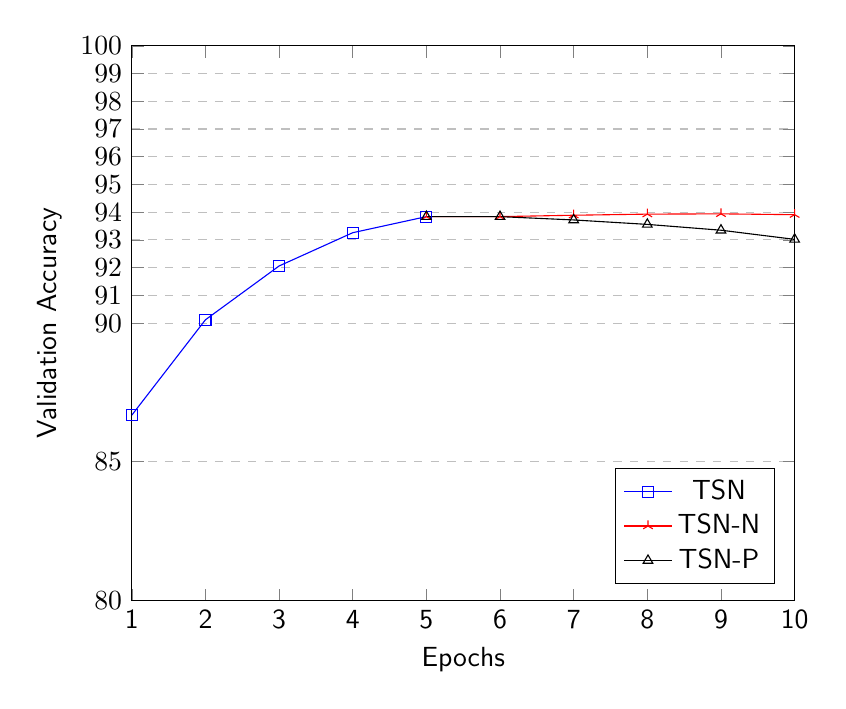
\begin{tikzpicture}
    \label{chart:fgsm}
    \begin{axis}[
        xlabel={Epochs},
        ylabel={Validation Accuracy},
        xmin=1, xmax=10,
        ymin=80, ymax=100,
        xtick={1,2,3,4,5,6,7,8,9,10},
        ytick={80,85,90,91,92,93,94,95,96,97,98,99,100},
        legend pos=south east,
        ymajorgrids=true,
        grid style=dashed,
        xticklabels={1,2,3,4,5,6,7,8,9,10}
    ]
    
    \addplot[
        color=blue,
        mark=square,
        ]
        coordinates {
        (1,86.68)(2,90.12)(3,92.06)(4,93.26)(5,93.84)
        };
        \addlegendentry{TSN}
        
    \addplot[
        color=red,
        mark=Mercedes star, % lewis hamilton bre
        ]
        coordinates {
        (5,93.84)(6,93.84)(7,93.89)(8,93.93)(9,93.94)(10,93.91)
        };
        \addlegendentry{TSN-N}
        
    \addplot[
        color=black,
        mark=triangle,
        ]
        coordinates {
        (5,93.84)(6,93.84)(7,93.72)(8,93.56)(9,93.35)(10,93.02)
        };
        \addlegendentry{TSN-P}
        
    \end{axis}
    \end{tikzpicture}
    \caption{Comparison of Siamese Model fine-tuning techniques. TSN network is unmodified Triplet loss Siamese Network, TSN-N is the same network with the positive side ignored for updates and the TSN-P is the same network with the negative side ignored for updates. TSN-N network manages to increase accuracy while the TSN-P network degrades it. Final (best) accuracies: 93.84\% (TSN), 92.92\% (TSN-P), 93.91\% (TSN-N)}
    \label{fig:snn_chart}
\end{figure}

Another idea is to use some combination of training similar to our method. For example we could try to train only with negative side first and then fine-tune with the positive or both sides. We could also use negative/positive side only if we detect that the learning process is stuck in some local minimum. We tried various combinations and can conclude that for initial training both sides of the network are necessary or the error becomes to large to minimize during training. In Figure \ref{fig:snn_chart} we demonstrate that negative fine-tuning outperforms positive fine-tuning when both sides of the Siamese model are used for pre-training.

\chapter{Negative Deep Reinforcement Learning}

In this part of the dissertation we discuss negative learning suitable for agent environments, namely with Deep Reinforcement Learning algorithms.

Reinforcement learning (RL) is a field in agent-based artificial intelligence. \cite{russell2002artificial} Main parts of defining a RL problem are the agent and the environment. The environment can be seen as "outside world" full of parameters and interactions in which the agent lives and interacts. At every stem the agent has a partial or complete observation of the state of the world and based on that state decides which action to take. The environment can also change based on the agent's decision.

Another important point is the concept of a reward signal. A reward is a signal from the environment which the agent receives and it denotes how "good" or "bad" the current world state is. The goal of the agent is to maximize its cumulative reward, sometimes called return. All RL algorithms model ways how the agent can learn to behave in order to maximize the return and achieve its goal.

When talking about RL algorithms, one important distinction is whether the environment has discrete action spaces or continuous actions spaces. In an environment with a discrete action space only a finite number of moves (actions) are available to the agent while in the continuous action space environments (e.g. robotic hands) we do not have a finite number of moves and the actions are real-valued vectors (e.g. move hand 10 centimeters over x axis). This distinction is important because it dictates our algorithm selection as some algorithms work better in discrete action spaces and some algorithms can only be applied to one type of the action space.

Another important term is policy. Policy (sometimes called simply agent) is a rule used by the agent to make decisions. In RL we use parametrized policies: policies whose outputs are computable functions that depend on a set of parameters (e.g. weights of a neural network) which we can adjust to modify behaviour. 


\section{Motivation and use-cases} 

% https://towardsdatascience.com/applications-of-reinforcement-learning-in-real-world-1a94955bcd12

Agent environment artificial intelligence has found many uses over the years. From game programming to path finding navigation software a problem formulation of agent and a changeable environment has been a foundation of computer science. In this section we mention some of recent use cases to demonstrate the importance and possibilities of Deep RL algorithms.

First interesting use case is described in "Resource Management with Deep Reinforcement Learning" \cite{mao2016resource} where it is shown how a RL model can be trained to automatically schedule computing resources and jobs with the objective to minimize waiting time thus optimizing throughput of extremely large computer systems.

Another use case where RL represents a state-of-the-art solution is in the Traffic Light Control problem \cite{wiering2000multi}, where a RL algorithm can be designed to control traffic lights. The model takes into count traffic flow in lanes and current light states to predict and generally optimize the traffic flow.

Of course, usage of reinforcement learning algorithms has found great success in real-world agent problems -- robotics. Some novel approaches even include models which can learn from raw videos of humans (or robots) doing different tasks and replicating that behaviour. \cite{mnih2015human}

Lastly we mention games, where RL algorithms dominate model leaderboards in different competitions. \cite{mnih2013playing} \cite{silver2016mastering} Game agent development was the use case which really showed the possibilities in using these models. It is not rare that these algorithms achieve super-human performance on various games beating even most skillful of players. The most famous algorithms surely is Google's AlphaGo an algorithm which can play the game of Go, a very complex board game.

\section{Deep Q Learning}

% https://towardsdatascience.com/deep-q-learning-tutorial-mindqn-2a4c855abffc

% https://www.tensorflow.org/agents/tutorials/0_intro_rl

Deep Reinforcement Learning is a relatively new and exciting field of Machine Learning which aims to use new and modern Deep Learning models as agents for Reinforcement Learning problems.

In (Deep) Reinforcement Learning we split the models into two large groups: model-free and model-based RL algorithms. Model-free RL algorithms learn a direct mapping of state to action. Policy gradient methods are one example of a model-free algorithm. Model-based algorithms work differently in that they learn a model of their environment as an intermediate step in learning. Then the agent's reward and return needs to be maximized. Q-Learning is a model-based algorithms because in the process of learning a Q-Table is created and this table maps states to actions.

A Q-table in non-deep Q-Learning is an actual table of state-action, q-value pairs. At the beginning of training it is initialized to all zero values. The table is used as "memory" to keep states, actions and their expected rewards. Q-value represents the estimated optimal (maximum) future value of the reward. The agent will randomly try actions and memorize what reward they have brought. In this trial and error process the environment is modeled and remembered for future attempts where the best known action is chosen.

There have been various upgrades to the Q-Learning algorithm. One particularly interesting is the Epsilon-Greedy Exploration Strategy in which the agent sometimes (randomly) chooses a random action instead of the known optimal one. This is so the agent gains more experience and possibly finds better actions for states for future use.

Updates to the Q-Table are done by using the Bellman Equation \cite{baird1999gradient} (Equation \ref{eq:Bellman}).

\begin{equation}
\label{eq:Bellman}
Q(S_t, A_t) = (1 - \alpha) Q(S_t, A_t) + \alpha * (R_t + \lambda * max_a Q(S_t+1, a))
\end{equation}

In the Bellman's equation, S represents the state, A represents the action, R represents the reward from taking A, t is the time stamp, \(\alpha\) is learning rate and the \(\lambda\) is the discount factor. The \(\lambda\) discount factor causes rewards to lose their value over time so more approachable immediate rewards are valued more highly. This is a regularization technique which prevents local optimums.

In Deep Q-Learning the Q-Table is replaced with a neural network (DQN \cite{mnih2013playing}). The neural network model learns patterns in states so it can map input states to (action, Q-value) pairs. Deep Q-Learning models usually suffer from instability in large action spaces, and this is the reason most implementations have two networks (main, target) with the same architecture but different weights. The goal of this is to allow our algorithm to backtrack in learning by replacing the weights between the two networks periodically. The architecture of the DQN is very simple. The input nodes are containing values that embed the state. The output nodes represent the actions. Every output node represents a certain action while the value of the node is the action's q-value. 

The weight updates are a bit different than traditional neural network models as a concept called Experience Replay is used. The main network samples and trains on a batch of past experiences which are gathered for a number of steps. The main network weights are then copied to the target network after a number of batches.

Experience Replay (ER) is a concept in RL and it can be summarised as storing and replaying environment states (\emph{state, action, reward, next-state}). The algorithm then learns from this data. Experience Replay can be used in off-policy algorithms to learn in offline fashion. Deep Q-Learning uses ER to learn in batches in order to prevent the model from "wandering" away in a series of wrong actions.

\section{Negative Rewards and Punishments}

In terms of negative learning and reinforcement learning, a formulation where negative learning is used in agent environments is very natural. As we mentioned a key component of learning in RL algorithms is the connection between state space, action space and most importantly here the reward function. Reward function controls the agent behaviour because we are always optimizing the behaviour so that the reward is maximized. Therefore, to define a negative learning in agent environments we simply define a reward function which only gives insight to the agent of which actions are the worst. There could be many actions with neutral or positive reward value but we do not optimize for that subset of actions. We only teach the agent what not to do or in other words what action not to choose in any situation. We define negative actions as actions which the agent "should not take".

\subsection{Collision Avoidance in Open Environments with Negative Deep Reinforcement Learning}

One example where this type of agent is beneficial can be easily described with collision avoidance systems. In a collision avoidance system it usually is not important which action is chosen by the agent if the action that is chosen is not leading to failure (collision). A cumulative reward of 0 is perfect as this means there is no penalties for collisions. One real-world example would be in self-driving cars or birds in the sky. If we imagine that the sky is an infinite space in which several agents are operating (flying) we can define a well rewarded system by defining a system in which the agents do not collide and continue operating. This system can be defined only by defining negative rewards (punishments) where a collision is to be avoided. Positive and neutral rewards are implicit and not defined in this system. For experimentation, this environment has been defined as a OpenAI gym environment. OpenAI Gym is a collection of environments for agent training and testing as well a set of interfaces for defining new environments. This environment's goal is to show a proof of concept results that training negative agents (agents with only negative rewards) is possible. In the current implementation we only experimented with negative rewards, but it is also possible to experiment with negative actions. In this environment we have four possible actions: move up, down, left and right. Negative action can be defined as "do not move right" for example. In this case the agent would randomly choose any of the three remaining actions. We experimented with this approach and while it is possible to implement it is inherently more unstable than just using normal actions. It is possible that for some environments negative actions are necessary and that is why we mention them here.

\subsection{Implementation}

For testing a full DQN simulation environment was created (Figure \ref{fig:bird}). In the environment we have the main agent (bird) and the obstacles. The obstacles move at constant speed in randomly selected direction and change direction upon colliding with edges of the environment, while the agent is either human or machine controlled. The number of obstacles and the velocity of obstacles is fully configurable. The agent has four possible actions which are moving itself by small amount to either of the four directions: up, down, left right. Action space is a vector of size 4 where only one element has a positive value (one hot vector). State is described as a vector of size \( size = 2 + 4 * O \) where \( O \) is the number of obstacles. The \( 2 \) values are the \( x \) and \( y \) coordinates of the agent and we add four additional values (\( x \) and \( y \) coordinates, and \( dx \) and \( dy \) movement vector) for every obstacle. We add the movement vector of the obstacles so the agent can predict the movement of them and react accordingly.

\begin{figure}[!ht]
  \centering
  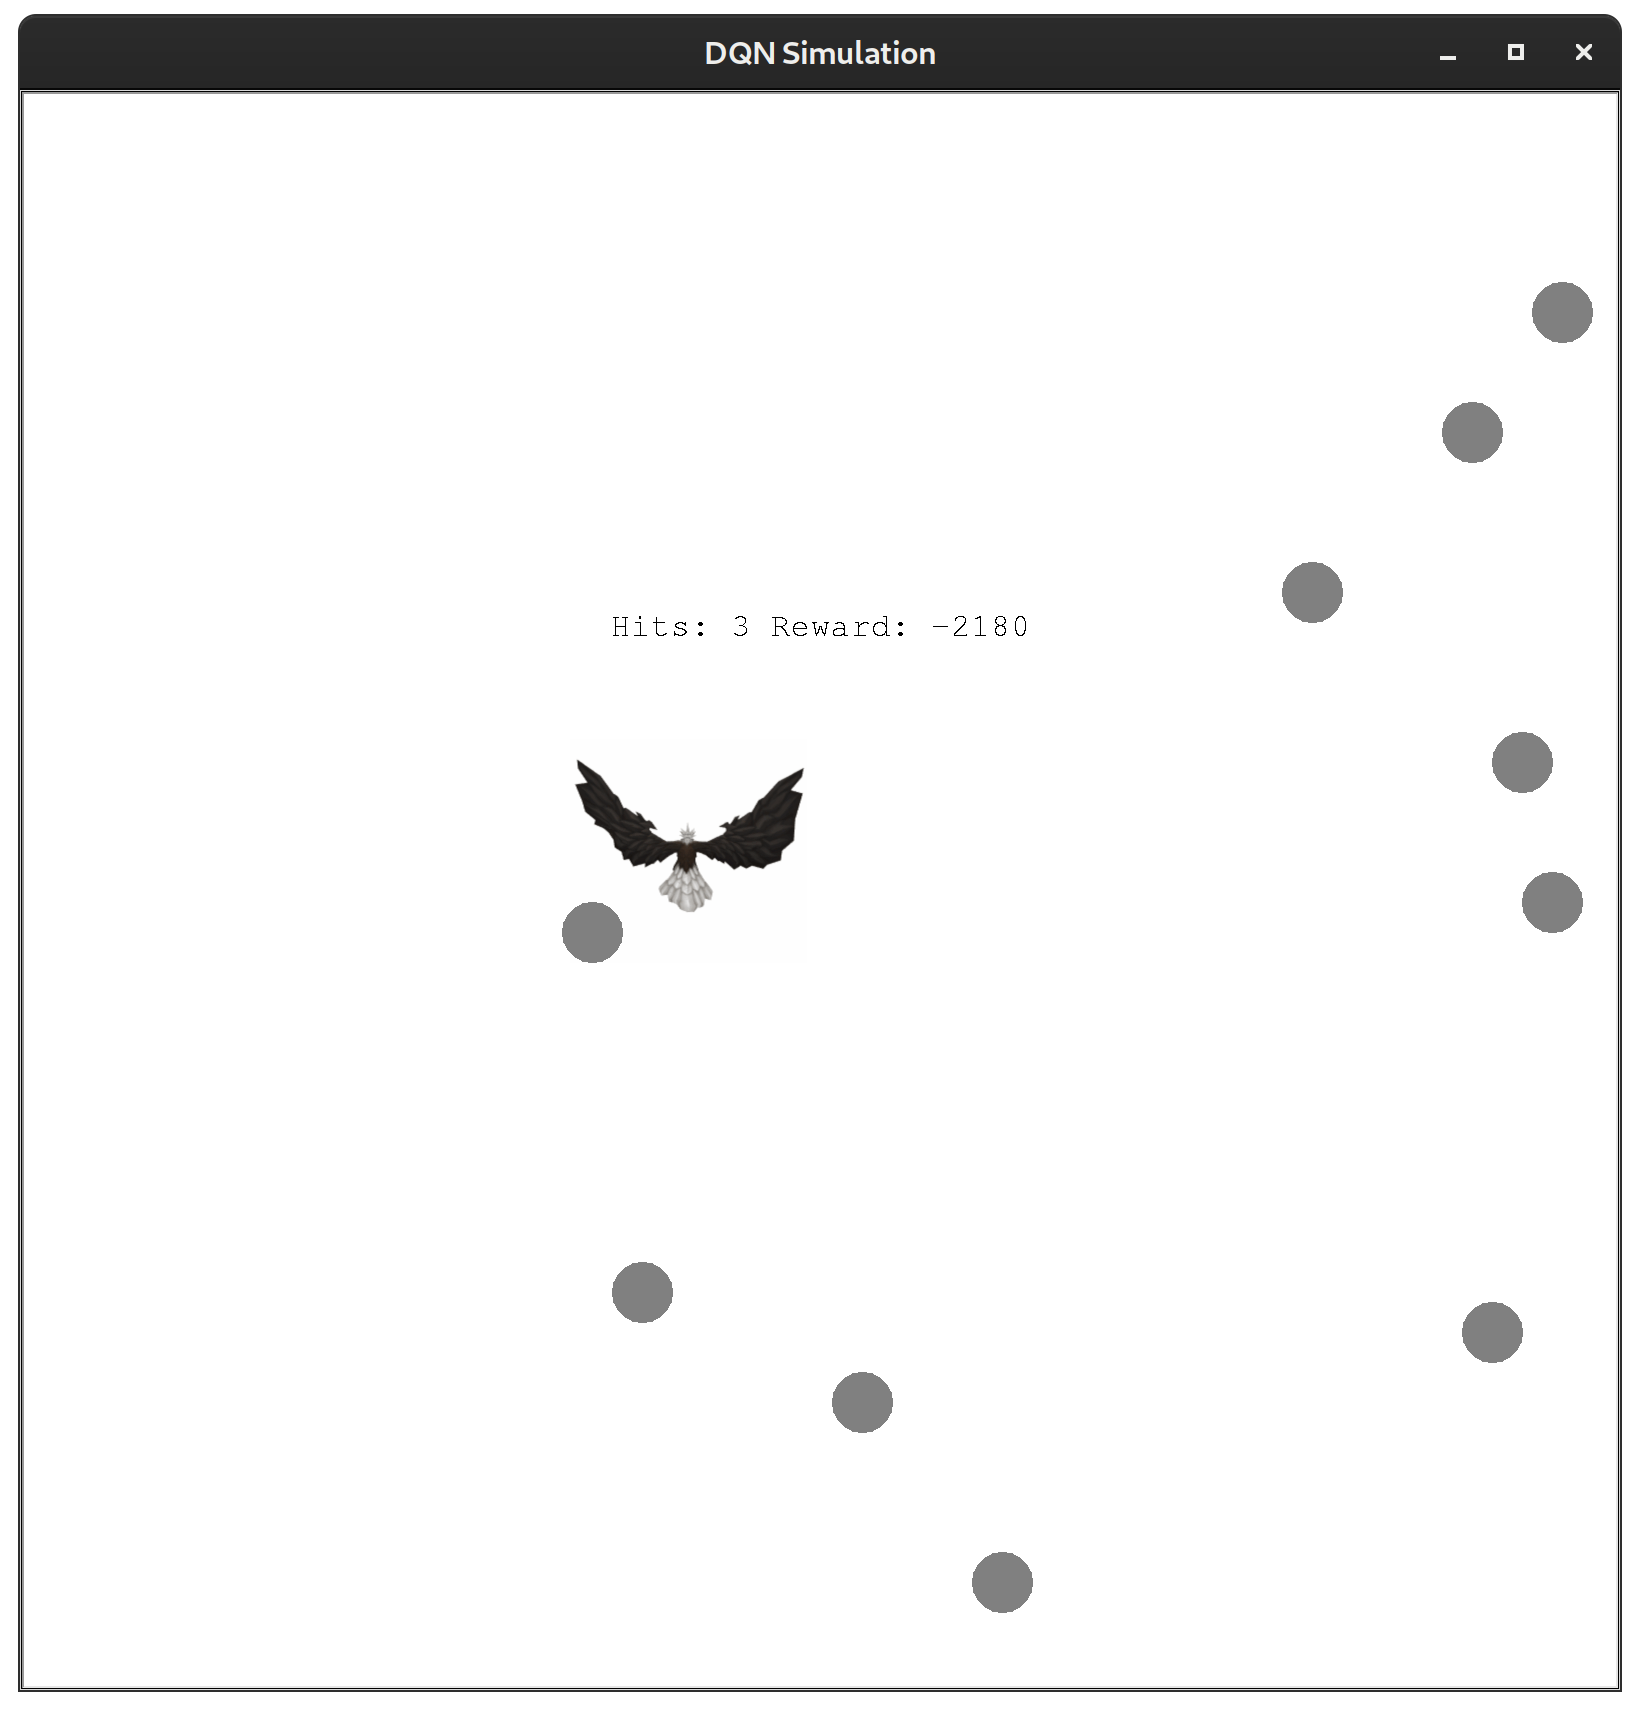
\includegraphics[scale=0.1]{figures/dqn_bird.png} 
  \caption{Example DQN environment for testing using only negative rewards (punishments). A bird is the agent and the grey dots are the obstacles that need to be avoided. Implementation with turtle Python module and Keras (TensorFlow).}
  \label{fig:bird}
\end{figure}

\subsubsection{Model performance and results}

For solving this environment a standard DQN algorithm implementation was used. 

The main point of the implementation is that the policy is implemented in a completely negative way. Agent is only told what actions it must not take to solve the solution. Agent is penalized for collisions and movements (to avoid unnecessary movements) and is never rewarded in any way. A cumulative reward of 0 is the perfect outcome for the agent and the closer the reward is to 0 the agent performs better. In the experiment (result shown in \ref{fig:birdr}) the model converges quickly even without positive rewards and tends to have the cumulative reward around zero for most episodes. It usually never manages the perfect score of zero (no movement, no collisions) as small movemements are necessary to avoid obstacles. The model has been tested with varying number of obstacles (up to 500) and different parameters (starting positions, obstacle movement vectors etc.). To account for stochasticity of the model, several runs were made, all with very similar results and convergence times.  

\begin{figure}[!ht]
  \centering
  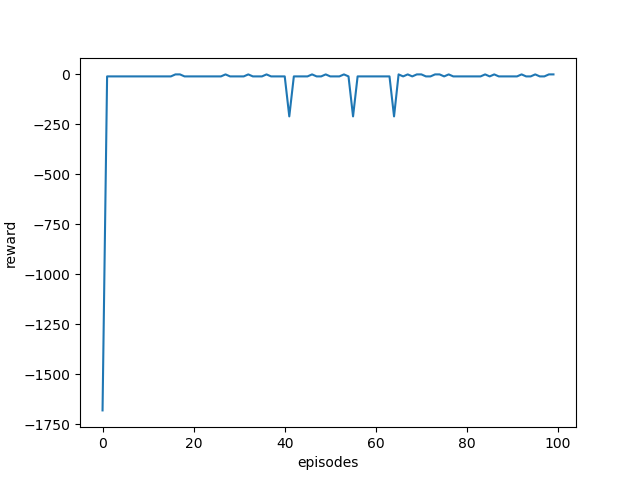
\includegraphics[scale=0.65]{figures/dqn_results.png} 
  \caption{DQN rewards for the open collision environment. Model converges quickly in just a few episodes bringing the reward to zero. Sudden "dips" in the reward plot represent model instability because the environment is stochastic i.e. the obstacles have randomized positions and movement vectors.}
  \label{fig:birdr}
\end{figure}

We believe this example is a good introductory step towards negative agent (policy) reinforcement learning models which can be used in conjunction with normal models or as standalone models. 

\chapter{Thesis Conclusions and Future Work}

This section provides a brief overview of the conclusions and planned future work. Some of the conclusions and future work plans have also been included in specific parts of the thesis and omitted here.

To conclude, in this PhD thesis we defined and experimented with Negative Deep Learning models. We introduce several models that exist today and propose and implement new ones. We also show various ways of creating negative models and we believe a very important paradigm: combination of positive (normal) and negative models and positive and negative training.

For the CBOMF model and Synergy model we show that these models have increased robustness and performance (sometimes more than 10\% accuracy increase) in difficult scenarios such as occlusions or adversarial examples, both white-box and black-box.

We experiment in great depth with feature negation process, testing different activation functions, negative convolutions and other modifications of the process we defined in our previous works. We also mention some new ideas for negative learning models. Combination of positive and negative learning can be very useful in various scenarios as well as carefully selecting the ratio of positive and negative training data samples. We also experiment with different order of training for positive and negative learning, showing how to fine-tune existing normal models with negative learning techniques.

For the "true" negative deep learning models we introduce negative Siamese networks and show that they can be used for regularization and additional training of the models. We also show that negative learning has its place in agent environments and provide an example of negative policy algorithm in the form of Negative Deep Q-Learning algorithm and one of its possible use cases (obstacle avoidance system). We also discuss other possible true negative deep learning models and demonstrate what are the current issues with developing them further. For example, lack of negatively labeled dataset is the most apparent issue which we plan to solve with manual labeling of some widely known datasets in the future. Existing solutions, such as Negative Sampling as shown in Sections \ref{negsampling} and \ref{noisylabels} are flawed since they use stochasticity for creating negative samples from existing positive samples. The question is whether it is viable to do so, if we already have positive samples and know what is their label. This is why we also mention partial input training and partial input negative training as means to improve existing models.

Apart from the works presented in this thesis there is still a lot to experiment with. 

Firstly, we would like to experiment with other large network architectures which yield even greater results e.g. EfficientNet \cite{tan2019efficientnet} or DenseNet \cite{huang2017densely}. There, it would be interesting to see if our approach can push further state-of-the-art models.

Next, in this thesis we focused on classification problems while only providing ideas for future negative regression task implementation. It would be interesting to see how our approaches can be applied to regression tasks. One idea that we have already is to use our negative feature approach in multivariate time-series modelling where in some use cases a missing feature can be of very high importance for the resulting output.

The most promising aspect of this thesis would have to be the robustness to adversarial attacks. We first presented our findings here in this thesis and the results are very promising for both our negative feature approach and for the Synergy models. We will definitely generalize the experiments we performed here and continue working in this direction, which was also the initial direction we hoped our models would go.

For the negative agent models, we would like to continue working in a more complex or real environment. One that we hope to try out in the future is the CARLA \cite{dosovitskiy2017carla} environment, the most complete and complex self-driving environment where we would like to add our negative rules to the policy and define what the agent (self driving car) should never do.

Lastly, in this thesis we demonstrated that one of our approaches can be used as regularization step in training of Siamese models. We were not able to make the model to train completely in a negative-learning way which is something we think is possible. In the future we will definitely revisit this problem and try to see what the issue with the model was.

We would also like to experiment with several of the negative learning process uses presented in this thesis. For example, using negative learning to help overcome local minimums during training remains to be tested as well as various ordering of positive/negative training combinations and the ration of positive and negative training samples.

\part{Appendices}
\chapter{Source code and Reproducibility}
\label{source}

The source code for our models and the training processes can be found on the following link: 

\begin{footnotesize}
\url{github.com/nmilosev/phd}
\end{footnotesize}

We have taken some additional steps with the used libraries and tools so that our results are reproducible and testable in many different environments.

\backmatter

% there is no index, so it's disabled
% \printindex

% \skica{} use raggedright, had problems with urls and dois not breaking proper
% maybe there are better solutions
{
  \raggedright
  \printbibliography[heading=bibintoc]
}

% --------------------------------

\chapter{Prošireni izvod}



% --------------------------------

\chapter{Short Biography}


Nemanja Milošević was born on 20.11.1992 in Ruma.

He finished ``Jovan Jovanović Zmaj'' elementary school in Ruma in 2007,
followed by high school ``Gimnazija Stevan Puzić'', Ruma, in 2011. The same year he enrolled into the Faculty of Sciences in Novi Sad to study computer science. He obtained his BSc diploma in June of 2014, and a masters degree in September of 2016. In 2020 he participated in Erasmus+ Doctoral Student Exchange Program, studying at University of Coimbra, Portugal for six months.

He has been involved in teaching at the Department of Mathematics and
Informatics, Faculty of Sciences in Novi Sad, as a teaching and research assistant since 2016.

He has conducted theoretical and practical exercises in several
computer science courses for undergraduate and master students,
including Artificial Intelligence 1, Databases 1 and 2, Business Software Development, Python Development and Computer Networks.

He coauthored four papers as conference proceedings and
journal articles. He was a conference presenter more than ten times both on national and international conferences. He participated as a Machine Learning researcher on both national (GRASP - Graphs in Space: Graph Embeddings for Machine Learning on Complex Data) and international projects including H2020 projects (I-BiDaas - Industrial-Driven Big Data as a Self-Service Solution, C4IIOT - Cyber security 4.0: Protecting the Industrial Internet of Things).

He is an supporter of Open Source Software and a contributor to several open source software projects most notably, Fedora Project and PyTorch.

\vfill


\begin{tabbing}
  \hspace{0.7\textwidth} \= nebitan tekst \kill
  Novi Sad, 2021 \> Nemanja Milošević
\end{tabbing}

\begin{otherlanguage}{english}
\chapter{Kratka biografija}

Nemanja Milošević se rodio 20. novembra 1992. godine u Rumi.

Završio je osnovnu školu ``Jovan Jovanović Zmaj'' u Rumi 2007. godine, a zatim srednju školu ``Gimnazija Stevan Puzić`` u Rumi 2011. godine. Iste godine upisuje osnovne akademske studije informatike na Prirodno-matematičkom fakultetu u Novom Sadu. Završava trogodišnji program u junu 2014. godine a master diplomu dobija u septembru 2016. godine. 2020. godine učestvuje na Erasmus+ razmeni doktorskih studenata sa Univerzitetom u Koimbri, Portugal gde je bio doktorski student u šestomesečnom periodu.

Nemanja je asistent u nastavi na Departmanu za matematiku i informatiku Prirodno-matematičkog fakulteta u Novom Sadu od 2016. godine. Držao je vežbe iz nekoliko predmeta na osnovim i master studijama: Veštačka Inteligencija 1, Baze podataka 1 i 2, Razvoj poslovnih sistema, Računarske Mreže i Seminarski rad A - Python.

Nemanja je koautor na četiri rada objavljenim na međunarodnim konferencijama i u međunarodnim časopisima. Držao je više od deset predavanja na međunarodnim konferencijama. Kao istraživač u oblasti mašinskog učenja učestvovao je na državnim (GRASP - Graphs in Space: Graph Embeddings for Machine Learning on Complex Data) kao i na međunarodnim projektima uključujući i Horizon 2020 projekte I-BiDaaS i C4IIOT.

Otvoreno podržava razvoj slobodnog softvera i deo je razvojnog tima više projekata otvorenog koda od kojih su najznačajniji Fedora Project i PyTorch.

\vfill


\begin{tabbing}
  \hspace{0.7\textwidth} \= nebitan tekst \kill
  Novi Sad, 2021. \> Nemanja Milošević\\
  \\
  \> \makebox[0.3\textwidth]{\dotfill}
\end{tabbing}

\end{otherlanguage}

\newcounter{allpages}
\setcounter{allpages}{\value{frontmatterpage}}

\newcounter{mainpages}
\setcounter{mainpages}{\totalpages}

% offset the last increase
\addtocounter{mainpages}{-1}

\addtocounter{allpages}{\value{mainpages}}

\chapter[Ključna dokumentacijska informacija]{\Large Univerzitet u Novom Sadu\\
          Prirodno-matematički fakultet\\
          Ključna dokumentacijska informacija}
 
\noindent
\begin{tabbing}
  \hspace*{.3\textwidth}                                           \= \hspace*{.7\textwidth}        \kill
  Redni broj:                                                      \>                               \\
  RBR                                                              \>                               \\
  Identifikacioni broj:                                            \>                               \\
  IBR                                                              \>                               \\
  Tip dokumentacije:                                               \> Monografska dokumentacija     \\
  TD                                                               \>                               \\
  Tip zapisa:                                                      \> Tekstualni štampani materijal \\
  TZ                                                               \>                               \\
  Vrsta rada:                                                      \> Doktorska disertacija         \\
  VR                                                               \>                               \\
  Autor:                                                           \> \autor                        \\
  AU                                                               \>                               \\
  Mentor:                                                          \> dr Miloš Racković              \\
  MN                                                               \>                               \\
                                                                   \>                               \\
  Naslov rada:                                                     \> 
    \begin{minipage}[t]{.65\textwidth}
    \naslovsr
  \end{minipage}                                                                                    \\
  NR                                                               \>                               \\
  Jezik publikacije:                                               \> engleski                      \\
  JP                                                               \>                               \\
  Jezik izvoda:                                                    \> srpski/engleski               \\
  JI                                                               \>                               \\
  Zemlja publikovanja:                                             \> Srbija                        \\
  ZP                                                               \>                               \\
  Uže geografsko područje:                                         \> Vojvodina                     \\
  UGP                                                              \>                               \\
  Godina:                                                          \> 2021                          \\
  GO                                                               \>                               \\
                                                                   \>                               \\
  Izdavač:                                                         \> autorski reprint              \\
  IZ                                                               \>                               \\
  Mesto i adresa:                                                  \> Novi Sad, Trg D. Obradovića 4 \\
  MA                                                               \>                               \\
                                                                   \>                               \\
  Fizički opis rada:                                               \> \arabic{numchapter}%
  /\arabic{allpages} (\roman{frontmatterpage} + \arabic{mainpages})%
  /\arabic{citenum}%
  /\totaltables%
  /\totalfigures%
  /0%
  /\arabic{chapter}                                                                                 \\
  \hspace*{2\parindent}
  (broj poglavlja/strana/lit. citata/tabela/slika/grafika/priloga) \>                               \\
  FO                                                               \>                               \\
  Naučna oblast:                                                   \> Računarske nauke              \\
  NO                                                               \>                               \\
  Naučna disciplina:                                               \> Mašinsko učenje
            \\
  ND                                                               \>                               \\
  Predmetna odrednica                                              \>                               \\
  PO                                                               \>                               \\
  Ključne reči:                                                   \> 
    \begin{minipage}[t]{.65\textwidth}
      Veštačka inteligencija, Mašinsko učenje, Duboko učenje,
      Neuronske mreže, Konvolutivne neuronske mreže, Robustnost,
      Robustnost neuronskih mreža, Negativno učenje
    \end{minipage}                                                                                  \\
  UDK                                                              \>                               \\
  Čuva se:                                                         \>                               \\
  ČU                                                               \>                               \\
  Važna napomena:                                                  \>                               \\
  VN                                                               \>                               \\
  Izvod:                   \`
  \begin{minipage}[t]{.8\textwidth}
  U današnje vreme upotreba dubokog učenja radi prepoznavanja određenih paterna u podacima postala je nezamenljiv alat u mnogim sistemima. U kritičnim sistemima pogotovo, duboke neuronske mreže se često koriste čak i u scenarijima koji direktno utiču na naše živote. Upravo to je razlog što se u poslednje vreme u istraživanju sve više stavlja akcenat na duboko razumevanje ovih modela i na modele koji su dokazano pouzdani, robusni i sigurni za upotrebu.

U ovoj doktorskoj disertaciji istražujemo negativne modele dubokog mašinskog učenja kao novi pristup razvoju modela sa visokim performansama i još važnije sa povećanom robustnošću i pouzdanošću u poređenju sa modelima današnjice. Takođe se bavimo nadogradnjama postojećih modela sa našim negativnim pristupom i pokazujemo kako se postojeći modeli mogu unaprediti bez velikih promena u arhitekturi.

Kod modela za klasifikaciju slika (danas najrasprostranjenija primena dubokih konvolutivnih neuronskih mreža) pokazaćemo kako se ovi modeli mogu nadograditi i izmeniti kako bi u obzir uzimali i negativne osobine -- one osobine koje znamo da postoje a nisu trenutno prisutne u ulaznim podacima.

Za sve modele predstavljene u ovoj disertaciji biće prikazana duboka analiza procesa kao što su negacije osobina, negativne aktivacione funkcije, zamrzavanje slojeva neuronskih mreža, transfer znanja iz jedne mreže u drugu, fine-tuning pristup treniranju, inverzije konvolutivnih filtera i drugo.

\end{minipage}\\

\ \`
\begin{minipage}[t]{.8\textwidth}
  Dodatno znanje, u obliku negativnog znanja, može biti veoma bitan faktor u učenju i kreaciji modela koji imaju povećanu preciznost, pouzdanost i robustnost, pogotovo u teškim situacijama. Definišemo teške situacije kao one situacije u kojima je model suočen sa podacima koji su izmenjeni ili teži za razumevanje na neki način, bilo na prirodan način ili veštački način. Na primer, modeli predstavljeni u ovom radu su testirani u slučajevima parcijalnih ulaza i okluzija gde su delovi ulaznih podataka odstranjeni ili zaklonjeni na neki način. Negativni modeli u ovakvim situacijama imaju znatno više performanse u poređenju sa običnim, tradicionalnim modelima iste arhitekture. Za veštački generisane situacije, govorićemo o adversarijalnim mrežama, podacima i napadima i kakve su performanse naših negativnih modela kada se suoče sa takvim podacima. Testirani su black-box i white-box adversarijalni napadi i odabrani su oni napadi koji danas predstavljaju najnaprednije moguće metode za namerna kvarenja modela dubokog učenja.

U ovoj disertaciji takođe uvodimo pojam mreže sinergije, koja predstavlja spoj normalne i negativne mreže i kao takva se može koristiti i primeniti na bilo koji postojeći model. U sinergiji deo mreže ili cela mreža se dodaje na postojeći model u kombinaciji sa određenim modifikacijama kako bi se uključilo negativno duboko učenje. Pokazaćemo da ovakvi modeli imaju još više performanse u poređenju sa negativnim modelima i eksperimentisaćemo sa raznim načinima spajanja mreža. Model sinergije će biti testiran na CIFAR10 skupu podataka dok su negativni modeli razvijani i testirani na MNIST i EMNIST skupovima podataka.

Na kraju, govorićemo o modelima koji koriste "pravo" negativno učenje, a to su oni modeli koji koriste samo negativno znanje za učenje. Biće dat prikaz postojećih sličnih modela kao što su Negative Sampling modeli, Noisy Label Classification modeli i modeli koji koriste Noise Contrastive Estimation. Naš fokus je na dva modela za koje ćemo predložiti i implementirati nadogradnje a to su: negativna Deep Q-Learning agentska neuronska mreža i negativna sijamska Triplet Loss mreža. Oba ova modela mogu biti korišćena uz pomoć samo negativnih podataka, u nekim slučajevima za potpuno treniranje a u nekim slučajevima kao vid regularizacije.
    \end{minipage}                                          \\
  IZ                       \>                               \\
  Datum prihvatanja teme od strane \>                       \\
  Senata:                 \> 25.06.2020.                     \\
  DP                       \>                               \\
  Datum odbrane:           \>                     \\
  DO                       \>                               \\
  Članovi komisije:        \>                               \\
  \hspace*{\parindent}
  (Naučni stepen/ime i prezime/zvanje/fakultet) \>          \\
  KO                       \>                               \\
  Predsednik:              \`
    \begin{minipage}[t]{.7\textwidth}
    dr Srđan Škrbić, redovni profesor,\\
    Univerzitet u Novom Sadu, Prirodno-matematički fakultet
    \end{minipage}                                          \\
  Mentor:                    \`
    \begin{minipage}[t]{.7\textwidth}
    dr Miloš Racković, redovni profesor,\\
    Univerzitet u Novom Sadu, Pri\-ro\-d\-no-ma\-te\-ma\-ti\-č\-ki fakultet
    \end{minipage}                                          \\
  Član:                    \`
    \begin{minipage}[t]{.7\textwidth}
    dr Miloš Radovanović, profesor,\\
    Univerzitet u Novom Sadu, Prirodno-matematički fakultet
    \end{minipage}                                          \\
  Član:                    \`
    \begin{minipage}[t]{.7\textwidth}
    dr Jelena Slivka, docent,\\
    Univerzitet u Beogradu, Fakultet tehničkih nauka
    \end{minipage}                                          \\
  Član:                    \`
    \begin{minipage}[t]{.7\textwidth}
    dr Vladimir Lončar, naučni saradnik,\\
    Institut za fiziku, Zemun
    \end{minipage}                                          \\
\end{tabbing}
%%%%%%%%%%%%%%%%%%%%%%%%%%%%%%%%%%%%%%%%%%%%%%%%%%%%%%%%%%%%%%%%%% 5%%%%%%%%%%%%%

\chapter[Key Words Documentation]{\Large University of Novi Sad\\
          Faculty of Science\\
          Key Words Documentation}
 
\noindent
\begin{tabbing}
  \hspace*{.3\textwidth}   \= \hspace*{.7\textwidth}        \kill
  Accession number:        \>                               \\
  NO                       \>                               \\
  Identification number:   \>                               \\
  INO                      \>                               \\
  Document type:           \> Monograph documentation       \\
  DT                       \>                               \\
  Type of record:          \> Textual printed material      \\
  TR                       \>                               \\
  Contents code:           \> Doctoral dissertation             \\
  CC                       \>                               \\
  Author:                  \> \autor                  \\
  AU                       \>                               \\
  Mentor:                  \> Dr.~Miloš Racković          \\
  MN                       \>                               \\
                           \>                               \\
  Title:                   \>
    \begin{minipage}[t]{.7\textwidth}
      \naslov
    \end{minipage}                                          \\
    TI                       \>                               \\
    Language of text:        \> English                       \\
    LT                       \>                               \\
    Language of abstract     \> Serbian/English               \\
    LA                       \>                               \\
    Country of publication:  \> Serbia                        \\
    CP                       \>                               \\
    Locality of publication: \> Vojvodina                     \\
    LP                       \>                               \\
    Publication year:        \> 2021                          \\
    PY                       \>                               \\
    \>                               \\
    Publisher:               \> Author's reprint              \\
    PU                       \>                               \\
    Publ. place:             \> Novi Sad, Trg D.~Obradovića 4 \\
    PP                       \>                               \\
    \>                               \\
    Physical description:    \> \arabic{numchapter}%
/\arabic{allpages} (\roman{frontmatterpage} + \arabic{mainpages})%
/\arabic{citenum}%
/\totaltables%
/\totalfigures%
/0%
/\arabic{chapter}\\
    \hspace*{\parindent}
    (no. chapters/pages/bib.~refs/tables/figures/graphs/appendices)\> \\
    PO                       \>                               \\
    Scientific field:        \> Computer Science              \\
    SF                       \>                               \\
    Scientific discipline:   \> Machine Learning  \\
    SD                       \>                               \\
    Subject/Key words: \>
    \begin{minipage}[t]{.65\textwidth}
      Artificial Intelligence, Machine Learning, Deep Learning,
      Neural Networks, Convolutional Neural Networks, Robustness,
      Neural Network Robustness. Negative Learning
    \end{minipage}                                          \\
  SKW                      \>                               \\
  UC                       \>                               \\
  Holding data:            \>                               \\
  HD                       \>                               \\
  Note:                    \>                               \\
  N                        \>                               \\
  Abstract:                \`
  \begin{minipage}[t]{.8\textwidth}
    In recent times the use of Deep Learning as a tool for pattern recognition and more has become essential for many tasks. In critical systems specifically these models are often used in human life affecting environments and that is the reason for new and recent research regarding these models and and their robustness and reliability. 

In this thesis we explore negative deep learning as a new approach to developing models which have higher performance and more importantly increased robustness compared to normal models used today. Moreover we show how many existing models can be upgraded to employ some kind of negative deep learning without large architectural changes.

We will discuss how image classification neural networks (most popular use case of the convolutional neural network family) can be modified to take into consideration missing (negative) features from input samples when making their decisions. 

We provide deep explanation of the feature negating process, experimenting with different activation functions, neural network layer freezing, Transfer Learning and Fine Tuning approaches, convolutional kernel inversions and more.
\end{minipage}\\
\  \`
\begin{minipage}[t]{.8\textwidth}
  We show that by employing this additional knowledge we create models with increased robustness, especially in difficult scenarios. We define difficult scenarios as those which are naturally or artificially difficult for modern neural networks. For example, we benchmark our models in the cases of partial input examples and occlusion against normal models of same architecture to show our modifications bring performance and robustness is this type of classification tasks. For artificial scenarios, we show that our models are less susceptible to adversarial attacks, both white-box and black-box. We test with state-of-the-art adversarial algorithms and see various level of improvements for different attacks and datasets (MNIST, EMNIST variants).

In this thesis we also introduce the notion of a Synergy model, a model which is a pure upgrade of any neural network model where additional model, or part of it, is appended with the negativity embedded into the underlying signal processing. We show that the Synergy models can generally outperform our negative models without any performance penalty when comparing to normal models. We also experiment with different state-of-the-art Ensemble network joining methods and show how they differ in implementation effort and performance. The synergy models is tested against more complex CIFAR10 dataset and its adversarial modifications, both human and artificial.

Lastly we mention true negative deep learning models, which are those which use only negative knowledge for learning. An overview of existing models is provided including Negative Sampling, Noisy Label Classification and Noise Contrastive Estimation. We focus on two models for which we provide upgrades and implementations: a negative Deep Q-Learning agent in a Deep Reinforcement Learning Task and a negative-only Siamese Triplet Loss network. Both these models, we show, can be used in a negative-only scenarios, some for regularization purposes, some for complete training.
    \end{minipage}                                          \\
  AB                       \>                               \\
  Accepted on Senate: \>   25.06.2020.      \\
  AS                       \>                               \\
  Defended:                \>                        \\
  DE                       \>                               \\
  \begin{minipage}[t]{.7\textwidth}
    Thesis Defend Board:\\
    \hspace*{\parindent}(Degree/first and last name/title/faculty)
  \end{minipage}\>             \\
  DB                       \>                               \\
  President: \`
    \begin{minipage}[t]{.7\textwidth}
    Dr.~Srđan Škrbić, full professor,\\
    University of Novi Sad, Faculty of Sciences
    \vspace*{1mm}
    \end{minipage}                                          \\
  Mentor:                  \`
    \begin{minipage}[t]{.7\textwidth}
    Dr.~Miloš Racković, full professor,\\
    University of Novi Sad, Faculty of Sciences
    \vspace*{1mm}
    \end{minipage}                                          \\
  Member:                  \`
    \begin{minipage}[t]{.7\textwidth}
    Dr.~Miloš Radovanović, professor,\\
    University of Novi Sad, Faculty of Sciences
    \vspace*{1mm}
    \end{minipage}                                          \\
  Member:                  \`
    \begin{minipage}[t]{.7\textwidth}
    Dr.~Jelena Slivka, assistant professor,\\
    University of Novi Sad, Faculty of Technical Sciences
    \vspace*{1mm}
    \end{minipage}                                          \\
  Member:                  \`
    \begin{minipage}[t]{.7\textwidth}
    Dr.~Vladimir Lončar, research associate,\\
    Institute of Physics, Zemun
    \vspace*{1mm}
    \end{minipage}                                          \\
\end{tabbing}

\end{document}
